
\section{Additional Simulation Parameters}
\label{section:add}

\subsection{Constraints and Restraints}
\label{section:config_add}

\subsubsection{Harmonic constraint parameters}

The following describes the parameters for the 
harmonic constraints feature of \NAMD.  Actually, this feature 
should be referred to as harmonic restraints rather than 
constraints, but for historical reasons the terminology of 
harmonic constraints has been carried over from X-PLOR.  
This feature allows a harmonic restraining force to be applied 
to any set of atoms in the simulation.

\begin{itemize}

\item
\NAMDCONFWDEF{constraints}{are constraints active?}{{\tt on} or {\tt off}}{{\tt off}}
{Specifies whether or not harmonic constraints are active.  If it 
is set to {\tt off}, then no harmonic constraints are computed.  
If it is set to {\tt on}, then 
harmonic constraints are calculated using the values specified 
by the parameters {\tt consref}, {\tt conskfile}, {\tt conskcol}, 
and {\tt consexp}.}

\item
\NAMDCONFWDEF{consexp}{exponent for harmonic constraint energy function}{positive, even integer}{2}
{Exponent to be use in the harmonic constraint energy function.  
This value must be a positive integer, and only even values really make 
sense.  This parameter is used only if {\tt constraints} is set to 
{\tt on}.}

\item
\NAMDCONF{consref}{PDB file containing constraint reference positions}{UNIX file name}
{PDB file to use for reference positions for harmonic constraints.  
Each atom that has an active constraint will be constrained about 
the position specified in this file.}

\item
\NAMDCONF{conskfile}{PDB file containing force constant values}{UNIX filename}
{PDB file to use for force constants for 
harmonic constraints.}

\item
\NAMDCONF{conskcol}{column of PDB file containing force constant}{{\tt X}, {\tt Y}, {\tt Z}, {\tt O}, or {\tt B}}
{Column of the PDB file to use for the harmonic constraint force constant.
This parameter may specify any of the floating point fields of the PDB file, 
either X, Y, Z, occupancy, or beta-coupling (temperature-coupling).  
Regardless of which column is used, a value of 0 indicates that the atom 
should not be constrained.  
Otherwise, the value specified is used as the force constant for 
that atom's restraining potential.}

\item
\NAMDCONFWDEF{constraintScaling}{scaling factor for harmonic constraint energy function}{positive}{1.0}
{The harmonic constraint energy function is multiplied by this parameter,
making it possible to gradually turn off constraints during equilibration.
This parameter is used only if {\tt constraints} is set to 
{\tt on}.}

\item
\NAMDCONFWDEF{selectConstraints}{Restrain only selected Cartesian components of the coordinates?}{{\tt on} or {\tt off}}{{\tt off}}
{This option is useful to restrain the positions of atoms to a plane or a line in space. If active,
 this option will ensure that only selected Cartesian components of the coordinates are restrained.
 E.g.: Restraining the positions of atoms to their current z values with no restraints
 in x and y will allow the atoms to move in the x-y plane while retaining their original z-coordinate.
 Restraining the x and y values will lead to free motion only along the z coordinate.}

\item
\NAMDCONFWDEF{selectConstrX}{Restrain X components of coordinates}{{\tt on} or {\tt off}}{{\tt off}}
{Restrain the Cartesian x components of the positions.}
\item
\NAMDCONFWDEF{selectConstrY}{Restrain Y components of coordinates}{{\tt on} or {\tt off}}{{\tt off}}
{Restrain the Cartesian y components of the positions.}
\item
\NAMDCONFWDEF{selectConstrZ}{Restrain Z components of coordinates}{{\tt on} or {\tt off}}{{\tt off}}
{Restrain the Cartesian z components of the positions.}

\end{itemize}

\subsubsection{Fixed atoms parameters}

Atoms may be held fixed during a simulation.  \NAMD\ avoids calculating most interactions in which all affected atoms are fixed unless {\tt fixedAtomsForces} is specified.

\begin{itemize}

\item
\NAMDCONFWDEF{fixedAtoms}{are there fixed atoms?}{{\tt on} or {\tt off}}{{\tt off}}
{Specifies whether or not fixed atoms are present.} 

\item
\NAMDCONFWDEF{fixedAtomsForces}{are forces between fixed atoms calculated?}{{\tt on} or {\tt off}}{{\tt off}}
{Specifies whether or not forces between fixed atoms are calculated.  This option is required to turn fixed atoms off in the middle of a simulation.
These forces will affect the pressure calculation, and you should leave this option off when using constant pressure if the coordinates of the fixed atoms have not been minimized.
The use of constant pressure with significant numbers of fixed atoms is not recommended.}

\item
\NAMDCONFWDEF{fixedAtomsFile}{PDB file containing fixed atom parameters}
{UNIX filename}{{\tt coordinates}}
{PDB file to use for the fixed atom flags for each atom.  
If this parameter is not specified, then 
the PDB file specified by {\tt coordinates} is used.}

\item
\NAMDCONFWDEF{fixedAtomsCol}{column of PDB containing fixed atom parameters}
{{\tt X}, {\tt Y}, {\tt Z}, {\tt O}, or {\tt B}}{{\tt O}} 
{Column of the PDB file to use for the containing fixed atom parameters for 
each atom.  The coefficients can be read from any 
floating point column of the PDB file.  
A value of 0 indicates that the atom is not fixed.}

\end{itemize}

\subsection{Energy Minimization}

\subsubsection{Conjugate gradient parameters}

The default minimizer uses a sophisticated conjugate gradient and
line search algorithm with much better performance than the older
velocity quenching method.
The method of conjugate gradients is used to select successive search
directions (starting with the initial gradient) which eliminate
repeated minimization along the same directions.
Along each direction, a minimum is first bracketed (rigorously bounded)
and then converged upon by either a golden section search, or, when
possible, a quadratically convergent method using gradient information.

For most systems, it just works.

\begin{itemize}

\item
\NAMDCONFWDEF{minimization}{Perform conjugate gradient energy minimization?}{{\tt on} or {\tt off}}{{\tt off}}
{Turns efficient energy minimization {\tt on} or {\tt off}.}

\item
\NAMDCONFWDEF{minTinyStep}{first initial step for line minimizer}{positive decimal}{1.0e-6}
{If your minimization is immediately unstable, make this smaller.}

\item
\NAMDCONFWDEF{minBabyStep}{max initial step for line minimizer}{positive decimal}{1.0e-2}
{If your minimization becomes unstable later, make this smaller.}

\item
\NAMDCONFWDEF{minLineGoal}{gradient reduction factor for line minimizer}{positive decimal}{1.0e-4}
{Varying this might improve conjugate gradient performance.}

\end{itemize}

\subsubsection{Velocity quenching parameters}

You can perform energy minimization using a simple quenching
scheme.   While this algorithm is not the most rapidly convergent, it
is sufficient for most applications.  There are only two parameters
for minimization:  one to activate minimization and another
to specify the maximum movement of any atom.  

\begin{itemize}

\item
\NAMDCONFWDEF{velocityQuenching}{Perform old-style energy minimization?}{{\tt on} or {\tt off}}{{\tt off}}
{Turns slow energy minimization {\tt on} or {\tt off}.}

\item
\NAMDCONFWDEF{maximumMove}{maximum distance an atom can move during each step (\AA)}
{positive decimal}
{$0.75\times\mbox{{\tt cutoff}}/\mbox{{\tt stepsPerCycle}}$}
{Maximum distance that an atom can move during any single timestep of
minimization.  This is to insure that atoms do not go flying off into
space during the first few timesteps when the largest energy conflicts
are resolved.}

\end{itemize}

\subsection{Temperature Control and Equilibration}

\subsubsection{Langevin dynamics parameters}

\NAMD\ is capable
of performing Langevin dynamics, where additional damping and
random forces are introduced to the system.  This capability
is based on that implemented in X-PLOR which is detailed
in the X-PLOR {\it User's Manual} \mycite{(Br\"unger, 1992)}{BRUN92b},
although a different integrator is used.

\begin{itemize}

\item
\NAMDCONFWDEF{langevin}{use Langevin dynamics?}{{\tt on} or {\tt off}}{{\tt off}}
{Specifies whether or not Langevin dynamics active.  
If set to {\tt on}, then the parameter {\tt langevinTemp} must be set 
and the parameters {\tt langevinFile} and {\tt langevinCol} can
optionally be set to control the behavior of this feature.} 

\item
\NAMDCONF{langevinTemp}{temperature for Langevin calculations (K)}{positive decimal}
{Temperature to which atoms affected by Langevin dynamics will be adjusted.  
This temperature will be roughly maintained across the affected atoms 
through the addition of friction and random forces.}

\item
\NAMDCONFWDEF{langevinDamping}{damping coefficient for Langevin dynamics (1/ps)}{positive decimal}{per-atom values from PDB file}
{Langevin coupling coefficient to be applied to all atoms (unless {\tt langevinHydrogen} is {\tt off}, in which case only non-hydrogen atoms are affected).
If not given, a PDB file is used to obtain coefficients for each atom (see {\tt langevinFile} and {\tt langevinCol} below).}

\item
\NAMDCONFWDEF{langevinHydrogen}{Apply Langevin dynamics to hydrogen atoms?}{{\tt on} or {\tt off}}{{\tt on}}
{If {\tt langevinDamping} is set then setting {\tt langevinHydrogen} to {\tt off} will turn off Langevin dynamics for hydrogen atoms.  This parameter has no effect if Langevin coupling coefficients are read from a PDB file.}

\item
\NAMDCONFWDEF{langevinFile}{PDB file containing Langevin parameters}
{UNIX filename}{{\tt coordinates}}
{PDB file to use for the Langevin coupling coefficients for each atom.  
If this parameter is not specified, then 
the PDB file specified by {\tt coordinates} is used.}

\item
\NAMDCONFWDEF{langevinCol}{column of PDB from which to read coefficients}
{{\tt X}, {\tt Y}, {\tt Z}, {\tt O}, or {\tt B}}{{\tt O}} 
{Column of the PDB file to use for the Langevin coupling coefficients for 
each atom.  The coefficients can be read from any 
floating point column of the PDB file.  
A value of 0 indicates that the atom will remain unaffected.}

\end{itemize}

\subsubsection{Temperature coupling parameters}

\NAMD\ is capable
of performing temperature coupling, in which forces are added or 
reduced to simulate the coupling of the system to a heat bath 
of a specified temperature.  
This capability is based on that implemented in X-PLOR which is detailed
in the X-PLOR {\it User's Manual} \mycite{(Br\"unger, 1992)}{BRUN92b}.

\begin{itemize}

\item
\NAMDCONFWDEF{tCouple}{perform temperature coupling?}{{\tt on} or {\tt off}}{{\tt off}}
{Specifies whether or not temperature coupling is active.  
If set to {\tt on}, then the parameter {\tt tCoupleTemp} must be set and 
the parameters {\tt tCoupleFile} and {\tt tCoupleCol} can 
optionally be set to control the behavior of this feature.} 

\item
\NAMDCONF{tCoupleTemp}{temperature for heat bath (K)}{positive decimal}
{Temperature to which atoms affected 
by temperature coupling will be adjusted.  
This temperature will be roughly maintained across the affected atoms 
through the addition of forces.}

\item
\NAMDCONFWDEF{tCoupleFile}{PDB file with tCouple parameters}
{UNIX filename}{{\tt coordinates}}
{PDB file to use for the temperature coupling coefficient for each atom.  
If this parameter is not specified, then 
the PDB file specified by {\tt coordinates} is used.} 

\item
\NAMDCONFWDEF{tCoupleCol}{column of PDB from which to read coefficients}
{{\tt X}, {\tt Y}, {\tt Z}, {\tt O}, or {\tt B}}{{\tt O}} 
{Column of the PDB file to use for the temperature coupling coefficient for 
each atom.  This value can be read from any 
floating point column of the PDB file.  
A value of $0$ indicates that the atom will remain unaffected.}

\end{itemize}

\subsubsection{Temperature rescaling parameters}

\NAMD\ allows equilibration of a system by means of temperature 
rescaling.  Using this method, all of the velocities in the system 
are periodically rescaled so that the entire system is set to the 
desired temperature.  The following parameters specify how often 
and to what temperature this rescaling is performed.  

\begin{itemize}

\item
\NAMDCONF{rescaleFreq}{number of timesteps between temperature rescaling}{positive integer}
{The equilibration feature of \NAMD\ is activated by 
specifying the number of timesteps between each temperature rescaling.  
If this value is given, then the {\tt rescaleTemp} parameter must also 
be given to specify the target temperature. }

\item
\NAMDCONF{rescaleTemp}{temperature for equilibration (K)}{positive decimal}
{The temperature to which all velocities will be rescaled
every {\tt rescaleFreq} timesteps.  
This parameter is valid only if {\tt rescaleFreq} has been set.}

\end{itemize}

\subsubsection{Temperature reassignment parameters}

\NAMD\ allows equilibration of a system by means of temperature 
reassignment.  Using this method, all of the velocities in the system 
are periodically reassigned so that the entire system is set to the 
desired temperature.  The following parameters specify how often 
and to what temperature this reassignment is performed.  

\begin{itemize}

\item
\NAMDCONF{reassignFreq}{number of timesteps between temperature reassignment}{positive integer}
{The equilibration feature of \NAMD\ is activated by 
specifying the number of timesteps between each temperature reassignment.
If this value is given, then the {\tt reassignTemp} parameter must also 
be given to specify the target temperature. }

\item
\NAMDCONFWDEF{reassignTemp}{temperature for equilibration (K)}{positive decimal}{{\tt temperature} if set, otherwise none}
{The temperature to which all velocities will be reassigned
every {\tt reassignFreq} timesteps.  
This parameter is valid only if {\tt reassignFreq} has been set.}

\item
\NAMDCONFWDEF{reassignIncr}{temperature increment for equilibration (K)}{decimal}{0}
{In order to allow simulated annealing or other slow heating/cooling protocols, {\tt reassignIncr} will be added to {\tt reassignTemp} after each reassignment.
(Reassignment is carried out at the first timestep.)  The {\tt reassignHold} parameter may be set to limit the final temperature.
This parameter is valid only if {\tt reassignFreq} has been set.}

\item
\NAMDCONF{reassignHold}{holding temperature for equilibration (K)}{positive decimal}
{The final temperature for reassignment when {\tt reassignIncr} is set; {\tt reassignTemp} will be held at this value once it has been reached.
This parameter is valid only if {\tt reassignIncr} has been set.}

\end{itemize}

\subsection{Boundary Conditions}

In addition to periodic boundary conditions, NAMD provides spherical and
cylindrical boundary potentials to contain atoms in a given volume.
To apply more general boundary potentials written in Tcl, use
{\tt tclBC} as described in Sec.~\ref{section:tclBC}.

\subsubsection{Spherical harmonic boundary conditions}

\NAMD\ provides spherical harmonic boundary conditions.  These 
boundary conditions can consist of a single potential or a 
combination of two potentials.
The following parameters are used to define these boundary conditions.  

\begin{itemize}

\item
\NAMDCONFWDEF{sphericalBC}{use spherical boundary conditions?}{{\tt on} or {\tt off}}{{\tt off}}
{Specifies whether or not spherical boundary conditions 
are to be applied to the system.  If 
set to {\tt on}, then {\tt sphericalBCCenter}, {\tt sphericalBCr1} and {\tt sphericalBCk1} 
must be defined, and {\tt sphericalBCexp1}, {\tt sphericalBCr2}, 
{\tt sphericalBCk2}, and {\tt sphericalBCexp2} can optionally be 
defined.}

\item
\NAMDCONF{sphericalBCCenter}{center of sphere (\AA)}{position}
{Location around which sphere is centered.}

\item
\NAMDCONF{sphericalBCr1}{radius for first boundary condition (\AA)}{positive decimal}
{Distance at which the first potential of the boundary conditions takes
effect.  This distance is a radius from the center.}

\item
\NAMDCONF{sphericalBCk1}{force constant for first potential}{non-zero decimal}
{Force constant for the first harmonic potential.  A positive
value will push atoms toward the center, and a negative
value will pull atoms away from the center.}

\item
\NAMDCONFWDEF{sphericalBCexp1}{exponent for first potential}{positive, even integer}{2}
{Exponent for first boundary potential.  The only likely values to
use are 2 and 4.}

\item
\NAMDCONF{sphericalBCr2}{radius for second boundary condition (\AA)}{positive decimal}
{Distance at which the second potential of the boundary conditions takes
effect.  This distance is a radius from the center.
If this parameter is defined, then {\tt spericalBCk2} must also
be defined.}

\item
\NAMDCONF{sphericalBCk2}{force constant for second potential}{non-zero decimal}
{Force constant for the second harmonic potential.  A positive
value will push atoms toward the center, and a negative
value will pull atoms away from the center.}

\item
\NAMDCONFWDEF{sphericalBCexp2}{exponent for second potential}{positive, even integer}{2}
{Exponent for second boundary potential.  The only likely values to
use are 2 and 4.}

\end{itemize}

\subsubsection{Cylindrical harmonic boundary conditions}

\NAMD\ provides cylindrical harmonic boundary conditions.  These 
boundary conditions can consist of a single potential or a 
combination of two potentials.
The following parameters are used to define these boundary conditions.  

\begin{itemize}

\item
\NAMDCONFWDEF{cylindricalBC}{use cylindrical boundary conditions?}{{\tt on} or {\tt off}}{{\tt off}}
{Specifies whether or not cylindrical boundary conditions 
are to be applied to the system.  If 
set to {\tt on}, then {\tt cylindricalBCCenter}, {\tt cylindricalBCr1}, {\tt cylindricalBCl1} and {\tt cylindricalBCk1} 
must be defined, and {\tt cylindricalBCAxis}, {\tt cylindricalBCexp1}, {\tt cylindricalBCr2}, {\tt cylindricalBCl2},
{\tt cylindricalBCk2}, and {\tt cylindricalBCexp2} can optionally be 
defined.}

\item
\NAMDCONF{cylindricalBCCenter}{center of  cylinder (\AA)}{position}
{Location around which cylinder is centered.}

\item
\NAMDCONF{cylindricalBCAxis}{axis of  cylinder (\AA)}{{\tt x}, {\tt y}, or {\tt z}}
{Axis along which cylinder is aligned.}

\item
\NAMDCONF{cylindricalBCr1}{radius for first boundary condition (\AA)}{positive decimal}
{Distance at which the first potential of the boundary conditions takes
effect along the non-axis plane of the cylinder.}

\item
\NAMDCONF{cylindricalBCl1}{distance along cylinder axis for first boundary condition (\AA)}{positive decimal}
{Distance at which the first potential of the boundary conditions takes
effect along the cylinder axis.}

\item
\NAMDCONF{cylindricalBCk1}{force constant for first potential}{non-zero decimal}
{Force constant for the first harmonic potential.  A positive
value will push atoms toward the center, and a negative
value will pull atoms away from the center.}

\item
\NAMDCONFWDEF{cylindricalBCexp1}{exponent for first potential}{positive, even integer}{2}
{Exponent for first boundary potential.  The only likely values to
use are 2 and 4.}

\item
\NAMDCONF{cylindricalBCr2}{radius for second boundary condition (\AA)}{positive decimal}
{Distance at which the second potential of the boundary conditions takes
effect along the non-axis plane of the cylinder.
If this parameter is defined, then {\tt cylindricalBCl2} and {\tt spericalBCk2} must also
be defined.}

\item
\NAMDCONF{cylindricalBCl2}{radius for second boundary condition (\AA)}{positive decimal}
{Distance at which the second potential of the boundary conditions takes
effect along the cylinder axis.
If this parameter is defined, then {\tt cylindricalBCr2} and {\tt spericalBCk2} must also
be defined.}

\item
\NAMDCONF{cylindricalBCk2}{force constant for second potential}{non-zero decimal}
{Force constant for the second harmonic potential.  A positive
value will push atoms toward the center, and a negative
value will pull atoms away from the center.}

\item
\NAMDCONFWDEF{cylindricalBCexp2}{exponent for second potential}{positive, even integer}{2}
{Exponent for second boundary potential.  The only likely values to
use are 2 and 4.}

\end{itemize}


\subsubsection{Periodic boundary conditions}

\NAMD\ provides periodic boundary conditions in 1, 2 or 3 dimensions.
The following parameters are used to define these boundary conditions.  

\begin{itemize}

\item
\NAMDCONFWDEF{cellBasisVector1}{basis vector for periodic boundaries (\AA)}{vector}{0 0 0}
{Specifies a basis vector for periodic boundary conditions.}

\item
\NAMDCONFWDEF{cellBasisVector2}{basis vector for periodic boundaries (\AA)}{vector}{0 0 0}
{Specifies a basis vector for periodic boundary conditions.}

\item
\NAMDCONFWDEF{cellBasisVector3}{basis vector for periodic boundaries (\AA)}{vector}{0 0 0}
{Specifies a basis vector for periodic boundary conditions.}

\item
\NAMDCONFWDEF{cellOrigin}{center of periodic cell (\AA)}{position}{0 0 0}
{When position rescaling is used to control pressure, this location will remain constant.  Also used as the center of the cell for wrapped output coordinates.}

\item
\NAMDCONF{extendedSystem}{XSC file to read cell parameters from}{file name}
{In addition to .coor and .vel output files, \NAMD\ generates a .xsc (eXtended System Configuration) file which contains the periodic cell parameters and extended system variables, such as the strain rate in constant pressure simulations.  Periodic cell parameters will be read from this file if this option is present, ignoring the above parameters.}

\item
\NAMDCONF{XSTfile}{XST file to write cell trajectory to}{file name}
{\NAMD\ can also generate a .xst (eXtended System Trajectory) file which contains a record of the periodic cell parameters and extended system variables during the simulation.  If {\tt XSTfile} is defined, then {\tt XSTfreq} must also be defined.}

\item
\NAMDCONF{XSTfreq}{how often to append state to XST file}{positive integer}
{Like the {\tt DCDfreq} option, controls how often the extended system configuration will be appended to the XST file.}

\item
\NAMDCONFWDEF{wrapWater}{wrap water coordinates around periodic boundaries?}{on or off}{off}
{Coordinates are normally output relative to the way they were read in.  Hence, if part of a molecule crosses a periodic boundary it is not translated to the other side of the cell on output.  This option alters this behavior for water molecules only.}

\item
\NAMDCONFWDEF{wrapAll}{wrap all coordinates around periodic boundaries?}{on or off}{off}
{Coordinates are normally output relative to the way they were read in.  Hence, if part of a molecule crosses a periodic boundary it is not translated to the other side of the cell on output.  This option alters this behavior for all contiguous clusters of bonded atoms.}

\item
\NAMDCONFWDEF{wrapNearest}{use nearest image to cell origin when wrapping coordinates?}{on or off}{off}
{Coordinates are normally wrapped to the diagonal unit cell centered on the origin.  This option, combined with {\tt wrapWater} or {\tt wrapAll}, wraps coordinates to the nearest image to the origin, providing hexagonal or other cell shapes.}

\end{itemize}

\subsection{Pressure Control}

Constant pressure simulation (and pressure calculation) require periodic
boundary conditions.  Pressure is controlled by dynamically adjusting
the size of the unit cell and rescaling all atomic coordinates (other than
those of fixed atoms) during the simulation.

Pressure values in NAMD output are in bar.
PRESSURE is the pressure calculated based on individual atoms, while
GPRESSURE incorporates hydrogen atoms into the heavier atoms to which
they are bonded, producing smaller fluctuations.
The TEMPAVG, PRESSAVG, and GPRESSAVG are the average of temperature and
pressure values since the previous ENERGY output; for the first step
in the simulation they will be identical to TEMP, PRESSURE, and GPRESSURE.

The phenomenological pressure of bulk matter reflects averaging in both
space and time of the sum of a large positive term (the kinetic pressure,
$nRT/V$), and a large cancelling negative term (the static pressure).
The instantaneous pressure of a simulation cell as simulated by NAMD
will have mean square fluctuations (according to David Case quoting
Section 114 of {\em Statistical Physics} by Landau and Lifshitz)
of $kT/(V \beta)$, where $\beta$ is the compressibility, which is
RMS of roughly 100 bar for a 10,000 atom biomolecular system.
Much larger fluctuations are regularly observed in practice.

The instantaneous pressure for a biomolecular system is well defined for
``internal'' forces that are based on particular periodic images of the
interacting atoms, conserve momentum, and are translationally invariant.
When dealing with externally applied forces such as harmonic constraints,
fixed atoms, and various steering forces, NAMD bases its pressure calculation
on the relative positions of the affected atoms in the input coordinates
and assumes that the net force will average to zero over time.  For time
periods during with the net force is non-zero, the calculated pressure
fluctuations will include a term proportional to the distance to the
affected from the user-defined cell origin.
A good way to observe these effects and to confirm that pressure for
external forces is handled reasonably is to run a constant volume cutoff
simulation in a cell that is larger than the molecular system by at least
the cutoff distance; the pressure for this isolated system should average
to zero over time.

Because NAMD's impluse-basd multiple timestepping system alters the
balance between bonded and non-bonded forces from every timestep to an
average balance over two steps, the calculated pressure on even and odd
steps will be different.  The PRESSAVG and GPRESSAVG fields provide the
average over the non-printed intermediate steps.  If you print energies on
every timestep you will see the effect clearly in the PRESSURE field.

The following options affect all pressure control methods.

\begin{itemize}

\item
\NAMDCONFWDEF{useGroupPressure}{group or atomic quantities}
{{\tt yes} or {\tt no}}{{\tt no}}
{Pressure can be calculated using either the atomic virial and kinetic
energy (the default) or a hydrogen-group based pseudo-molecular
virial and kinetic energy.  The latter fluctuates less and is
required in conjunction with rigidBonds (SHAKE).}

\item
\NAMDCONFWDEF{useFlexibleCell}{anisotropic cell fluctuations}
{{\tt yes} or {\tt no}}{{\tt no}}
{\NAMD\ allows the three orthogonal dimensions of the periodic cell
to fluctuate independently when this option is enabled.}

\item
\NAMDCONFWDEF{useConstantRatio}{constant shape in first two cell dimensions}
{{\tt yes} or {\tt no}}{{\tt no}}
{When enabled, \NAMD\ keeps the ratio of the unit cell in the x-y plane 
constant while allowing fluctuations along all axes.  The {\tt useFlexibleCell} option is required for this option.}

\item
\NAMDCONFWDEF{useConstantArea}{constant area and normal pressure conditions}
{{\tt yes} or {\tt no}}{{\tt no}}
{When enabled, \NAMD\ keeps the dimension of the unit cell in the x-y plane 
constant while allowing fluctuations along the z axis.
This is not currently implemented in Berendsen's method.}

\end{itemize}

\subsubsection{Berendsen pressure bath coupling}

\NAMD\ provides constant pressure simulation using Berendsen's method.  
The following parameters are used to define the algorithm.  

\begin{itemize}

\item
\NAMDCONFWDEF{BerendsenPressure}{use Berendsen pressure bath coupling?}{{\tt on} or {\tt off}}{{\tt off}}
{Specifies whether or not Berendsen pressure bath coupling is active.  
If set to {\tt on}, then the parameters {\tt BerendsenPressureTarget}, {\tt BerendsenPressureCompressibility} and {\tt BerendsenPressureRelaxationTime} must be set 
and the parameter {\tt BerendsenPressureFreq} can
optionally be set to control the behavior of this feature.} 

\item
\NAMDCONF{BerendsenPressureTarget}{target pressure (bar)}{positive decimal}
{Specifies target pressure for Berendsen's method.
A typical value would be 1.01325 bar, atmospheric pressure at sea level.}

\item
\NAMDCONF{BerendsenPressureCompressibility}{compressibility (bar$^{-1}$)}{positive decimal}
{Specifies compressibility for Berendsen's method.
A typical value would be 4.57E-5 bar$^{-1}$, corresponding to liquid water.
The higher the compressibility, the more volume will be adjusted for a
given pressure difference.
The compressibility and the relaxation time appear only as a ratio in the
dynamics, so a larger compressibility is equivalent to a smaller relaxation
time.}

\item
\NAMDCONF{BerendsenPressureRelaxationTime}{relaxation time (fs)}{positive decimal}
{Specifies relaxation time for Berendsen's method.
If the instantaneous pressure did not fluctuate randomly during a simulation
and the compressibility estimate was exact then
the inital pressure would decay exponentially to the target pressure with
this time constant.
Having a longer relaxation time results in more averaging over pressure
measurements and hence smaller fluctuations in the cell volume.
A reasonable choice for relaxation time would be 100 fs.
The compressibility and the relaxation time appear only as a ratio in the
dynamics, so a larger compressibility is equivalent to a smaller relaxation
time.}

\item
\NAMDCONFWDEF{BerendsenPressureFreq}{how often to rescale positions}{positive multiple of {\tt nonbondedFrequency} and {\tt fullElectFrequency}}{{\tt nonbondedFrequency} or {\tt fullElectFrequency} if used}
{Specifies number of timesteps between position rescalings for Berendsen's method.
Primarily to deal with multiple timestepping integrators, but also to reduce
cell volume fluctuations, cell rescalings can occur on a longer interval.
This could reasonably be between 1 and 20 timesteps, but the relaxation time
should be at least ten times larger.
}

\end{itemize}

\subsubsection{Nos\'{e}-Hoover Langevin piston pressure control}

\NAMD\ provides constant pressure simulation using a modified Nos\'{e}-Hoover method in which Langevin dynamics is used to control fluctuations in the barostat.
This method should be combined with a method of temperature control, such as Langevin dynamics, in order to simulate the NPT ensemble.

The Langevin piston Nose-Hoover method in NAMD is a combination of the
Nose-Hoover constant pressure method as described in 
GJ Martyna, DJ Tobias and ML Klein, "Constant pressure molecular dynamics
algorithms", J. Chem. Phys 101(5), 1994,
with piston fluctuation control implemented using Langevin dynamics as in
SE Feller, Y Zhang, RW Pastor and BR Brooks, "Constant pressure molecular
dynamics simulation: The Langevin piston method", J. Chem. Phys. 103(11),
1995.

The equations of motion are:
\begin{eqnarray*}
       r' &=& p/m + e' r  \\
       p' &=& F - e' p - g p + R \\
       V' &=& 3 V e' \\
       e'' &=& 3V/W (P - P_0) - g_e e' + R_e/W  \\
       W &=&  3 N \tau^2 k T  \\
       <R^2> &=& 2 m g k T / h \\
       \tau &=& {\rm oscillation period} \\
       <R_e^2> &=& 2 W g_e k T / h
\end{eqnarray*}
Here, $W$ is the mass of piston, $R$ is noise on atoms, and $R_e$ is
the noise on the piston.

The user specifies the desired pressure, oscillation and decay times
of the piston, and temperature of the piston.  The compressibility of  
the system is not required.  In addition, the user specifies the
damping coefficients and temperature of the atoms for Langevin dynamics.

The following parameters are used to define the algorithm.  

\begin{itemize}

\item
\NAMDCONFWDEF{LangevinPiston}{use Langevin piston pressure control?}{{\tt on} or {\tt off}}{{\tt off}}
{Specifies whether or not Langevin piston pressure control is active.  
If set to {\tt on}, then the parameters {\tt LangevinPistonTarget}, {\tt LangevinPistonPeriod}, {\tt LangevinPistonDecay} and {\tt LangevinPistonTemp} must be set.}

\item
\NAMDCONF{LangevinPistonTarget}{target pressure (bar)}{positive decimal}
{Specifies target pressure for Langevin piston method.
A typical value would be 1.01325 bar, atmospheric pressure at sea level.}

\item
\NAMDCONF{LangevinPistonPeriod}{oscillation period (fs)}{positive decimal}
{Specifies barostat oscillation time scale for Langevin piston method.
If the instantaneous pressure did not fluctuate randomly during a simulation
and the decay time was infinite (no friction) then the cell volume would
oscillate with this angular period.
Having a longer period results in more averaging over pressure measurements
and hence slower fluctuations in the cell volume.
A reasonable choice for the piston period would be 200 fs.
}

\item
\NAMDCONF{LangevinPistonDecay}{damping time scale (fs)}{positive decimal}
{Specifies barostat damping time scale for Langevin piston method.
A value larger than the piston period would result in underdamped
dynamics (decaying ringing in the cell volume) while a smaller value
approaches exponential decay as in Berendsen's method above.
A smaller value also corresponds to larger random forces with increased
coupling to the Langevin temperature bath.
Typically this would be chosen equal to or smaller than the piston period,
such as 100 fs.
}

\item
\NAMDCONF{LangevinPistonTemp}{noise temperature (K)}{positive decimal}
{Specifies barostat noise temperature for Langevin piston method.
This should be set equal to the target temperature for the chosen method of temperature control.}

\item
\NAMDCONFWDEF{SurfaceTensionTarget}{Surface tension target (dyn/cm)}
{decimal}{0.0}{Specifies surface tension target.  Must be used with 
{\tt useFlexibleCell} and periodic boundary conditions.  The pressure 
specified in {\tt LangevinPistonTarget} becomes the pressure along the z
axis, and surface tension is applied in the x-y plane.}

\item
\NAMDCONFWDEF{StrainRate}{initial strain rate}{decimal triple (x y z)}
{0. 0. 0.}
{Optionally specifies the initial strain rate for pressure control.
Is overridden by value read from file specified with {\tt extendedSystem}.
There is typically no reason to set this parameter.}

\item
\NAMDCONFWDEF{ExcludeFromPressure}{Should some atoms be excluded from pressure
rescaling?}{{\tt on} or {\tt off}}{{\tt off}}
{Specifies whether or not to exclude some atoms from pressure rescaling.  The
coordinates and velocites of such atoms are not rescaled during constant
pressure simulations, though they do contribute to the virial calculation. 
May be useful for membrane protein simulation.  EXPERIMENTAL.}

\item
\NAMDCONFWDEF{ExcludeFromPressureFile}{File specifying excluded atoms}
{PDB file}{coordinates file}
{PDB file with one column specifying which atoms to exclude from pressure
rescaling.  Specify 1 for excluded and 0 for not excluded.}

\item
\NAMDCONFWDEF{ExcludeFromPressureCol}{Column in PDB file for specifying
excluded atoms}{O, B, X, Y, or Z}{O}
{Specifies which column of the pdb file to check for excluded atoms.}

\end{itemize}

\subsection{Applied Forces and Analysis}

There are several ways to apply external forces to simulations with \NAMD.
These are described below.


\subsubsection{Constant Forces}

NAMD provides the ability to apply constant forces to some atoms.
There are two parameters that control this feature.

\begin{itemize}

\item
\NAMDCONFWDEF{constantForce}{Apply constant forces?}{yes or no}{no}
{Specifies whether or not constant forces are applied.}

\item
\NAMDCONF{consForceFile}{PDB file containing forces to be applied}{UNIX filename}
{
The X, Y, Z and occupancy (O) fields of this file are read to
determine the constant force vector of each atom, which is
(X,Y,Z)*O, in unit of kcal/(mol*\AA). The occupancy (O) serves as
a scaling factor, which could expand the range of the force
applied. (One may be unable to record very large or very small
numbers in the data fields of a PDB file due to limited space).
Zero forces are ignored.

Specifying {\tt consforcefile} is optional; constant forces may be specifed
or updated between runs by using the consForceConfig command.
}

\item
\NAMDCONFWDEF{consForceScaling}{Scaling factor for constant forces}{decimal}{1.0}
{Scaling factor by which constant forces are multiplied.  May be changed between run commands.}

\end{itemize}


\subsubsection{External Electric Field}

\NAMD\ provides the ability to apply a constant electric field to the molecular
system being simulated.
Energy due to the external field will be reported in the MISC column
and may be discontinuous in simulations using periodic boundary conditions if,
for example, a charged hydrogen group moves outside of the central cell.
There are two parameters that control this feature.

\begin{itemize}

\item
\NAMDCONFWDEF{eFieldOn}{apply electric field?}{{\tt yes} or {\tt no}}{{\tt no}}
{Specifies whether or not an electric field is applied.}

\item
\NAMDCONF{eField}{electric field vector}{vector of decimals (x y z)}
{Vector which describes the electric field to be applied.
Units are ${\rm kcal} / ({\rm mol \; \AA} \; e)$, which is natural for simulations.
This parameter may be changed between {\tt run} commands, allowing a square
wave or other approximate wave form to be applied.}

\end{itemize}


\subsubsection{Moving Constraints}

Moving constraints feature works in conjunction with the Harmonic
Constraints (see an appropriate section of the User's guide).
The reference positions of all constraints
will move according to
\begin{equation}
\label{eq:smdrefpos}
   \vec r(t) \; = \; \vec r_0 \, + \, \vec v t \,.
\end{equation}

A velocity vector $\vec v$ ({\tt movingConsVel}) needs to be specified.

The way the moving constraints work is that the moving reference
position is calculated every integration time step using
Eq.~\ref{eq:smdrefpos}, where $\vec v$ is in \AA/timestep, and $t$ is the
current timestep (i.e., {\tt firstTimestep} plus however many
timesteps have passed since the beginning of \NAMD\ run). Therefore,
one should be careful when restarting simulations to appropriately
update the {\tt firstTimestep} parameter in the \NAMD\ configuration
file or the reference position specified in the reference PDB file.

\noindent {\bf NOTE: } \NAMD\ actually calculates the constraints
potential with $U = k (x-x_0)^d$ and the force with $F = d k (x-x_0)$,
where $d$ is the exponent {\tt consexp}. The result is that if one
specifies some value for the force constant $k$ in the PDB file,
effectively, the force constant is $2 k$ in calculations. This caveat
was removed in SMD feature.

The following parameters describe the parameters for the
moving harmonic constraint feature of \NAMD.

\begin{itemize}

\item
\NAMDCONFWDEF{movingConstraints}{Are moving constraints active}
{{\tt on} or {\tt off}}{{\tt off}}
{Should moving restraints be applied to the system. If set
to {\tt on}, then  {\tt movingConsVel} must be defined.
May not be used with {\tt rotConstraints}.}

\item
\NAMDCONF{movingConsVel}{Velocity of the reference position movement}
{vector in \AA/timestep}
{The velocity of the reference position movement. Gives both absolute
value and direction}

\end{itemize}

\subsubsection{Rotating Constraints}

The constraints parameters are specified in the same manner as for
usual (static) harmonic constraints. The reference positions of all
constrained atoms are then rotated with a given angular velocity
about a given axis. If the force constant of the constraints is
sufficiently
large, the constrained atoms will follow their reference positions.

A rotation matrix $M$ about the axis unit vector $v$ is calculated every
timestep
for the angle of rotation corresponding to the current timestep.
    angle = $\Omega t$,
where $\Omega$ is the angular velocity of rotation.

From now on, all quantities are 3D vectors, except the matrix $M$ and the
force constant $K$.

The current reference position $R$ is calculated from the initial
reference
position $R_0$ (at $t=0$),
    $R = M (R_0 - P) + P$,
where $P$ is the pivot point.

%geometry of rotation:
%
%
%
%                        * R
%                      / |
%                    /   |
%                  /     | normal to axis
%                /       |
%            P /         |
%        ----*--->-------*---------------------> axis
%                v       N

Coordinates of point N can be found as
   $N = P + ( (R - P) \cdot v ) v$.
Normal from the atom pos to the axis is, similarly,
   normal $= ( P + ( (X - P) \cdot v ) v ) - X$
The force is, as usual,
   $F = K (R - X)$;
This is the force applied to the atom in NAMD (see below).
NAMD does not know anything about the torque
applied. However, the torque applied to the atom can be calculated
as a vector product
   torque $= F \times normal$
Finally, the torque applied to the atom with respect to the axis
is the projection of the torque on the axis, i.e.,
   $torque_{proj} = torque \cdot v$

If there are atoms that have to be constrained, but not moved,
this implementation is not suitable, because it will move {\em all}
reference positions.

Only one of the moving and rotating constraints can be used at a
time.

Using very soft springs for rotating constraints leads to the system
   lagging behind the reference positions, and then the force is applied
   along a direction different from the "ideal" direction along the
   circular path.

Pulling on N atoms at the same time with a spring of stiffness K
   amounts to pulling on the whole system by a spring of stiffness NK,
   so the overall behavior of the system is as if you are pulling with a
   very stiff spring if N is large.

In both moving and rotating constraints the force constant that you
   specify in the constraints pdb file is multiplied by 2 for the force
   calculation, i.e., if you specified $K = 0.5 \; {\rm kcal}/{\rm mol}/{\rm \AA}^2$ in the pdb
file,
   the force actually calculated is $F = 2 K (R-X) = 1 \; {\rm kcal}/{\rm mol}/{\rm \AA}^2 \; (R-X)$.
   SMD feature of namd2 does the calculation without multiplication of
the
   force constant specified in the config file by 2.


\begin{itemize}

\item
\NAMDCONFWDEF{rotConstraints}{Are rotating constraints active}
{{\tt on} or {\tt off}}{{\tt off}}
{Should rotating restraints be applied to the system. If set
to {\tt on}, then {\tt rotConsAxis}, {\tt rotConsPivot} and
{\tt rotConsVel} must be defined.
May not be used with {\tt movingConstraints}.}

\item
\NAMDCONF{rotConsAxis}{Axis of rotation}
{vector (may be unnormalized)}
{Axis of rotation. Can be any vector. It gets
normalized before use. If the vector is 0,
no rotation will be performed, but the calculations
will still be done.}

\item
\NAMDCONF{rotConsPivot}{Pivot point of rotation}
{position in \AA}
{Pivot point of rotation. The rotation axis vector
only gives the direction of the axis. Pivot point
places the axis in space, so that the axis goes
through the pivot point.}

\item
\NAMDCONF{rotConsVel}{Angular velocity of rotation}
{rate in degrees per timestep}
{Angular velocity of rotation, degrees/timestep.}

\end{itemize}

\subsubsection{Targeted Molecular Dynamics (TMD)}

In TMD, subset of atoms in the simulation is guided towards a 
final 'target' structure by means of steering forces.  At each timestep, 
the RMS distance between
the current coordinates and the target structure is computed (after
first aligning the target structure to the current coordinates).
The force on each atom is given by the gradient of the potential
\begin{equation}
U_{TMD} = \frac{1}{2} \frac{k}{N} \left[ RMS(t) - RMS^*(t) \right]^2
\label{eq:tmdpotential}
\end{equation}
where $RMS(t)$ is the instantaneous best-fit RMS distance of the current
coordinates from the target coordinates, and $RMS^*(t)$ evolves linearly
from the initial RMSD at the first TMD step to the final RMSD at the last 
TMD step.  The spring constant $k$ is scaled down by the number $N$ of targeted
atoms.  

\begin{itemize}
\item
\NAMDCONFWDEF{TMD}{Is TMD active}{{\tt on} or {\tt off}}{{\tt off}}
{Should TMD steering forces be applied to the system.  If TMD is enabled,
{\tt TMDk}, {\tt TMDFile}, and {\tt TMDLastStep} must be defined in the 
input file as well.}

\item
\NAMDCONF{TMDk}{Elastic constant for TMD forces}
{Positive value in $kcal/mol/$\AA$^2$.}
{The value of $k$ in Eq.~\ref{eq:tmdpotential}.  A value of 200 seems to work
well in many cases.}

\item
\NAMDCONFWDEF{TMDOutputFreq}{How often to print TMD output}{Positive integer}
{1} 
{ TMD output consists of lines of the form {\tt TMD  ts  targetRMS  currentRMS}
where {\tt ts} is the timestep, {\tt targetRMS} is the target RMSD at that 
timestep, and {\tt currentRMS} is the actual RMSD.}

\item
\NAMDCONF{TMDFile}{File for TMD information}
{Path to PDB file}
{
Target atoms are those whose occupancy (O) is nonzero in the TMD PDB file.
The file must contain the same number of atoms as the structure file.  The
coordinates for the target structure are also taken from the targeted
atoms in this file.  Non-targeted atoms are ignored.
}

\item
\NAMDCONFWDEF{TMDFirstStep}{first TMD timestep}{Positive integer}{0} {}
\item
\NAMDCONF{TMDLastStep}{last TMD timestep}{Positive integer}
{ TMD forces are applied only between {\tt TMDFirstStep} and {\tt TMDLastStep}.
The target RMSD evolves linearly in time from the initial to the final target 
value.  }

\item
\NAMDCONFWDEF{TMDInitialRMSD}{target RMSD at first TMD step}
{Non-negative value in \AA}{from coordinates}{
In order to perform TMD calculations that involve restarting a previous
NAMD run, be sure to specify {\tt TMDInitialRMSD} with the same value
in each NAMD input file, and use the NAMD parameter {\tt firstTimestep}
in the continuation runs so that the target RMSD continues from where the
last run left off.
}
\item
\NAMDCONFWDEF{TMDFinalRMSD}{target RMSD at last TMD step}
{Non-negative value in \AA}{0}
{If no {\tt TMDInitialRMSD} is given, the initial RMSD will be calculated at the
first TMD step.  {\tt TMDFinalRMSD} may be less than or greater than
{\tt TMDInitialRMSD}, depending on whether the system is to be steered 
towards or away from a target structure, respectively.  Forces are applied
only if $RMS(t)$ is betwween {\tt TMDInitialRMSD} and $RMS*(t)$; in other
words, only if the current RMSD fails to keep pace with the target value.}
\end{itemize}

\subsubsection{Steered Molecular Dynamics (SMD)}

The SMD feature is independent from the harmonic constraints, although it
follows the same ideas.  In both SMD and harmonic constraints, one specifies
a PDB file which indicates which atoms are 'tagged' as constrained.  The PDB
file also gives initial coordinates for the constraint positions.  One also
specifies such parameters as the force constant(s) for the constraints, 
and the velocity with which the constraints move.  

There are two major differences between SMD and
harmonic constraints:
\begin{itemize}
\item In harmonic constraints, each tagged atom is harmonically constrained
  to a reference point which moves with constant velocity.  In SMD, it is
  the {\em center of mass} of the tagged atoms which is constrained to move
  with constant velocity.

\item In harmonic constraints, each tagged atom is constrained in all three
  spatial dimensions.  In SMD, tagged atoms are constrained {\em only along
  the constraint direction}.
\end{itemize}

The center of mass of the SMD atoms will be harmonically constrained with 
force constant $k$ ({\tt SMDk}) to move with velocity $v$ ({\tt SMDVel}) in 
the direction $\vec n$ ({\tt SMDDir}).  SMD thus results in the following
potential being applied to the system:
\begin{equation}
\label{eq:SMDpotential}
U(\vec r_1, \vec r_2, ..., t) \; = \; \frac{1}{2} 
  k\left[vt - (\vec R(t) - \vec R_0)\cdot \vec n \right]^2.
\end{equation}
Here, $t \equiv N_{ts} dt$ where $N_{ts}$ is the number of elapsed timesteps
in the simulation and $dt$ is the size of the timestep in femtoseconds.
Also, $\vec R(t)$ is the current center of mass of the SMD atoms and $R_0$ is
the initial center of mass as defined by the coordinates in {\tt SMDFile}.
Vector $\vec n$ is normalized by \NAMD\ before being used.  

\paragraph*{Output}

\NAMD\ provides output of the current SMD data. The frequency of
output is specified by the {\tt SMDOutputFreq} parameter in the
configuration file. Every {\tt SMDOutputFreq} timesteps \NAMD\ will
print the current timestep, current position of the center of mass of the
restrained atoms, and
the current force applied to the center of mass (in piconewtons, pN).
The output line starts with word {\tt SMD}

\paragraph*{Parameters}

The following parameters describe the parameters for the 
SMD feature of \NAMD.
\begin{itemize}
\item 
\NAMDCONFWDEF{SMD}{Are SMD features active}
{{\tt on} or {\tt off}}{{\tt off}}
{Should SMD harmonic constraint be applied to the system. If set 
to {\tt on}, then  {\tt SMDk}, {\tt SMDFile}, {\tt SMDVel}, and
{\tt SMDDir} must be defined.  Specifying {\tt SMDOutputFreq} 
is optional.}

\item
\NAMDCONF{SMDFile}{SMD constraint reference position}
{UNIX filename} {File to use for the initial reference position for the SMD
harmonic constraints.  All atoms in this PDB file with a nonzero value in the
{\em occupancy} column will be tagged as SMD atoms.  The coordinates of the
tagged SMD atoms will be used to calculate the initial center of mass.
During the simulation, this center of mass will move with velocity
{\tt SMDVel} in the direction {\tt SMDDir}. The actual atom order in this PDB
file must match that in the structure or coordinate file, since the atom
number field in this PDB file will be ignored.}

\item
\NAMDCONF{SMDk}{force constant to use in SMD simulation}
{positive real}
{SMD harmonic constraint force constant. Must be specified in
kcal/mol/\AA$^2$. The conversion factor is 1 kcal/mol = 69.479 pN \AA.} 

\item
\NAMDCONF{SMDVel}{Velocity of the SMD reference position movement}
{nonzero real, \AA/timestep}
{The velocity of the SMD center of mass movement. Gives the absolute
value.}

\item
\NAMDCONF{SMDDir}{Direction of the SMD center of mass movement}
{non-zero vector}
{The direction of the SMD reference position movement. The vector does
not have to be normalized, it is normalized by \NAMD\ before being used.}

\item
\NAMDCONFWDEF{SMDOutputFreq}{frequency of SMD output}
{positive integer}{1} {The frequency in timesteps with which the
current SMD data values are printed out.}
\end{itemize}


\subsubsection{Interactive Molecular Dynamics (IMD)}

\NAMD\ now works directly with \VMD\ to allow you to view and interactively
steer your simulation.  With IMD enabled, you can connect to NAMD at any
time during the simulation to view the current state of the system or perform
interactive steering. 

\begin{itemize}
\item
\NAMDCONFWDEF{IMDon}{is IMD active?}{{\tt on} or {\tt off}}{{\tt off}}
{Specifies whether or not to listen for an IMD connection.}

\item
\NAMDCONF{IMDport}{port number to expect a connection on}
{positive integer}
{This is a free port number on the machine that node 0 is running on.
This number will have to be entered into \VMD.}

\item
\NAMDCONF{IMDfreq}{timesteps between sending coordinates}
{positive integer}
{This allows coordinates to be sent less often, which may increase
\NAMD\ performance or be necessary due to a slow network.}

\item 
\NAMDCONFWDEF{IMDwait}{wait for an IMD connection?}{{\tt yes} or {\tt no}}{{\tt no}}
{If {\tt no}, NAMD will proceed with calculations whether a connection is
present or not.  If {\tt yes}, NAMD will pause at startup until a connection is
made, and pause when the connection is lost.}

\item 
\NAMDCONFWDEF{IMDignore}{ignore interactive steering forces}{{\tt yes} or {\tt no}}{{\tt no}}
{If {\tt yes}, NAMD will ignore any steering forces generated by \VMD\ to allow
a simulation to be monitored without the possibility of perturbing it.}

\end{itemize}


\subsubsection{Tcl Forces and Analysis}

\NAMD\ provides a limited Tcl scripting interface designed for applying forces and performing on-the-fly analysis.
This interface is efficient if only a few coordinates, either of individual atoms or centers of mass of groups of atoms, are needed.
In addition, information must be requested one timestep in advance.
To apply forces individually to a potentially large number of atoms, use
{\tt tclBC} instead as described in Sec.~\ref{section:tclBC}.
The following configuration parameters are used to enable the Tcl interface:

\begin{itemize}

\item
\NAMDCONFWDEF{tclForces}{is Tcl interface active?}{{\tt on} or {\tt off}}{{\tt off}}
{Specifies whether or not Tcl interface is active.  If it 
is set to {\tt off}, then no Tcl code is executed.  
If it is set to {\tt on}, then Tcl code specified in
{\tt tclForcesScript} parameters is executed.}

\item
\NAMDCONF{tclForcesScript}{input for Tcl interface}{file or \{script\}}
{Must contain either the name of a Tcl script file or the script 
itself between \{ and \} (may include multiple lines).
This parameter may occur multiple times and scripts will be executed
in order of appearance.
The script(s) should perform any required initialization on the Tcl interpreter, including requesting data needed during the first timestep, and define a procedure {\tt calcforces \{ \}} to be called every timestep.
}

\end{itemize}

At this point only low-level commands are defined.
In the future this list will be expanded.  Current commands are:

\begin{itemize}

\item
{\tt print <anything>} \\
This command should be used instead of {\tt puts} to display output.
For example, ``\verb&print Hello World&''.

\item
{\tt atomid <segname> <resid> <atomname>} \\
Determines atomid of an atom from its segment, residue, and name.
For example, ``{\tt atomid br 2 N}''.

\item
{\tt addatom <atomid>} \\
Request coordinates of this atom for next force evaluation, and
the calculated total force on this atom for current force evaluation.
Request remains in effect until {\tt clearconfig} is called.
For example, ``{\tt addatom 4}'' or ``{\tt addatom [atomid br 2 N]}''.

\item
{\tt addgroup <atomid list>} \\
Request center of mass coordinates of this group for next force evaluation.
Returns a group ID which is of the form {\tt gN} where {\tt N} is a small integer.
This group ID may then be used to find coordinates and apply forces just like a regular atom ID.
Aggregate forces may then be applied to the group as whole.
Request remains in effect until {\tt clearconfig} is called.
For example, ``{\tt set groupid [addgroup \{ 14 10 12 \}]}''.

\item
{\tt clearconfig} \\
Clears the current list of requested atoms.  After {\tt clearconfig},
calls to {\tt addatom} and {\tt addgroup} can be used to build a new
configuration.

\item
{\tt getstep} \\
Returns the current step number.

\item
{\tt loadcoords <varname>} \\
Loads requested atom and group coordinates (in \AA) into a local array.
{\tt loadcoords} should only be called from within the {\tt calcforces} procedure.
For example, ``{\tt loadcoords p}'' and ``{\tt print \$p(4)}''.

\item
{\tt loadforces <varname>} \\
Loads the forces applied in the previous timestep (in kcal mol$^{-1}$
\AA$^{-1}$) into a local array.
{\tt loadforces} should only be called from within the {\tt
calcforces} procedure.
For example, ``{\tt loadforces f}'' and ``{\tt print \$f(4)}''.

\item
{\tt loadtotalforces <varname>} \\
Loads the total forces on each requested atom in the previous
time step (in kcal mol$^{-1}$\AA$^{-1}$) into a local array. The
total force also includes external forces. Note that the
``{\tt loadforces}'' command returns external forces applied by
the user. Therefore, one can subtract the external force on an
atom from the total force on this atom to get the pure force
arising from the simulation system.

\item
{\tt loadmasses <varname>} \\
Loads requested atom and group masses (in amu) into a local array.
{\tt loadmasses} should only be called from within the {\tt calcforces} procedure.
For example, ``{\tt loadcoords m}'' and ``{\tt print \$m(4)}''.

\item
{\tt addforce <atomid|groupid> <force vector>} \\
Applies force (in kcal mol$^{-1}$ \AA$^{-1}$) to atom or group.
{\tt addforce} should only be called from within the {\tt calcforces} procedure.
For example, ``\verb!addforce $groupid { 1. 0. 2. }!''.

\item
{\tt addenergy <energy (kcal/mol)>} \\
This command adds the specified energy to the MISC column (and
hence the total energy) in the energy output. For normal runs,
the command does not affect the simulation trajectory at all, and
only has an artificial effect on its energy output. However, it
can indeed affect minimizations.

\end{itemize}

With the commands above and the functionality of the Tcl language,
one should be able to perform any on-the-fly analysis and
manipulation. To make it easier to perform certain tasks,
some Tcl routines are provided below.

Several vector routines ({\tt vecadd}, {\tt vecsub}, {\tt vecscale})
from the VMD Tcl interface are defined. Please refer to VMD
manual for their usage.

The following routines take atom coordinates as input, and return
some geometry parameters (bond, angle, dihedral).

\begin{itemize}

\item
{\tt getbond <coor1> <coor2>} \\
Returns the length of the bond between the two atoms. Actually
the return value is simply the distance between the two
coordinates. ``coor1'' and ``coor2'' are coordinates of the atoms.

\item
{\tt getangle <coor1> <coor2> <coor3>} \\
Returns the angle (from 0 to 180) defined by the
three atoms. ``coor1'', ``coor2'' and ``coor3'' are coordinates of
the atoms.

\item
{\tt getdihedral <coor1> <coor2> <coor3> <coor4>} \\
Returns the dihedral (from -180 to 180) defined by the
four atoms. ``coor1'', ``coor2'', ``coor3'' and ``coor4'' are
coordinates of the atoms.

\end{itemize}

The following routines calculate the derivatives (gradients) of
some geometry parameters (angle, dihedral).

\begin{itemize}

\item
{\tt anglegrad <coor1> <coor2> <coor3>} \\
An angle defined by three atoms is a function of their
coordinates:
$\theta\left(\vec{r_1},\vec{r_2},\vec{r_3}\right)$ (in radian).
This command takes the coordinates of the three atoms as input,
and returns a list of \{$\frac{\partial\theta}{\partial\vec{r_1}}$
$\frac{\partial\theta}{\partial\vec{r_2}}$
$\frac{\partial\theta}{\partial\vec{r_3}}$\}. Each element of the
list is a 3-D vector in the form of a Tcl list.

\item
{\tt dihedralgrad <coor1> <coor2> <coor3> <coor4>} \\
A dihedral defined by four atoms is a function of their
coordinates:
$\phi\left(\vec{r_1},\vec{r_2},\vec{r_3},\vec{r_4}\right)$ (in
radian). This command takes the coordinates of the four atoms as
input, and returns a list of
\{$\frac{\partial\phi}{\partial\vec{r_1}}$
$\frac{\partial\phi}{\partial\vec{r_2}}$
$\frac{\partial\phi}{\partial\vec{r_3}}$
$\frac{\partial\phi}{\partial\vec{r_4}}$\}. Each element of the
list is a 3-D vector in the form of a Tcl list.

\end{itemize}

As an example, here's a script which applies a harmonic
constraint (reference position being 0) to a dihedral. Note that
the ``addenergy'' line is not really necessary -- it simply adds
the calculated constraining energy to the MISC column, which is
displayed in the energy output.

\begin{verbatim}
tclForcesScript {
  # The IDs of the four atoms defining the dihedral
  set aid1 112
  set aid2 123
  set aid3 117
  set aid4 115
  
  # The "spring constant" for the harmonic constraint
  set k 3.0
  
  addatom $aid1
  addatom $aid2
  addatom $aid3
  addatom $aid4
  
  set PI 3.1416
  
  proc calcforces {} {
  
    global aid1 aid2 aid3 aid4 k PI
    
    loadcoords p
    
    # Calculate the current dihedral
    set phi [getdihedral $p($aid1) $p($aid2) $p($aid3) $p($aid4)]
    # Change to radian
    set phi [expr $phi*$PI/180]
    
    # (optional) Add this constraining energy to "MISC" in the energy output
    addenergy [expr $k*$phi*$phi/2.0]
    
    # Calculate the "force" along the dihedral according to the harmonic constraint
    set force [expr -$k*$phi]
    
    # Calculate the gradients
    foreach {g1 g2 g3 g4} [dihedralgrad $p($aid1) $p($aid2) $p($aid3) $p($aid4)] {}
    
    # The force to be applied on each atom is proportional to its
    # corresponding gradient
    addforce $aid1 [vecscale $g1 $force]
    addforce $aid2 [vecscale $g2 $force]
    addforce $aid3 [vecscale $g3 $force]
    addforce $aid4 [vecscale $g4 $force]
  }
}
\end{verbatim}


\subsubsection{Tcl Boundary Forces}
\label{section:tclBC}

While the {\tt tclForces} interface described above is very flexible, it is only
efficient for applying forces to a small number of pre-selected atoms.
Applying forces individually to a potentially large number of atoms, such
as applying boundary conditions, is much more efficient with the {\tt tclBC}
facility described below.

\begin{itemize}

\item
\NAMDCONFWDEF{tclBC}{are Tcl boundary forces active?}{{\tt on} or {\tt off}}{{\tt off}}
{Specifies whether or not Tcl interface is active.  If it 
is set to {\tt off}, then no Tcl code is executed.  
If it is set to {\tt on}, then Tcl code specified in
the {\tt tclBCScript} parameter is executed.}

\item
\NAMDCONF{tclBCScript}{input for Tcl interface}{\{script\}}
{Must contain the script 
itself between \{ and \} (may include multiple lines).
This parameter may occur only once.
The script(s) should perform any required initialization on the Tcl interpreter and define a procedure {\tt calcforces <step> <unique> [args...]} to be called every timestep.
}

\item
\NAMDCONF{tclBCArgs}{extra args for tclBC calcforces command}{\{args...\}}
{The string (or Tcl list) provided by this option is appended to the
tclBC calcforces command arguments.
This parameter may appear multiple times during a run in order to alter
the parameters of the boundary potential function.
}

\end{itemize}

The script provided in {\tt tclBCScript} and the {\tt calcforces} procedure
it defines are executed in multiple Tcl interpreters, one for every
processor that owns patches.
These {\tt tclBC} interpreters do not share state with the Tcl interpreter used
for {\tt tclForces} or config file parsing.
The {\tt calcforces} procedure is passed as arguments
the current timestep, a ``unique'' flag which is non-zero for exactly
one Tcl interpreter in the simulation (that on the processor of patch zero),
and any arguments provided to the most recent {\tt tclBCArgs} option.
The ``unique'' flag is useful to limit printing of messages, since the
command is invoked on multiple processors.

The {\tt print}, {\tt vecadd}, {\tt vecsub}, {\tt vecscale},
{\tt getbond}, {\tt getangle}, {\tt getdihedral},
{\tt anglegrad}, and {\tt dihedralgrad} commands described under
{\tt tclForces} are available at all times.

The {\tt wrapmode <mode>} command, available in the {\tt tclBCScript} or the
{\tt calcforces} procedure, determines how coordinates obtained in the
calcforces procedure are wrapped around periodic boundaries.  The options
are:

\begin{itemize}

\item
{\tt patch}, (default) the position in NAMD's internal patch data structure,
requires no extra calculation and is almost the same as {\tt cell}

\item
{\tt input}, the position corresponding to the input files of the simulation

\item
{\tt cell}, the equivalent position in the unit cell centered on the {\tt cellOrigin}

\item
{\tt nearest}, the equivalent position nearest to the {\tt cellOrigin}

\end{itemize}

The following commands are available from within the {\tt calcforces} procedure:

\begin{itemize}

\item
{\tt nextatom} \\
Sets the internal counter to a new atom and return 1, or return 0
if all atoms have been processed (this may even happen the first call).
This should be called as the condition of a while loop, i.e.,
{\tt while \{[nextatom]\} \{ ... \}} to iterate over all atoms.
One one atom may be accessed at a time.

\item
{\tt dropatom} \\
Excludes the current atom from future iterations on this processor
until {\tt cleardrops} is called.  Use this to eliminate extra work
when an atom will not be needed for future force calculations.
If the atom migrates to another processor it may reappear, so this
call should be used only as an optimization.

\item
{\tt cleardrops} \\
All available atoms will be iterated over by {\tt nextatom} as if
{\tt dropatom} had never been called.

\item
{\tt getcoord} \\
Returns a list \{x y z\} of the position of the current atom wrapped
in the periodic cell (if there is one) in the current wrapping mode
as specified by {\tt wrapmode}.

\item
{\tt getcell} \\
Returns a list of 1--4 vectors containing the cell origin (center)
and as many basis vectors as exist, i.e.,
{\tt \{\{ox oy oz\} \{ax ay az\} \{bx by bz\} \{cx cy cz\}\}}.
It is more efficient to set the wrapping mode than to do periodic image
calculations in Tcl.

\item
{\tt getmass} \\
Returns the mass of the current atom.

\item
{\tt getcharge} \\
Returns the charge of the current atom.

\item
{\tt getid} \\
Returns the 1-based ID of the current atom.

\item
{\tt addforce \{<fx> <fy> <fz>\}} \\
Adds the specified force to the current atom for this step.

\item
{\tt addenergy <energy>} \\
Adds potential energy to the BOUNDARY column of NAMD output.

\end{itemize}


As an example, these spherical boundary condition forces:

\begin{verbatim}
sphericalBC        on
sphericalBCcenter  0.0,0.0,0.0
sphericalBCr1      48
sphericalBCk1      10
sphericalBCexp1    2
\end{verbatim}

Are replicated in the following script:

\begin{verbatim}
tclBC on
tclBCScript {
  proc veclen2 {v1} {
    foreach {x1 y1 z1} $v1 { break }
    return [expr $x1*$x1 + $y1*$y1 + $z1*$z1]
  }

  # wrapmode input
  # wrapmode cell
  # wrapmode nearest
  # wrapmode patch ;# the default

  proc calcforces {step unique R K} {
    if { $step % 20 == 0 } {
      cleardrops
      # if $unique { print "clearing dropped atom list at step $step" }
    }
    set R [expr 1.*$R]
    set R2 [expr $R*$R]
    set tol 2.0
    set cut2 [expr ($R-$tol)*($R-$tol)]

    while {[nextatom]} {
      # addenergy 1 ; # monitor how many atoms are checked
      set rvec [getcoord]
      set r2 [veclen2 $rvec]
      if { $r2 < $cut2 } {
        dropatom
        continue
      }
      if { $r2 > $R2 } {
        # addenergy 1 ; # monitor how many atoms are affected
        set r [expr sqrt($r2)]
        addenergy [expr $K*($r - $R)*($r - $R)]
        addforce [vecscale $rvec [expr -2.*$K*($r-$R)/$r]]
      }
    }
  }
}

tclBCArgs {48.0 10.0}
\end{verbatim}


\subsubsection{External Program Forces}
\label{section:extForces}

This feature allows an external program to be called to calculate forces
at every force evaluation, taking all atom coordinates as input.

\begin{itemize}

\item
\NAMDCONFWDEF{extForces}{Apply external program forces?}{yes or no}{no}
{Specifies whether or not external program forces are applied.}

\item
\NAMDCONF{extForcesCommand}{Force calculation command}{UNIX shell command}
{This string is the argument to the system() function at every forces
evaluation and should
read coordinates from the file specified by extCoordFilename and
write forces to the file specified by extForceFilename.
}

\item
\NAMDCONF{extCoordFilename}{Temporary coordinate file}{UNIX filename}
{
Atom coordinates are written to this file, which should be read by
the extForcesCommand.  The format is one line of ``atomid charge x y z''
for every atom followed by three lines with the periodic cell basis
vectors ``a.x a.y a.z'', ``b.x b.y b.z'', and ``c.x c.y c.z''.
The atomid starts at 1 (not 0).
For best performance the file should be in /tmp and not on a
network-mounted filesystem.
}

\item
\NAMDCONF{extForceFilename}{Temporary force file}{UNIX filename}
{
Atom forces are read from this file after extForcesCommand in run.
The format is one line of ``atomid replace fx fy fz'' for every
atom followed by the energy on a line by itself and then, optionally,
three lines of the virial ``v.xx v.xy v.xz'', ``v.yx v.yy v.yz'',
``v.zx v.zy v.zz'' where, e.g., v.xy = - fx * y for a non-periodic force.
The atomid starts at 1 (not 0) and all atoms must be present and in order.
The energy is added to the MISC output field.
The replace flag should be 1 if the external program force should replace the
forces calculated by NAMD for that atom and 0 if the forces should be added.
For best performance the file should be in /tmp and not on a
network-mounted filesystem.
}

\end{itemize}




\subsection{Free Energy of Conformational Change Calculations}
\label{section:fenergy}

\NAMD\ incorporates methods for performing free energy of conformational change perturbation calculations.
The system is efficient if only a few coordinates, either of individual atoms or centers of mass of groups of atoms, are needed.
The following configuration parameters are used to enable free energy perturbation:

\begin{itemize}

\item
\NAMDCONFWDEF{freeEnergy}{is free energy perturbation active?}{{\tt on} or {\tt off}}{{\tt off}}
{Specifies whether or not free energy perturbation is active.  If it 
is set to {\tt off}, then no free energy perturbation is performed.  
If it is set to {\tt on}, then the free energy perturbation calculation specified in
{\tt freeEnergyConfig} parameters is executed.}

\item
\NAMDCONF{freeEnergyConfig}{free energy perturbation script}{file or \{script\}}
{Must contain either the name of a free energy perturbation script file or the script 
itself between \{ and \} (may include multiple lines).
This parameter may occur multiple times and scripts will be executed
in order of appearance.
The format of the free energy perturbation script is described below.
}

\end{itemize}

The following sections describe the format of the free energy perturbation script.

% Free energy perturbation parameters

\subsection{Free Energy of Conformational Change Calculations}

\subsubsection{User-Supplied Conformational Restraints}

These restraints extend the scope of the available restraints beyond that
provided by the harmonic position restraints. Each restraint is imposed with
a potential energy term, whose form depends on the type of the
restraint.\medskip

\paragraph*{Fixed Restraints}

{\em Position restraint (1 atom):} force constant $K_{f}$, and reference
position $\overrightarrow{r_{ref}}$

$\qquad \qquad \qquad \qquad E=\left( K_{f}/2\right) \left( \left| 
\overrightarrow{r_{i}}-\overrightarrow{r_{ref}}\right| \right) ^{2}$

{\em Stretch restraint (2 atoms):} force constant $K_{f}$, and reference
distance $d_{ref}$

$\qquad \qquad \qquad \qquad E=\left( K_{f}/2\right) \left(
d_{i}-d_{ref}\right) ^{2}$

{\em Bend restraint (3 atoms):} force constant $K_{f}$, and reference angle $%
\theta _{ref}$

$\qquad \qquad \qquad \qquad E=\left( K_{f}/2\right) \left( \theta
_{i}-\theta _{ref}\right) ^{2}$

{\em Torsion restraint (4 atoms):} energy barrier $E_{0}$, and reference
angle $\chi _{ref}$

$\qquad \qquad \qquad \qquad E=\left( E_{0}/2\right) \left\{ 1-\cos \left(
\chi _{i}-\chi _{ref}\right) \right\} $

\paragraph*{Forcing restraints}

{\em Position restraint (1 atom):} force constant $K_{f}$, and two reference
positions $\overrightarrow{r_{0}}$ and $\overrightarrow{r_{1}}$

$\qquad \qquad \qquad \qquad E=\left( K_{f}/2\right) \left( \left| 
\overrightarrow{r_{i}}-\overrightarrow{r_{ref}}\right| \right) ^{2}$

$\qquad \qquad \qquad \qquad \overrightarrow{r_{ref}}$ $=\lambda 
\overrightarrow{r_{1}}+\left( 1-\lambda \right) $ $\overrightarrow{r_{0}}$

{\em Stretch restraint (2 atoms):} force constant $K_{f}$, and two reference
distances $d_{0}$ and $d_{1}$

$\qquad \qquad \qquad \qquad E=\left( K_{f}/2\right) \left(
d_{i}-d_{ref}\right) ^{2}$

$\qquad \qquad \qquad \qquad d_{ref}=d_{1}+\left( 1-\lambda \right) d_{0}$

{\em Bend restraint (3 atoms):} force constant $K_{f}$, and two reference
angles $\theta _{0}$ and $\theta _{1}$

$\qquad \qquad \qquad \qquad E=\left( K_{f}/2\right) \left( \theta
_{i}-\theta _{ref}\right) ^{2}$

$\qquad \qquad \qquad \qquad \theta _{ref}=\lambda \theta _{1}+\left(
1-\lambda \right) \theta _{0}$

{\em Torsion restraint (4 atoms):} energy barrier E$_{0}$, and two reference
angles $\chi _{0}$ and $\chi _{1}$

$\qquad \qquad \qquad \qquad E=\left( E_{0}/2\right) \left\{ 1-\cos \left(
\chi _{i}-\chi _{ref}\right) \right\} $

$\qquad \qquad \qquad \qquad \chi _{ref}=\lambda \chi _{1}+\left( 1-\lambda
\right) \chi _{0}$

The forcing restraints depend on the coupling parameter, $\lambda $,
specified in a conformational forcing calculation. For example, the
restraint distance, $d_{ref}$, depends on $\lambda $, and as $\lambda $
changes two atoms or centers-of-mass are forced closer together or further
apart. In this case $K_{f}$ = $K_{f,0}$, the value supplied at input.

Alternatively, the value of $K_{f}$ may depend upon the coupling parameter $%
\lambda $ according to:

$K_{f}$ = $K_{f,0}$\pagebreak $\lambda $

\paragraph*{Bounds}

\begin{tabular}{ll}
{\em Position bound (1 atom):} & Force constant $K_{f}$, reference position $%
\overrightarrow{r_{ref}}$, \\ 
& and upper or lower reference distance, $d_{ref}$%
\end{tabular}

\qquad Upper bound:

$\qquad \qquad \qquad \qquad E=\left( K_{f}/2\right) \left(
d_{i}-d_{ref}\right) ^{2}$ for $d_{i}>d_{ref}$, else $E=0$.

\qquad Lower bound:

$\qquad \qquad \qquad \qquad E=\left( K_{f}/2\right) \left(
d_{i}-d_{ref}\right) ^{2}$ for $d_{i}$ $<$ $d_{ref}$, else $E=0$.\smallskip

$\qquad \qquad \qquad \qquad d_{i}^{2}=\left( \left| \overrightarrow{r_{i}}-%
\overrightarrow{r_{ref}}\right| \right) ^{2}\medskip \medskip $

\begin{tabular}{ll}
{\em Distance bound (2 atoms):} & Force constant $K_{f}$, \\ 
& and upper or lower reference distance, $d_{ref}$%
\end{tabular}

\qquad Upper bound:

$\qquad \qquad \qquad \qquad E=\left( K_{f}/2\right) \left(
d_{ij}-d_{ref}\right) ^{2}$ for $d_{ij}>d_{ref}$, else $E=0$.

\qquad Lower bound:

$\qquad \qquad \qquad \qquad E=\left( K_{f}/2\right) \left(
d_{ij}-d_{ref}\right) ^{2}$ for $d_{ij}<d_{ref}$, else $E=0$.\medskip
\medskip 

\begin{tabular}{ll}
{\em Angle bound (3 atoms):} & Force constant $K_{f}$, \\ 
& and upper or lower reference angle, $\theta _{ref}$%
\end{tabular}

\qquad Upper bound:

$\qquad \qquad \qquad \qquad E=\left( K_{f}/2\right) \left( \theta -\theta
_{ref}\right) ^{2}$ for $\theta >\theta _{ref},$ else $E=0$.

\qquad Lower bound:

$\qquad \qquad \qquad \qquad E=\left( K_{f}/2\right) \left( \theta -\theta
_{ref}\right) ^{2}$ for $\theta <\theta _{ref},$ else $E=0.\medskip \medskip
\medskip $

\begin{tabular}{ll}
{\em Torsion bound (4 atoms):} & An upper and lower bound must be provided
together. \\ 
& Energy gap $E_{0}$, lower AND upper reference angles, $\chi _{1}$ and $%
\chi _{2}$, \\ 
& and angle~interval, $\Delta \chi .$%
\end{tabular}

$\qquad \qquad 
\begin{tabular}{llll}
$\chi _{1}$ & $<\chi $ & $<\chi _{2}$ : & $E=0$ \\ 
$\left( \chi _{1}-\Delta \chi \right) $ & $<\chi $ & $<\chi _{1}$ : & $%
E=\left( G/2\right) \left\{ 1-\cos \left( \chi -\chi _{1}\right) \right\} $
\\ 
$\chi _{2}$ & $<\chi $ & $\left( \chi _{2}+\Delta \chi \right) $: & $%
E=\left( G/2\right) \left\{ 1-\cos \left( \chi -\chi _{2}\right) \right\} $
\\ 
$\left( \chi _{2}+\Delta \chi \right) ~$ & $<\chi $ & $\left( \chi
_{1}-\Delta \chi +2\pi \right) $ : & $E=G$%
\end{tabular}
$

$\qquad \qquad G=E_{0}/\left\{ 1-\cos \left( \Delta \chi \right) \right\}
\bigskip $

Bounds may be used in pairs, to set a lower and upper bound. Torsional
bounds always are defined in pairs.\pagebreak

\subsubsection{Free Energy Calculations}

\paragraph*{Conformational forcing / Potential of mean force}

In conformational forcing calculations, structural parameters such as atomic
positions, inter-atomic distances, and dihedral angles are forced to change
by application of changing restraint potentials. For example, the distance
between two atoms can be restrained by a potential to a mean distance that
is varied during the calculation. The free energy change (or potential of
mean force, pmf) for the process can be estimated during the simulation.

The potential is made to depend on a coupling parameter, $\lambda $, whose
value changes during the simulation. In potential of mean force
calculations, the reference value of the restraint potential depends on $%
\lambda $. Alternately, the force constant for the restraint potential may
change in proportion to the coupling parameter. Such a calculation gives the
value of a restraint free energy, i.e., the free energy change of the
syste\bigskip m due to imposition of the restraint potential.

\paragraph*{Methods for computing the free energy}

With conformational forcing (or with molecular transformation calculations)
one obtains a free energy difference for a process that is forced on the
system by changing the potential energy function that determines the
dynamics of the system. One always makes the changing potential depend on a
coupling parameter, $\lambda $. By convention, $\lambda $ can have values
only in the range from $0$ to $1$, and a value of $\lambda =0$ corresponds
to one defined state and a value of $\lambda =1$ corresponds to the other
defined state. Intermediate values of $\lambda $ correspond to intermediate
states; in the case of conformational forcing calculations these
intermediate states are physically realizable, but in the case of molecular
transformation calculations they are not.

The value of $\lambda $ is changed during the simulation. In the first
method provided here, the change in $\lambda $ is stepwise, while in the
second method it is virtually continuous.\medskip

\subparagraph*{Multi-configurational thermodynamic integration (MCTI).}

In MCTI one accumulates $\,\left\langle \partial U/\partial \lambda
\right\rangle $ at several values of $\lambda $, and from these averages
estimates the integral

\qquad \qquad \qquad \qquad $-\Delta A=\int \,\left\langle \partial U/%
\partial \lambda \right\rangle d\lambda $

With this method, the precision of each $\left\langle \partial U/\partial %
\lambda \right\rangle $ can be estimated from the fluctuations of the time
series of $\partial U/\partial \lambda $.\bigskip 

\subparagraph*{Slow growth.}

In slow growth, $\lambda $ is incremented by $\delta \lambda =\pm 1/N_{step}$
after each dynamics integration time-step, and the pmf is estimated as

\qquad \qquad \qquad \qquad $-\Delta A=\Sigma $ $\left( \partial U/\partial
\lambda \right) $ $\delta \lambda $

Typically, slow growth is done in cycles of: equilibration at $\lambda =0$,
change to $\lambda =1$, equilibration at $\lambda =1$, change to $\lambda =0$%
. It is usual to estimate the precision of slow growth simulations from the
results of successive cycles.\pagebreak 

\subsubsection{Options for Conformational Restraints}

\paragraph*{User-supplied restraint and bounds specifications}

\qquad \qquad urestraint $\{$

\qquad \qquad \quad n * (restraint or bound specification)\qquad \qquad //
see below

\qquad \qquad $\}\medskip $

\paragraph*{Restraint Specifications (not coupled to pmf calculations)}

\qquad \qquad 
\begin{tabular}{llll}
posi & ATOM & kf = KF & ref = (X Y Z) \\ 
dist & 2 x ATOM & kf = KF & ref = D \\ 
angle & 3 x ATOM & kf = KF & ref = A \\ 
dihe & 4 x ATOM & barr = B & ref = A
\end{tabular}
\bigskip 

\paragraph*{Bound Specifications (not coupled to pmf calculations)}

\qquad \qquad 
\begin{tabular}{llll}
posi bound & ATOM & kf = KF & [low = (X Y Z D) or hi = (X Y Z D)] \\ 
dist bound & 2 x ATOM & kf = KF & [low = D or hi = D] \\ 
angle bound & 3 x ATOM & kf = KF & [low = A or hi = A] \\ 
dihe bound & 4 x ATOM & gap = E & low = A0\quad hi = A1\quad delta = A2
\end{tabular}
\bigskip 

\paragraph*{Forcing Restraint Specifications (coupled to pmf calculations)}

\qquad \qquad 
\begin{tabular}{llll}
posi pmf & ATOM & kf=KF & low = (X0 Y0 Z0)\quad hi = (X1 Y1 Z1) \\ 
dist pmf & 2 x ATOM & kf=KF & low = D0\quad hi = D1 \\ 
angle pmf & 3 x ATOM & kf=KF & low = A0\quad hi = A1 \\ 
dihe pmf & 4 x ATOM & barr=B & low = A0\quad hi = A1
\end{tabular}
\bigskip 

\paragraph*{Units}

\qquad \qquad 
\begin{tabular}{|c|c|}
\hline
Input item & Units \\ \hline
E, B & kcal/mol \\ 
X, Y, Z, D & %TCIMACRO{\UNICODE{0xc5}{}}
\\ 
A & degrees \\ 
$K_{f}$ & kcal/(mol %TCIMACRO{\UNICODE{0xc5}{}}
$^{2}$) or kcal/(mol rad$^{2}$) \\ \hline
\end{tabular}

\pagebreak

\subsubsection{Options for ATOM Specification}

The designation ATOM, above, stands for one of the following forms:\medskip

\paragraph*{A single atom}

(segname, resnum, atomname)

{\em Example:} (insulin, 10, ca)\medskip 

\paragraph*{All atoms of a single residue}

(segname, resnum)

{\em Example:} (insulin, 10)\medskip 

\paragraph*{A list of atoms}

group $\{$ (segname, resnum, atomname), (segname, resnum, atomname), $\ldots 
$ $\}$

{\em Example:} group $\{$ (insulin, 10, ca), (insulin, 10, cb), (insulin,
11, cg) $\}\medskip $

\paragraph*{All atoms in a list of residues}

group $\{$ (segname, resnum), (segname, resnum), $\ldots $ $\}$

{\em Example:} group $\{$ (insulin, 10), (insulin, 12), (insulin, 14) $%
\}\medskip $

\paragraph*{All atoms in a range of residues}

group $\{$ (segname, resnum) to (segname, resnum) $\}$

{\em Example:} group $\{$ (insulin, 10) to (insulin, 12) $\}\medskip $

\paragraph*{One or more atomnames in a list of residues}

\begin{tabular}{l}
group $\{$ atomname: (segname, resnum), (segname, resnum), $\ldots $ $\}$ \\ 
group $\{$ (atomname, atomname, $\ldots $ ): (segname, resnum), (segname,
resnum), $\ldots $ $\}$%
\end{tabular}

\begin{tabular}{ll}
{\em Examples:} & group $\{$ ca: (insulin, 10), (insulin, 12), (insulin, 14) 
$\}$ \\ 
& group $\{$ (ca, cb, cg): (insulin, 10), (insulin, 12), (insulin, 14) $\}$
\\ 
& group $\{$ (ca, cb): (insulin, 10), (insulin, 12) cg: (insulin, 11),
(insulin, 12) $\}\smallskip $%
\end{tabular}
\medskip 

{\em Note: }Within a group, atomname is in effect until a new atomname is
used, or the keyword all is used. atomname will not carry over from group to
group. This note applies to the paragraph below.\medskip 

\paragraph*{One or more atomnames in a range of residues}

\begin{tabular}{l}
group $\{$ atomname: (segname, resnum) to (segname, resnum) $\}$ \\ 
group $\{$ (atomname, atomname, $\ldots $ ): (segname, resnum) to (segname,
resnum) $\}$%
\end{tabular}

\begin{tabular}{ll}
{\em Examples:} & group $\{$ ca: (insulin, 10) to (insulin, 14) $\}$ \\ 
& group $\{$ (ca, cb, cg): (insulin, 10) to (insulin, 12) $\}$ \\ 
& group $\{$ (ca, cb): (insulin, 10) to (insulin, 12) all: (insulin, 13) $\}$
\pagebreak 
\end{tabular}
\pagebreak 

\subsubsection{Options for Potential of Mean Force Calculation}

The pmf and mcti blocks, below, are used to simultaneously control all
forcing restraints specified in urestraint above. These blocks are performed
consecutively, in the order they appear in the config file. The pmf block is
used to either a) smoothly vary $\lambda $ from 0 $\rightarrow $1 or 1 $%
\rightarrow $0, or b) set lambda. The mcti block is used to vary $\lambda $
from 0 $\rightarrow $1 or 1 $\rightarrow $0 in steps, so that $\lambda $ is
fixed while $dU/d\lambda $ is accumulated.\medskip

\paragraph*{Lamba control for slow growth}

pmf $\{$

~~task = [up, down, stop, grow, fade, or nogrow]

~~time = T [fs, ps, or ns] (default = ps)

~~lambda = Y (value of $\lambda $; only needed for stop and nogrow)

~~lambdat = Z (value of $\lambda _{t}$; only needed for grow, fade, and
nogrow) (default = 0)

~~print = P [fs, ps, or ns] or noprint (default = ps)

$\}\medskip $

\begin{tabular}{ll}
up, down, stop: & $\lambda $ is applied to the reference values. \\ 
grow, fade, nogrow: & $\,\lambda $ is applied to $K_{f}$. A fixed value, $%
\lambda _{t}$, is used to determine the ref. values. \\ 
up, grow: & $\lambda $ changes from 0 $\rightarrow $1. (no value of $
\,\lambda $ is required) \\ 
down, fade: & $\lambda $ changes from 1 $\rightarrow $0. (no value of $%
\,\lambda $ is required) \\ 
stop, nogrow: & dU/d$\lambda $ is accumulated (for single point
MCTI)\medskip \smallskip
\end{tabular}
\bigskip

\paragraph*{Lambda control for automated MCTI}

mcti $\{$

~~task = [stepup, stepdown, stepgrow, or stepfade]

~~equiltime = T1 [fs, ps, or ns] (default = ps)

~~accumtime = T2 [fs, ps, or ns] (default = ps)

~~numsteps = N

~~lambdat = Z (value of $\lambda _{t}$; only needed for stepgrow, and
stepfade) (default = 0)

~~print = P [fs, ps, or ns] or noprint (default = ps)

$\}\medskip $

\begin{tabular}{ll}
stepup, stepdown: & $\lambda $ is applied to the reference values. \\ 
stepgrow, stepfade: & $\lambda $ is applied to $K_{f}$. A fixed value, $%
\lambda _{t}$, is used to determine the ref. values. \\ 
stepup, stepgrow: & $\lambda $ changes from 0 $\rightarrow $1. (no value of $%
\lambda $ is required) \\ 
stepdown, stepfade: & $\lambda $ changes from 1 $\rightarrow $0. (no value
of $\lambda $ is required)\medskip
\end{tabular}

For each task, $\lambda $ changes in steps of (1.0/N) from 0 $\rightarrow $1
or 1 $\rightarrow $0. At each step, no data is accumulated for the initial
period T1, then dU/d$\lambda $ is accumulated for T2. Therefore, the total
duration of an mcti block is (T1+T2) x N.

\subsubsection{Examples}

\paragraph*{Fixed restraints}

\begin{tabular}{l}
{\footnotesize // 1. restrain the position of the ca atom of residue 0.} \\ 
{\footnotesize // 2. restrain the distance between the ca's of residues 0
and 10 to 5.2\AA } \\ 
{\footnotesize // 3. restrain the angle between the ca's of residues 0-10-20
to 90}$^{o}${\footnotesize \ .} \\ 
{\footnotesize // 4. restrain the dihedral angle between the ca's of
residues 0-10-20-30 to 180}$^{o}${\footnotesize \ .} \\ 
{\footnotesize // 5. restrain the angle between the centers-of-mass of
residues 0-10-20 to 90}$^{o}${\footnotesize \ .}
\end{tabular}

urestraint $\{$

~~posi (insulin, 0, ca) kf=20 ref=(10, 11, 11)

~~dist (insulin, 0, ca) (insulin, 10, ca) kf=20 ref=5.2

~~angle (insulin, 0, ca) (insulin, 10, ca) (insulin, 20, ca) kf=20 ref=90

~~dihe (insulin, 0, ca) (insulin, 10, ca) (insulin, 20, ca) (insulin, 30,
ca) barr=20 ref=180

~~angle (insulin, 0) (insulin, 10) (insulin, 20) kf=20 ref=90

$\}\bigskip $

\begin{tabular}{ll}
{\footnotesize // 1. } & {\footnotesize restrain the center of mass of three
atoms of residue 0.} \\ 
{\footnotesize // 2.} & {\footnotesize restrain the distance between (the
COM of 3 atoms of residue 0) to  (the COM of 3 atoms of residue 10).} \\ 
{\footnotesize // 3.} & {\footnotesize \ restrain the dihedral angle of
(10,11,12)-(15,16,17,18)-(20,22)-(30,31,32,34,35) to 90}$^{o}$ \\ 
{\footnotesize //} & {\footnotesize ( (ca of 10 to 12), (ca, cb, cg of 15 to
18), (all atoms of 20 and 22), (ca of 30, 31, 32, 34, all atoms of 35) ).}
\end{tabular}

urestraint $\{$

~~posi group $\{$(insulin, 0, ca), (insulin, 0, cb), (insulin, 0, cg)$\}$
kf=20 ref=(10, 11, 11)

~~
\begin{tabular}{ll}
dist & group $\{$(insulin, 0, ca), (insulin, 0, cb), (insulin, 0, cg)$\}$ \\ 
& group $\{$(insulin, 10, ca), (insulin, 10, cb), (insulin, 10, cg)$\}$
kf=20 ref=6.2
\end{tabular}

~~
\begin{tabular}{ll}
dihe & group $\{$ca: (insulin, 10) to (insulin, 12)$\}$ \\ 
& group $\{$(ca, cb, cg): (insulin, 15) to (insulin, 18)$\}$ \\ 
& group $\{$(insulin, 20), (insulin, 22)$\}$ \\ 
& group $\{$ca: (insulin, 30) to (insulin, 32), (insulin, 34), all:
(insulin, 35)$\}$ barr=20 ref=90
\end{tabular}

$\}$

\paragraph*{Bound specifications}

\begin{tabular}{ll}
{\footnotesize // 1. } & {\footnotesize impose an upper bound if an atom's
position strays too far from a reference position.} \\ 
{\footnotesize // } & {\footnotesize (add an energy term if the atom is more
than 10\AA\ {}from (2.0, 2.0, 2.0) ).} \\ 
{\footnotesize // 2\&3.} & {\footnotesize \ impose lower and upper bounds on
the distance between the ca's of residues 5 and 15.} \\ 
{\footnotesize //} & {\footnotesize (if the separation is less than 5.0\AA\ %
{}or greater than 12.0\AA\ {}add an energy term).} \\ 
{\footnotesize // 4.} & {\footnotesize \ impose a lower bound on the angle
between the centers-of-mass of residues 3-6-9.} \\ 
{\footnotesize //} & {\footnotesize (if the angle goes lower than 90}$^{o}$%
{\footnotesize \ apply a restraining potential).}
\end{tabular}

urestraint $\{$

~~posi bound (insulin, 3, cb) kf=20 hi = (2.0, 2.0, 2.0, 10.0)

~~dist bound (insulin, 5, ca) (insulin, 15, ca) kf=20 low = 5.0

~~dist bound (insulin, 5, ca) (insulin, 15, ca) kf=20 hi = 12.0

~~angle bound (insulin, 3) (insulin, 6) (insulin, 9) kf=20 low=90.0

$\}\bigskip $

\begin{tabular}{l}
{\footnotesize // torsional bounds are defined as pairs. this example
specifies upper and lower bounds on the} \\ 
{\footnotesize // dihedral angle, }$\chi ${\footnotesize {}, separating the
planes of the 1-2-3 residues and the 2-3-4 residues.}
\end{tabular}

%\begin{Body Text}
\begin{tabular}{llll}
{\footnotesize // The energy is 0 for:} & {\footnotesize -90}$^{o}$ & 
{\footnotesize < }$\chi $ & {\footnotesize <\ 120}$%
^{o}$ \\ 
{\footnotesize // The energy is 20 kcal/mol for:} & {\footnotesize 130}$^{o}$
& {\footnotesize <\ }$\chi $ & {\footnotesize <\
260}$^{o}$%
\end{tabular}

\begin{tabular}{l}
{\footnotesize // Energy rises from 0 }$\rightarrow ${\footnotesize \ 20
kcal/mol as }$\chi ${\footnotesize \ {}increases from 120}$^{o}\rightarrow $%
{\footnotesize \ 130}$^{o}${\footnotesize \ , and decreases from --90}$%
^{o}\rightarrow ${\footnotesize \ --100}$^{o}${\footnotesize .}
\end{tabular}
%\end{Body Text}

urestraint $\{$

~~dihe bound (insulin 1) (insulin 2) (insulin 3) (insulin 4) gap=20 low=-90
hi=120 delta=10

$\}$

\paragraph*{Forcing restraints}

\begin{tabular}{l}
{\footnotesize // a forcing restraint will be imposed on the distance
between the centers-of-mass of residues (10 to 15) and} \\ 
{\footnotesize // residues (30 to 35). low=20.0, hi=10.0, indicates that the
reference distance is 20.0%TCIMACRO{\UNICODE{0xc5}{}}
at }$\lambda ${\footnotesize =0, and 10.0%TCIMACRO{\UNICODE{0xc5}{}}
at }$\lambda ${\footnotesize =1.}
\end{tabular}

urestraint $\{$

~~
\begin{tabular}{ll}
dist pmf & group $\{$ (insulin, 10) to (insulin, 15) $\}$ \\ 
& \hspace{0pt}group $\{$ (insulin, 30) to (insulin, 35) $\}$ kf=20,
low=20.0, hi=10.0
\end{tabular}

$\}\medskip $

\begin{tabular}{l}
{\footnotesize // 1. during the initial 10 ps, increase the strength of the
forcing restraint to full strength: 0 }$\rightarrow $ {\footnotesize 20
kcal/(mol %TCIMACRO{\UNICODE{0xc5}{}}
}$^{2}${\footnotesize )} \\ 
{\footnotesize // 2. next, apply a force to slowly close the distance from
20 %TCIMACRO{\UNICODE{0xc5}{}}
to 10 %TCIMACRO{\UNICODE{0xc5}{}}
(}$\lambda ${\footnotesize \ changes from 0 }$\rightarrow ${\footnotesize \
1)} \\ 
{\footnotesize // 3. accumulate dU/d}$\lambda ${\footnotesize \ for another
10 ps. ( stays fixed at 1)} \\ 
{\footnotesize // 4. force the distance back to its initial value of 20 
%TCIMACRO{\UNICODE{0xc5}{}}
( changes from 1 }$\rightarrow $ {\footnotesize 0)}
\end{tabular}

pmf $\{$

~~task = grow

~~time = 10 ps

~~print = 1 ps

$\}$

pmf $\{$

~~task = up

~~time = 100 ps

$\}$

pmf $\{$

~~task = stop

~~time = 10 ps

$\}$

pmf $\{$

~~task = down

~~time = 100 ps

$\}\medskip $

\begin{tabular}{ll}
{\footnotesize // 1. } & {\footnotesize force the distance to close from 20 
%TCIMACRO{\UNICODE{0xc5}{}}
to 10 %TCIMACRO{\UNICODE{0xc5}{}}
in 5 steps. (}$\lambda ${\footnotesize \ changes from 0 }$\rightarrow $%
{\footnotesize \ 1: ~~0.2, 0.4, 0.6, 0.8, 1.0)} \\ 
{\footnotesize // } & {\footnotesize at each step equilibrate for 10 ps,
then collect dU/d}$\lambda ${\footnotesize \ for another 10 ps.} \\ 
{\footnotesize //} & {\footnotesize ref = 18, 16, 14, 12, 10 
%TCIMACRO{\UNICODE{0xc5}{}}
, duration = (10 + 10) x 5 = 100 ps.} \\ 
{\footnotesize // 2.} & {\footnotesize \ reverse the step above (}$\lambda $%
{\footnotesize \ changes from 1 }$\rightarrow $ {\footnotesize 0: ~~0.8,
0.6, 0.4, 0.2, 0.0)}
\end{tabular}

mcti $\{$

~~task = stepup

~~equiltime = 10 ps

~~accumtime = 10 ps

~~numsteps = 5

~~print = 1 ps

$\}$

mcti $\{$

~~task = stepdown

$\}$\pagebreak

\subsubsection{Appendix}

\paragraph*{Gradient for position restraint}

$E=\left( K_{f}/2\right) \left( \left| \overrightarrow{r_{i}}-%
\overrightarrow{r_{ref}}\right| \right) ^{2}$

$E=\left( K_{f}/2\right) \left\{ \left( x_{i}-x_{ref}\right) ^{2}+\left(
y_{i}-y_{ref}\right) ^{2}+\left( z_{i}-z_{ref}\right) ^{2}\right\} $

$\nabla (E)=K_{f}\left\{ \left( x_{i}-x_{ref}\right) \overrightarrow{i}%
+\left( y_{i}-y_{ref}\right) \overrightarrow{j}+\left( z_{i}-z_{ref}\right) 
\overrightarrow{k}\right\} $

\paragraph*{Gradient for stretch restraint}

$E=\left( K_{f}/2\right) \left( d_{i}-d_{ref}\right) ^{2}$

$d_{i}=\left\{ \left( x_{2}-x_{1}\right) ^{2}+\left( y_{2}-y_{1}\right)
^{2}+\left( z_{2}-z_{1}\right) ^{2}\right\} ^{1/2}$

$\nabla (E)=K_{f}\left( d_{i}-d_{ref}\right) \cdot \nabla (di)\medskip $

\subparagraph*{for atom 2 moving, and atom 1 fixed}

$\nabla (d_{i})=1/2\left\{ \left( x_{2}-x_{1}\right) ^{2}+\left(
y_{2}-y_{1}\right) ^{2}+\left( z_{2}-z_{1}\right) ^{2}\right\}
^{-1/2}\left\{ 2\left( x_{2}-x_{1}\right) +2\left( y_{2}-y_{1}\right)
+2\left( z_{2}-z_{1}\right) \right\} $

$\nabla (d_{i})=\left\{ \left( x_{2}-x_{1}\right) \overrightarrow{i}+\left(
y_{2}-y_{1}\right) \overrightarrow{j}+\left( z_{2}-z_{1}\right) 
\overrightarrow{k}\right\} /d_{i}$

$\nabla (E)=K_{f}\left\{ \left( d_{i}-d_{ref}\right) /d_{i}\right\} \left\{
\left( x_{2}-x_{1}\right) \overrightarrow{i}+\left( y_{2}-y_{1}\right) 
\overrightarrow{j}+\left( z_{2}-z_{1}\right) \overrightarrow{k}\right\} $

\paragraph*{Gradient for bend restraint}

$E=\left( K_{f}/2\right) \left( \theta _{i}-\theta _{ref}\right) ^{2}$

Atoms at positions A-B-C

distances: (A to B) = c; (A to C) = b; (B to C) = a;

$\theta _{i}=\cos ^{-1}(u)=\cos ^{-1}\left\{ \left( a^{2}+c^{2}-b^{2}\right)
/\left( 2ac\right) \right\} $

$\nabla (E)=K_{f}\left( \theta _{i}-\theta _{ref}\right) \cdot \nabla
(\theta _{i})$

$\nabla (\theta _{i})=\frac{-1}{\sqrt{1-u^{2}}}\cdot \nabla (u)\medskip $

\subparagraph*{for atom A moving, atoms B \& C fixed (distances b and c
change)}

$\nabla (u)=\left\{ -b/\left( ac\right) \right\} \cdot \nabla (b)+\left\{
-a/\left( 2c^{2}\right) +1/\left( 2a\right) +b^{2}/\left( 2ac^{2}\right)
\right\} \cdot \nabla (c)$

$\nabla (b)=\left\{ \left( x_{A}-x_{C}\right) \overrightarrow{i}+\left(
y_{A}-y_{C}\right) \overrightarrow{j}+\left( z_{A}-z_{C}\right) 
\overrightarrow{k}\right\} /b$

$\nabla (c)=\left\{ \left( x_{A}-x_{B}\right) \overrightarrow{i}+\left(
y_{A}-y_{B}\right) \overrightarrow{j}+\left( z_{A}-z_{B}\right) 
\overrightarrow{k}\right\} /c\medskip $

\subparagraph*{for atom B moving, atoms A \& C fixed (distances a and c
change)}

$\nabla (u)=\left\{ 1/(2c)+-c/(2a^{2})+b^{2}/(2a^{2}c)\right\} \cdot \nabla
(a)+\left\{ -a/\left( 2c^{2}\right) +1/(2a)+b^{2}/\left( 2ac^{2}\right)
\right\} \cdot \nabla (c)$

$\nabla (a)=\left\{ (x_{B}-x_{C})\overrightarrow{i}+(y_{B}-y_{C})%
\overrightarrow{j}+(z_{B}-z_{C})\overrightarrow{k}\right\} /a$

$\nabla (c)=\left\{ (x_{B}-x_{A})\overrightarrow{i}+(y_{B}-y_{A})%
\overrightarrow{j}+(z_{B}-z_{A})\overrightarrow{k}\right\} /c\medskip $

\subparagraph*{for atom C moving, atoms A \& B fixed (distances a and b
change)}

$\nabla (u)=\left\{ -b/\left( ac\right) \right\} \cdot \nabla (b)+\left\{
-c/\left( 2a^{2}\right) +1/(2c)+b^{2}/\left( 2ac^{2}\right) \right\} \cdot 
\nabla (a)$

$\nabla (b)=\left\{ (x_{C}-x_{A})\overrightarrow{i}+(y_{C}-y_{A})%
\overrightarrow{j}+(z_{C}-z_{A})\overrightarrow{k}\right\} /b$

$\nabla (a)=\left\{ (x_{C}-x_{B})\overrightarrow{i}+(y_{C}-y_{B})%
\overrightarrow{j}+(z_{C}-z_{B})\overrightarrow{k}\right\} /a $

\paragraph*{Gradient for dihedral angle restraint}

$E=(E_{0}/2)\left\{ 1-\cos \left( \chi _{i}-\chi _{ref}\right) \right\} $

Atoms at positions A-B-C-D

$\chi _{i}=\cos ^{-1}(u)=$ $\cos ^{-1}\left( \frac{\overrightarrow{(CD}%
\times \overrightarrow{CB})\bullet (\overrightarrow{BC}\times 
\overrightarrow{BA})}{\left| \overrightarrow{CD}\times \overrightarrow{CB}%
\right| \left| \overrightarrow{BC}\times \overrightarrow{BA}\right| }\right)
\qquad $AND

$\chi _{i}=\sin ^{-1}(v)=$ $\sin ^{-1}\left( \frac{\overrightarrow{(CD}%
\times \overrightarrow{CB})\times (\overrightarrow{BC}\times \overrightarrow{%
BA})}{\left| \overrightarrow{CD}\times \overrightarrow{CB}\right| \left| 
\overrightarrow{BC}\times \overrightarrow{BA}\right| }\bullet \frac{%
\overrightarrow{CB}}{\left| \overrightarrow{CB}\right| }\right) $

$\nabla (E)=(E_{0}/2)\left\{ \sin \left( \chi _{i}-\chi _{ref}\right)
\right\} \cdot \nabla (\chi _{i})$

$\nabla (\chi _{i})=\frac{-1}{\sqrt{1-u^{2}}}\cdot \nabla (u)\smallskip
\medskip $

\begin{tabular}{ll}
$\overrightarrow{CD}\times \overrightarrow{CB}$ $=$ & $%
((y_{D}-y_{C})(z_{B}-z_{C})-(z_{D}-z_{C})(y_{B}-y_{C}))\overrightarrow{i}+$
\\ 
& $((z_{D}-z_{C})(x_{B}-x_{C})-(x_{D}-x_{C})(z_{B}-z_{C}))\overrightarrow{j}+
$ \\ 
& $((x_{D}-x_{C})(y_{B}-y_{C})-(y_{D}-y_{C})(x_{B}-x_{C}))\overrightarrow{k}$
\\ 
\multicolumn{1}{c}{$=$} & $p_{1}\overrightarrow{i}+p_{2}\overrightarrow{j}%
+p_{3}\overrightarrow{k}$%
\end{tabular}
\medskip \medskip 

\begin{tabular}{ll}
$\overrightarrow{BC}\times \overrightarrow{BA}=$ & $%
((y_{C}-y_{B})(z_{A}-z_{B})-(z_{C}-z_{B})(y_{A}-y_{B}))\overrightarrow{i}+$
\\ 
& $((z_{C}-z_{B})(x_{A}-x_{B})-(x_{C}-x_{B})(z_{A}-z_{B}))\overrightarrow{j}+
$ \\ 
& $((x_{C}-x_{B})(y_{A}-y_{B})-(y_{C}-y_{B})(x_{A}-x_{B}))\overrightarrow{k}$
\\ 
\multicolumn{1}{c}{$=$} & $p_{4}\overrightarrow{i}+p_{5}\overrightarrow{j}
+p_{6}\overrightarrow{k}$%
\end{tabular}
\medskip \medskip 

$u=\frac{p_{1}p_{4}+p_{2}p_{5}+p_{3}p_{6}}{\sqrt{%
p_{1}^{2}+p_{2}^{2}+p_{3}^{2}}\sqrt{p_{4}^{2}+p_{5}^{2}+p_{6}^{2}}}\medskip
\medskip $

\begin{tabular}{ll}
$\nabla (u)=$ & $\frac{p_{1}\cdot \nabla (p_{4})+p_{2}\cdot \nabla
(p_{5})+p_{3}\cdot \nabla (p_{6})}{\sqrt{p_{1}^{2}+p_{2}^{2}+p_{3}^{2}}\sqrt{%
p_{4}^{2}+p_{5}^{2}+p_{6}^{2}}}$ $+$ \\ 
& $\frac{p_{1}p_{4}+p_{2}p_{5}+p_{3}p_{6}}{\sqrt{%
p_{1}^{2}+p_{2}^{2}+p_{3}^{2}}}$ $\left( -1/2\left(
p_{4}^{2}+p_{5}^{2}+p_{6}^{2}\right) ^{-3/2}\left( 2p_{4}\cdot \nabla
(p_{4})+2p_{5}\cdot \nabla (p_{5})+2p_{6}\cdot \nabla (p_{6})\right) \right) 
$ $+$ \\ 
& $\frac{p_{1}p_{4}+p_{2}p_{5}+p_{3}p_{6}}{\sqrt{%
p_{4}^{2}+p_{5}^{2}+p_{6}^{2}}}$ $\left( -1/2\left(
p_{1}^{2}+p_{2}^{2}+p_{3}^{2}\right) ^{-3/2}\left( 2p_{1}\cdot \nabla
(p_{1})+2p_{2}\cdot \nabla (p_{2})+2p_{3}\cdot \nabla (p_{3})\right) \right) 
$%
\end{tabular}
\pagebreak 

\subparagraph*{for atom A moving, atoms B, C, \& D fixed}

\begin{tabular}{lrrr}
$\nabla (p_{1})=$ & $(0.0)\overrightarrow{i}+$ & $(0.0)\overrightarrow{j}+$
& $(0.0)\overrightarrow{k}$ \\ 
$\nabla (p_{2})=$ & $(0.0)\overrightarrow{i}+$ & $(0.0)\overrightarrow{j}+$
& $(0.0)\overrightarrow{k}$ \\ 
$\nabla (p_{3})=$ & $(0.0)\overrightarrow{i}+$ & $(0.0)\overrightarrow{j}+$
& $(0.0)\overrightarrow{k}$ \\ 
$\nabla (p_{4})=$ & $(0.0)\overrightarrow{i}+$ & $(z_{B}-z_{C})%
\overrightarrow{j}+$ & $(y_{C}-y_{B})\overrightarrow{k}$ \\ 
$\nabla (p_{5})=$ & $(z_{C}-z_{B})\overrightarrow{i}+$ & $(0.0)%
\overrightarrow{j}+$ & $(x_{B}-x_{C})\overrightarrow{k}$ \\ 
$\nabla (p_{6})=$ & $(y_{B}-y_{C})\overrightarrow{i}+$ & $(x_{C}-x_{B})%
\overrightarrow{j}+$ & $(0.0)\nolinebreak \bigskip \overrightarrow{k}$%
\end{tabular}
\bigskip 

\subparagraph*{for atom B moving, atoms A, C, \& D fixed}

\begin{tabular}{lrrr}
$\nabla (p_{1})=$ & $(0.0)\overrightarrow{i}+$ & $(z_{C}-z_{D})%
\overrightarrow{j}+$ & $(y_{D}-y_{C})\overrightarrow{k}$ \\ 
$\nabla (p_{2})=$ & $(z_{D}-z_{C})\overrightarrow{i}+$ & $(0.0)%
\overrightarrow{j}+$ & $(x_{C}-x_{D})\overrightarrow{k}$ \\ 
$\nabla (p_{3})=$ & $(y_{C}-y_{D})\overrightarrow{i}+$ & $(x_{D}-x_{C})%
\overrightarrow{j}+$ & $(0.0)\overrightarrow{k}$ \\ 
$\nabla (p_{4})=$ & $(0.0)\overrightarrow{i}+$ & $(z_{C}-z_{A})%
\overrightarrow{j}+$ & $(y_{A}-y_{C})\overrightarrow{k}$ \\ 
$\nabla (p_{5})=$ & $(z_{A}-z_{C})\overrightarrow{i}+$ & $(0.0)%
\overrightarrow{j}+$ & $(x_{C}-x_{A})\overrightarrow{k}$ \\ 
$\nabla (p_{6})=$ & $(y_{C}-y_{A})\overrightarrow{i}+$ & $(x_{A}-x_{C})%
\overrightarrow{j}+$ & $(0.0)\overrightarrow{k}$%
\end{tabular}
\pagebreak 

\paragraph*{Gradient for forcing position restraint, $\partial U/\partial \lambda $}

$E=(K_{f}/2)\left( \left| \overrightarrow{r_{i}}-\overrightarrow{r_{ref}}%
\right| \right) ^{2}$

$r_{ref}=\lambda \overrightarrow{r_{1}}+\left( 1-\lambda \right) 
\overrightarrow{r_{0}}$

\begin{tabular}{lll}
$dE/d\lambda =$ & $K_{f}\times $ & $\left( \left( x_{i}-x_{ref}\right)
^{2}+\left( y_{i}-y_{ref}\right) ^{2}+\left( z_{i}-z_{ref}\right)
^{2}\right) ^{1/2}\times $ \\ 
&  & $1/2\left( \left( x_{i}-x_{ref}\right) ^{2}+\left( y_{i}-y_{ref}\right)
^{2}+\left( z_{i}-z_{ref}\right) ^{2}\right) ^{-1/2}\times $ \\ 
&  & $\left( 2\left( x_{i}-x_{ref}\right) \left( x_{0}-x_{1}\right) +2\left(
y_{i}-y_{ref}\right) \left( y_{0}-y_{1}\right) +2\left( z_{i}-z_{ref}\right)
\left( z_{0}-z_{1}\right) \right) $%
\end{tabular}

$dE/d\lambda =K_{f}\times \left( \left( x_{i}-x_{ref}\right) \left(
x_{0}-x_{1}\right) +\left( y_{i}-y_{ref}\right) \left( y_{0}-y_{1}\right)
+\left( z_{i}-z_{ref}\right) \left( z_{0}-z_{1}\right) \right) \bigskip $

\paragraph*{Gradient for forcing stretch restraint, $\partial U/\partial \lambda $}

$E=\left( K_{f}/2\right) \left( d_{i}-d_{ref}\right) ^{2}$

$d_{ref}=\lambda d_{1}+\left( 1-\lambda \right) d_{0}$

$dE/d\lambda =K_{f}~\times ~\left( d_{i}-d_{ref}\right) ~\times ~\left(
d_{0}-d_{1}\right) \bigskip $

\paragraph*{Gradient for forcing bend restraint, $\partial U/\partial \lambda $}

$E=\left( K_{f}/2\right) \left( \theta _{i}-\theta _{ref}\right) ^{2}$

$\theta _{ref}=\lambda \theta _{1}+\left( 1-\lambda \right) \theta _{0}$

$dE/d\lambda =K_{f}~\times ~\left( \theta _{i}-\theta _{ref}\right) ~\times %
~\left( \theta _{0}-\theta _{1}\right) \bigskip $

\paragraph*{Gradient for forcing dihedral restraint, $\partial U/\partial \lambda $}

$E=\left( E_{0}/2\right) \left( 1-\cos \left( \chi _{i}-\chi _{ref}\right)
\right) $

$\chi _{ref}=\lambda \chi _{1}+\left( 1-\lambda \right) \chi _{0}$

$dE/d\lambda =\left( E_{0}/2\right) ~\times ~\sin \left( \chi _{i}-\chi
_{ref}\right) ~\times ~\left( \chi _{0}-\chi _{1}\right) $




%\subsection{Adaptive Biasing Force Calculations}
%\label{section:abf}

%

%%%%%%%%%%%%%%%%%%%%%%%%%%%%%%%%%%%%%%%%%%%%%%%%%%%%%%%%%%%%%%%%%%%%%%%%%%%%%%%%%
%%% TITLE
%%%%%%%%%%%%%%%%%%%%%%%%%%%%%%%%%%%%%%%%%%%%%%%%%%%%%%%%%%%%%%%%%%%%%%%%%%%%%%%%%


\title{The adaptive biasing force method user's guide}

This feature has been contributed to \NAMD\ by the following authors:

\begin{quote}
   J\'er\^ome H\'enin and Christophe Chipot           \\[0.4cm]
   {\it Equipe de dynamique des assemblages membranaires, }\\
   {\it Institut nanc\'eien de chimie mol\'eculaire,      }\\
   {\it UMR CNRS/UHP 7565,                                }\\
   {\it Universit\'e Henri Poincar\'e,                    }\\
   {\it BP 239,                                           }\\
   {\it 54506 Vand\oe uvre--l\`es--Nancy cedex, France    }
\end{quote}

\copyright~2005, {\sc Centre National de la Recherche Scientifique}


%%%%%%%%%%%%%%%%%%%%%%%%%%%%%%%%%%%%%%%%%%%%%%%%%%%%%%%%%%%%%%%%%%%%%%%%%%%%%%%%%
%%% TEXT
%%%%%%%%%%%%%%%%%%%%%%%%%%%%%%%%%%%%%%%%%%%%%%%%%%%%%%%%%%%%%%%%%%%%%%%%%%%%%%%%%



\subsubsection{Introduction and theoretical background}


Strictly speaking, a potential of mean force (PMF) is the
reversible work supplied to the system to bring two solvated
particles, or ensembles of particles, from an infinite separation
to some contact distance:~\cite{chan_87_1}


\begin{equation}
\label{pmf}
w(r) = -\frac{1}{\beta} \ln g(r)
\end{equation}


Here, $g(r)$ is the pair correlation function of the
two particles, or ensembles thereof.
The vocabulary ``PMF'' has, however, been extended
to a wide range of reaction coordinates that go far
beyond simple interatomic or intermolecular distances.
In this perspective, generalization of equation~({\ref{pmf}})
is not straightforward. This explains why it may be
desirable to turn to a definition suitable for any
type of reaction coordinate, $\xi$:


\begin{equation}
\label{free}
A(\xi) = -\frac{1}{\beta} \ln \pxi + A_0
\end{equation}


$A(\xi)$ is the free energy of the state
defined by a particular value of $\xi$, which
corresponds to an iso--$\xi$ hypersurface in
phase space. $A_0$ is a constant and $\pxi$
is the probability density to find the
chemical system of interest at $\xi$.


The connection between
the derivative of the free energy with respect to
the reaction coordinate, $\dd A(\xi) / \dd\xi$,
and the forces exerted along the latter
may be written as:~\cite{spri_98_1, deno_00_1}


\begin{equation}
\label{derivative}
\frac{\dd A(\xi)}{\dd\xi} = \left\langle \frac{\dr\pot}{\dr\xi}
                     - \frac{1}{\beta}
                       \frac{\dr \ln |J|}{\dr\xi} \right\rangle_\xi
                     = -\langle F_\xi \rangle_\xi
\end{equation}


where $|J|$ is the determinant of the Jacobian for the
transformation from generalized to Cartesian coordinates. The
first term of the ensemble average corresponds to the Cartesian
forces exerted on the system, derived from the potential energy
function, $\pot$. The second contribution is a geometric
correction arising from the change in the metric of the phase
space due to the use of generalized coordinates.
It is worth noting, that, contrary to its instantaneous
component, $F_\xi$, only the average force,
$\langle F_\xi \rangle_\xi$, is physically meaningful.


In the framework of the average biasing force (ABF)
approach,~\cite{darv_01_1, rodr_04_1}
$F_\xi$ is accumulated in small windows
or bins of finite size, $\delta \xi$,
thereby providing an estimate of the derivative
$\dd A(\xi) / \dd\xi$ defined in equation~({\ref{derivative}}).
The force applied along the reaction coordinate,
$\xi$, to overcome free energy barriers is defined
by:


\begin{equation}
\label{abf}
{\bf F}^{\rm ABF} = \gradx \widetilde A
                  = - \langle F_\xi \rangle_\xi \ \gradx \xi
\end{equation}


where $\widetilde A$ denotes the current estimate of the
free energy and $\langle F_\xi \rangle_\xi$, the current
average of $F_\xi$.


As sampling of the phase space proceeds, the estimate
$\gradx \widetilde A$ is progressively refined. The biasing
force, ${\bf F}^{\rm ABF}$, introduced in the equations of
motion guarantees that in the bin centered about $\xi$,
the force acting along the reaction coordinate averages
to zero over time. Evolution of the system along $\xi$
is, therefore, governed mainly by its self--diffusion
properties.


A particular feature of the
instantaneous force, $F_\xi$,
is its tendency to fluctuate
significantly.
As a result, in the beginning of an ABF \ simulation,
the accumulated average in each bin will generally
take large, inaccurate
values. Under these circumstances,
applying the biasing force along $\xi$ according
to equation~({\ref{abf}}) may severely perturb
the dynamics of the system, thereby
biasing artificially the accrued average, and,
thus, impede convergence.
To avoid such undesirable effects,
no biasing force is applied in a bin centered about $\xi$
until a reasonable number of force samples
has been collected. When the user--defined minimum number
of samples is reached, the biasing force
is introduced progressively in the form
of a linear ramp.
For optimal efficiency, this minimal number of samples
should be adjusted on a system--dependent basis.


In addition, to alleviate the deleterious
effects caused by abrupt variations of the force,
the corresponding fluctuations are smoothed out,
using a weighted running average over a preset number
of adjacent bins, in lieu of the average of the
current bin itself. It is, however, crucial to ascertain
that the free energy profile varies regularly
in the $\xi$--interval, over which the
average is performed.

To obtain an adequate sampling in reasonable
simulation times, it is recommended to split long reaction
pathways into consecutive ranges of $\xi$. In contrast with
probability--based methods, ABF does
{\itshape not} require that these windows overlap by
virtue of the continuity of the force across the
the reaction pathway.


A more comprehensive discussion of the theoretical basis of
the method and its implementation
in \namd\ can be found in~\cite{heni_04_1}.



\subsubsection{Using the \namd\ implementation of the adaptive biasing force method}


The ABF \ method has been implemented as a suite of \tcl \
routines that can be invoked from the main configuration file used
to run molecular dynamics simulations with \namd.

The routines can be invoked by including the following
command in the configuration file:

\begin{verbatim}
source              <path to> abf.tcl
\end{verbatim}


where \texttt{<path to> abf.tcl} is the complete path to
the main ABF file. The other \tcl\ files of the ABF
package must be located in the same directory.

Note that the ABF code makes use of the {\tt TclForces} and
{\tt TclForcesScript} commands.
As a result, \namd\ configuration files
should not call the latter directly when running ABF.



\subsubsection{Parameters for ABF \ simulations}


The following parameters have been defined to control ABF \
calculations. They may be set using the folowing syntax:

{\tt abf <keyword> <value>}
\index{abf command}

where {\tt <value>} may be a number, a word or a \tcl\ list.
Keywords are not case--sensitive.


\begin{itemize}
\setlength{\itemsep}{0.4cm}

\item
\NAMDCONF{coordinate}{Type of reaction coordinate used in the ABF \
                         simulation}
{{\tt distance}, {\tt distance-com}, {\tt abscissa}, {\tt zCoord}, 
{\tt zCoord-1atom} or {\tt xyDistance}}
{As a function of the system of interest, a number of alternative
 reaction coordinates may be considered. The ABF code is modular:
 RC--specific code for each RC\ is contained in a separate \tcl\
 file.
 Additional RCs, tailored for a particular problem, may be added
 by creating a new file providing the required \tcl\ procedures.
 Existing files such as {\tt distance.tcl} are thoroughly
 commented, and should provide a good basis for the coding of
 additional coordinates, together with~\cite{heni_04_1}.
 \begin{enumerate}
 \renewcommand{\itemsep}{0.4cm}
 \renewcommand{\labelenumi}{(\arabic{enumi})}
 \item
 {\tt distance} \hfill
 \begin{minipage}[t]{10.0cm}
                    corresponds to the distance separating two selected
                    atoms:
                    \newline
                    {\tt abf1}: index of the
                                first atom of the reaction coordinate;
                    \newline
                    {\tt abf2}: index of the
                                second atom of the reaction coordinate.
 \end{minipage}
 \item
 {\tt distance-com} \hfill
 \begin{minipage}[t]{10.0cm}
                    corresponds to the distance separating the center of
                    mass of two sets of atoms, \eg the distance between the
                    centroid of two benzene molecules:
                    \newline
                    {\tt abf1}: list of indices of atoms participating
                                to the first center of mass;
                    \newline
                    {\tt abf2}: list of indices of atoms participating
                                to the second center of mass.
 \end{minipage}
 \item
 {\tt abscissa} \hfill
 \begin{minipage}[t]{10.0cm}
                    corresponds to the distance between the centers of mass
            of two sets of atoms along a given direction:
                    \newline
                    {\tt direction}: a vector (\tcl\ list of three real numbers)
                defining the direction of interest
                    \newline
                    {\tt abf1}: list of indices of atoms participating
                                to the first center of mass;
                    \newline
                    {\tt abf2}: list of indices of atoms participating
                                to the second center of mass.
 \end{minipage}
 \item
 {\tt zCoord} \hfill
 \begin{minipage}[t]{10.0cm}
                    corresponds to the distance separating two groups of atoms
                    along the $z$-direction of
                    Cartesian space. This reaction coordinate is
                    useful for the estimation of transfer free energies
                    between two distinct media:
                    \newline
                    {\tt abf1}: list of indices of reference atoms
                    \newline
                    {\tt abf2}: list of indices of atoms of interest ---
                                \eg a solute
 \end{minipage}
 \item
 {\tt zCoord-1atom} \hfill
 \begin{minipage}[t]{10.0cm}
                    is similar to {\tt zCoord}, but using a single
                    atom of interest
                    \newline
                    {\tt abf1}: list of indices of reference atoms
                    \newline
                    {\tt abf2}: index of an atom of interest
 \end{minipage}
 \item
 {\tt xyDistance} \hfill
 \begin{minipage}[t]{10.0cm}
                    is the distance between the centers of mass of
		    two atom groups, projected on
		    the $(x, y)$ plane:
                    \newline
                    {\tt abf1}: list of indices of atoms participating
                                to the first center of mass;
                    \newline
                    {\tt abf2}: list of indices of atoms participating
                                to the second center of mass.
 \end{minipage}
 \end{enumerate}
 }


\item
\NAMDCONF{xiMin}{Lower bound of the reaction coordinate}
{decimal number, in \AA}
{Lower limit of the reaction coordinate, $\xi$, below which no
 sampling is performed.}


\item
\NAMDCONF{xiMax}{Upper bound of the reaction coordinate}
{decimal number, in \AA}
{Upper limit of the reaction coordinate, $\xi$, beyond which no
 sampling is performed.}


\item
\NAMDCONF{dxi}{Width of the bins in which the forces are accumulated}
{decimal number, in \AA}
{Width, $\delta\xi$, of the bins in which the instantaneous components
 of the force, $F_\xi$, are collected. The choice of this
 variable is dictated by the nature of the system and how rapidly
 the free energy changes as a function of $\xi$.}


\item
\NAMDCONFWDEF{forceConst}{Force constant applied at the borders of the
                          reaction coordinate}
{positive decimal number, in kcal/mol/\AA$^2$}
{10.0}
{If this force constant is nonzero, a harmonic bias is enforced at
 the borders of the reaction coordinate,
 \ie at both {\tt xiMin} and {\tt xiMax}, to guarantee that sampling
 will be confined between these two values.}


\item
\NAMDCONFWDEF{dSmooth}{Length over which force data is averaged when computing
                       the ABF}
{positive decimal number, in \AA}
{0.0}
{To avoid abrupt variations in the average force and in the free energy,
 fluctuations are smoothed out by means of a weighted running average over
 adjacent bins on each side of $\xi$. When the free energy derivative varies
 slowly, smoothing can be performed across several contiguous bins. Great attention
 should be paid, however, when the free energy varies sharply with $\xi$.}


\item \NAMDCONFWDEF{fullSamples}{Number of samples in a bin prior
              to application of the ABF}
{positive integer}
{200}
{To avoid nonequilibrium effects in the dynamics of the system, due to large
 fluctuations of the force exerted along the reaction coordinate, $\xi$, it
 is recommended to apply the biasing force only after a reasonable estimate
 of the latter has been obtained.}


\item
\NAMDCONFWDEF{outFile}{Output file of an ABF \ calculation}
{\unix \ filename}
{\texttt{abf.dat}}
{Output file containing, for each value of the reaction
 coordinate, $\xi$, the free energy, $A(\xi)$, the average
 force, $\left\langle F_\xi \right\rangle$, and the number
 of samples accrued in the bin.}


\item
\NAMDCONFWDEF{historyFile}{History of the force data over time}
{\unix \ filename}
{\texttt{none}}
{This file contains a history of the information stored in
\texttt{outFile}, and is written every tenth update of \texttt{outFile}.
Data for different timesteps are separated by \& signs for easier
visualization using the Grace plotting software.
This is useful for assessing the convergence of the free energy
profile.}


\item
\NAMDCONFWDEF{inFiles}{Input files for an ABF \ calculation}
{\tcl\ list of \unix\ filenames}
{empty list}
{Input files containing the same data as in {\tt outFileName}, and
 that may, therefore, be used to restart an ABF \ simulation. The
 new free energies and forces will then be written out based on the
 original information supplied by these files. This command may also
 be used to combine data obtained from separate runs.}


\item
\NAMDCONFWDEF{outputFreq}{Frequency at which {\tt outFileName} is
                          updated}
{positive integer}
{5000}
{The free energy, $A(\xi)$, the average
 force, $\left\langle F_\xi \right\rangle$, and the number
 of samples accrued in the bin will be written to the ABF \
 output file every \texttt{ABFoutFreq} timesteps.}


\item
\NAMDCONFWDEF{writeXiFreq}{Frequency at which the time series of $\xi$ is
                           written}
{positive integer}
{0}
{If this parameter is nonzero, the instantaneous value of the
 reaction coordinate, $\xi$, is written in the \namd \ standard
 output every \texttt{writeXiFreq} time steps.}


\item
\NAMDCONFWDEF{distFile}{Output file containing force distributions}
{\unix \ filename}
{\none}
{Output file containing a distribution of the instantaneous
 components of the force, $F_\xi$, for every bin comprised
 between {\tt xiMin} and {\tt xiMax}. This is useful for
 performing error analysis for the resulting free energy profile}


\item
\NAMDCONFWDEF{fMax}{Half--width of the force histograms}
{positive decimal number, in kcal/mol/\AA}
{60.0}
{When force distributions are written in {\tt distFile},
 the histogram collects $F_\xi$ values ranging
 from $-${\tt fMax} to $+${\tt fMax}.}


\item
\NAMDCONFWDEF{moveBoundary}{Number of samples beyond which {\tt xiMin} and {\tt xiMax}
                            are updated}
{positive integer}
{0}
{Slow relaxation in the degrees of freedom orthogonal to the reaction
 coordinate, $\xi$, results in a non--uniform sampling along the latter.
 To force exploration of $\xi$ in quasi non--ergodic situations, the
 boundaries of the reaction pathway may be modified dynamically when a
 preset minimum number of samples is attained. As a result, the
 interval between {\tt xiMin} and {\tt xiMax} is progressively narrowed
 down as this threshold is being reached for all values of $\xi$.
 It should be clearly understood that uniformity of the sampling
 is artificial and is only used to force diffusion along $\xi$. Here,
 uniform sampling does not guarantee the proper convergence of the
 simulation. }


\item
\NAMDCONFWDEF{restraintList}{Apply external restraints}
{list of formatted entries}
{empty list}
{For a detailed description of
 this feature, see next subsection.}


\item
\NAMDCONFWDEF{applyBias}{Apply a biasing force in the simulation~?}
{\yes \ or \no}
{\yes}
{By default, a biasing force is applied along the reaction coordinate,
 $\xi$, in ABF \ calculations. It may be, however, desirable to set
 this option to \no \ to monitor the evolution of the system along
 $\xi$ and collect the forces and the free energy, yet,
 without introducing any bias in the simulation.}


\item
\NAMDCONFWDEF{usMode}{Run umbrella sampling simulation~?}
{\yes \ or \no}
{\no}
{When setting this option, an ``umbrella sampling''~\cite{torr_77_2}
 calculation
 is performed, supplying a probability distribution
 for the reaction coordinate, $\xi$. As an initial
 guess of the biases required to overcome the free energy
 barriers, use can be made of a previous ABF \ simulation ---
 \cf {\tt inFiles}. In addition, specific restraints may
 be defined using the {\tt restraintList} feature described below.}

\end{itemize}



\subsubsection{Including restraints in ABF \ simulations}


In close connection with the possibility to run umbrella sampling simulations, the
ABF module of \namd \ also includes the capability to add sets of
restraints to confine the system in selected regions of configurational
space. Incorporation of harmonic restraints may be invoked using a syntax
similar in spirit to that adopted in the conformational free energy
module of \namd:


\begin{verbatim}
abf restraintList {
   angle1  {angle {A 1 CA} {G 1 N3} {G 1 N1}          40.0 30.0}
   dihe1   {dihe  {A 1 O1} {A 1 CA} {A 1 O2} {G 1 N3} 40.0  0.0}
   dihe2   {dihe  {A 1 CA} {A 1 O2} {G 1 N2} {G 1 N3} 40.0  0.0}
}
\end{verbatim}


The general syntax of an item of this list is:

\begin{verbatim}
name {type atom1 atom2 [atom3] [atom4] k reference}
\end{verbatim}


where {\tt name} could be any word used to refer to the restraint in the
\namd \ output. {\tt type} is the type of restraint, \ie a distance,
{\tt dist}, a valence angle, {\tt angle}, or a dihedral angle, {\tt dihe}.
Definition of the successive atoms follows the syntax of \namd \
conformation free energy calculations. {\tt k} is the force constant
of the harmonic restraint, the unit of which depends on
{\tt type}. {\tt reference} is the reference, target value of
the restrained coordinate.


Aside from {\tt dist}, {\tt angle} and {\tt dihe}, which correspond to
harmonic restraints, linear ramps have been added for distances, using
the specific keyword {\tt distLin}. In this particular case, generally
useful in umbrella sampling free energy calculations, the syntax is:


\begin{verbatim}
name {distLin atom1 atom2 F r1 r2}
\end{verbatim}


where {\tt F} is the force in kcal/mol/\AA. The restraint is
applied over the interval between {\tt r1} and {\tt r2}.

The {\tt harm} restraint applies, onto one single atom, a harmonic potential
of the form\\
\begin{displaymath}
V(x,y,z) = \frac{1}{2} k_x (x-x_0)^2
+ \frac{1}{2} k_y (y-y_0)^2 + \frac{1}{2} k_z (z-z_0)^2
\end{displaymath}

This way, atoms may be restrained to the vicinity of a plane, an axis, or
a point, depending on the number of nonzero force constants. The syntax is:
\begin{verbatim}
name {harm atom {kx ky kz} {x0 y0 z0} }
\end{verbatim}



\subsubsection{Important recommendations when running ABF \ simulations}


The formalism implemented in \namd \ had been originally devised in the
framework of unconstrained MD. Holonomic constraints may, however,
be introduced without interfering with the computation of the bias and, hence,
the PMF, granted that some precautions are taken.


Either of the following strategies may be adopted:
\begin{enumerate}
\renewcommand{\labelenumi}{(\arabic{enumi})}
\item Atoms involved in the computation of $F_\xi$ do not participate in
constrained degrees of freedom.
If, for instance, chemical bonds between hydrogen and heavy
atoms are frozen, $\xi$ could
be chosen as a distance between atoms that are not involved
in a constraint.


In some cases, not all atoms used for defining $\xi$ are involved in
the computation of the force component $F_\xi$. Specifically, reference
atoms \texttt{abf1} in the RC\ types \texttt{zCoord} and \texttt{zCoord-1atom}
are not taken into account in $F_\xi$. Therefore, constraints involving
those atoms have no effect on the ABF protocol.


\item The definition of $\xi$ involves atoms forming constrained bonds.
In this case, the effect of constraints on ABF can be eliminated
by using a group--based RC\ built on atom groups
containing both ``ends'' of all rigid bonds involved, \ie hydrogens
together with their mother atom.
\end{enumerate}


For example, if the distance from a methane molecule to the center
of mass of a water lamella is studied with the \texttt{zCoord}
RC\ by taking water oxygens as a reference (\texttt{abf1}) and
all five atoms of methane as the group of interest (\texttt{abf2}):
\begin{itemize}
\item Water molecules may be constrained because the reference
atoms are not used to compute the force component;
\item C---H bonds in methane may be constrained as well, because
the contributions of constraint forces on the carbon and hydrogens
to $F_\xi$ will cancel out.
\end{itemize}



\subsubsection{Example of input file for computing potentials of mean force}


In this example,
the system consists of a short,
ten-residue peptide, formed by {\sc l}-alanine amino acids.
Reversible folding/unfolding of
this peptide is carried out using as a reaction coordinate the carbon
atom of the first and the last carbonyl groups --- $\xi$, hence,
corresponds to a a simple interatomic distance, defined by the
keyword {\tt distance}. The reaction pathway is explored between
12 and 32~\AA, \ie, over a distance of 20~\AA, in a single window.
The variations of the free energy derivative are soft enough to warrant
the use of bins with a width of 0.2~\AA, in which forces are accrued.


\begin{verbatim}
source                ~/abf/abf.tcl

abf coordinate        distance

abf abf1              4
abf abf2              99

abf dxi               0.1
abf xiMin             12.0
abf xiMax             32.0
abf outFile           deca-alanine.dat
abf fullSamples       500
abf inFiles           {}
abf distFile          deca-alanine.dist
abf dSmooth           0.4
\end{verbatim}


Here, the ABF is applied after 500 samples have been
collected, which, in vacuum, have proven to be sufficient
to get a reasonable estimate of $\left\langle F_\xi \right\rangle$.



\subsection{Collective variable-based calculations}
\label{section:colvars}

% Note: requires package amssymb for \mathbb

\section{Collective Variable-based Calculations\footnote{ The features
described in this section were contributed by Giacomo Fiorin (ICMS,
Temple University, Philadelphia, PA, USA) and J\'er\^ome H\'enin (CNRS,
Marseille, France). Please send feedback and suggestions
to the NAMD mailing list.}}
\label{section:colvars}

In today's molecular dynamics simulations, it is often useful to
reduce the great number of degrees of freedom of a into a few
parameters which can be either analyzed individually, or manipulated
in order to alter the dynamics in a controlled manner.  These have
been called `order parameters', `collective variables', `(surrogate)
reaction coordinates', and many other terms.  In this section, the
term `collective variable' (shortened to \textit{colvar}) is used, and
it indicates any differentiable function of atomic Cartesian
coordinates, $\bm{x}_{i}$, with $i$ between $1$ and $N$, the total
number of atoms:
\begin{equation} 
  \label{eq:colvar_basic}
  \xi(t) \; = \xi\left(\bm{x}_{i}(t), \bm{x}_{j}(t), \bm{x}_{k}(t),
  \ldots \right)\;, \;\; 1 \leq i,j,k\ldots \leq N
\end{equation}

The colvars module in NAMD may be used in both MD simulation and
energy minimization runs (except free energy methods).
It offers several features:
\begin{itemize}

\item define an arbitrary number of colvars, and perform a
  multidimensional analysis or biased simulation by accessing any
  subset of colvars independently from the rest (see
  \ref{sec:colvarmodule});

\item combine different functions of Cartesian coordinates (herein
  termed colvar \emph{components}) into a colvar defined as a
  polynomial of several such components, thereby implementing new
  functional forms at runtime; periodic, multidimensional and
  symmetric components are handled transparently (see \ref{sec:cvc});

\item calculate potentials of mean force (PMFs) for any set of
  colvars, using different sampling methods: currently implemented are
  the Adaptive Biasing Force (ABF) method (see
  \ref{sec:colvarbias_abf}), metadynamics (see
  \ref{sec:colvarbias_meta}), Steered Molecular Dynamics (SMD) and
  Umbrella Sampling (US) via a flexible harmonic restraint bias (see
  \ref{sec:colvarbias_harmonic});

\item calculate statistical properties of the colvars, such as their
  running averages and standard deviations, time correlation
  functions, and multidimensional histograms, without the need to save
  very large trajectory files.

\end{itemize}


\subsection{General parameters and input/output files}
\label{sec:colvarmodule}

The structure of a typical colvars configuration is represented in
Figure~\ref{fig:colvars_diagram}.  Each colvar is a combination of one
or more \emph{components} (see \ref{sec:colvar}), which are functions
of several atomic coordinates.  Many different biasing or analysis
methods can be applied to the same colvars.  But care should be taken
that certain methods (such as free energy reconstruction) do not
produce correct results when other biases are adding forces to their
colvars.

\begin{figure}[!ht]
  \centering
  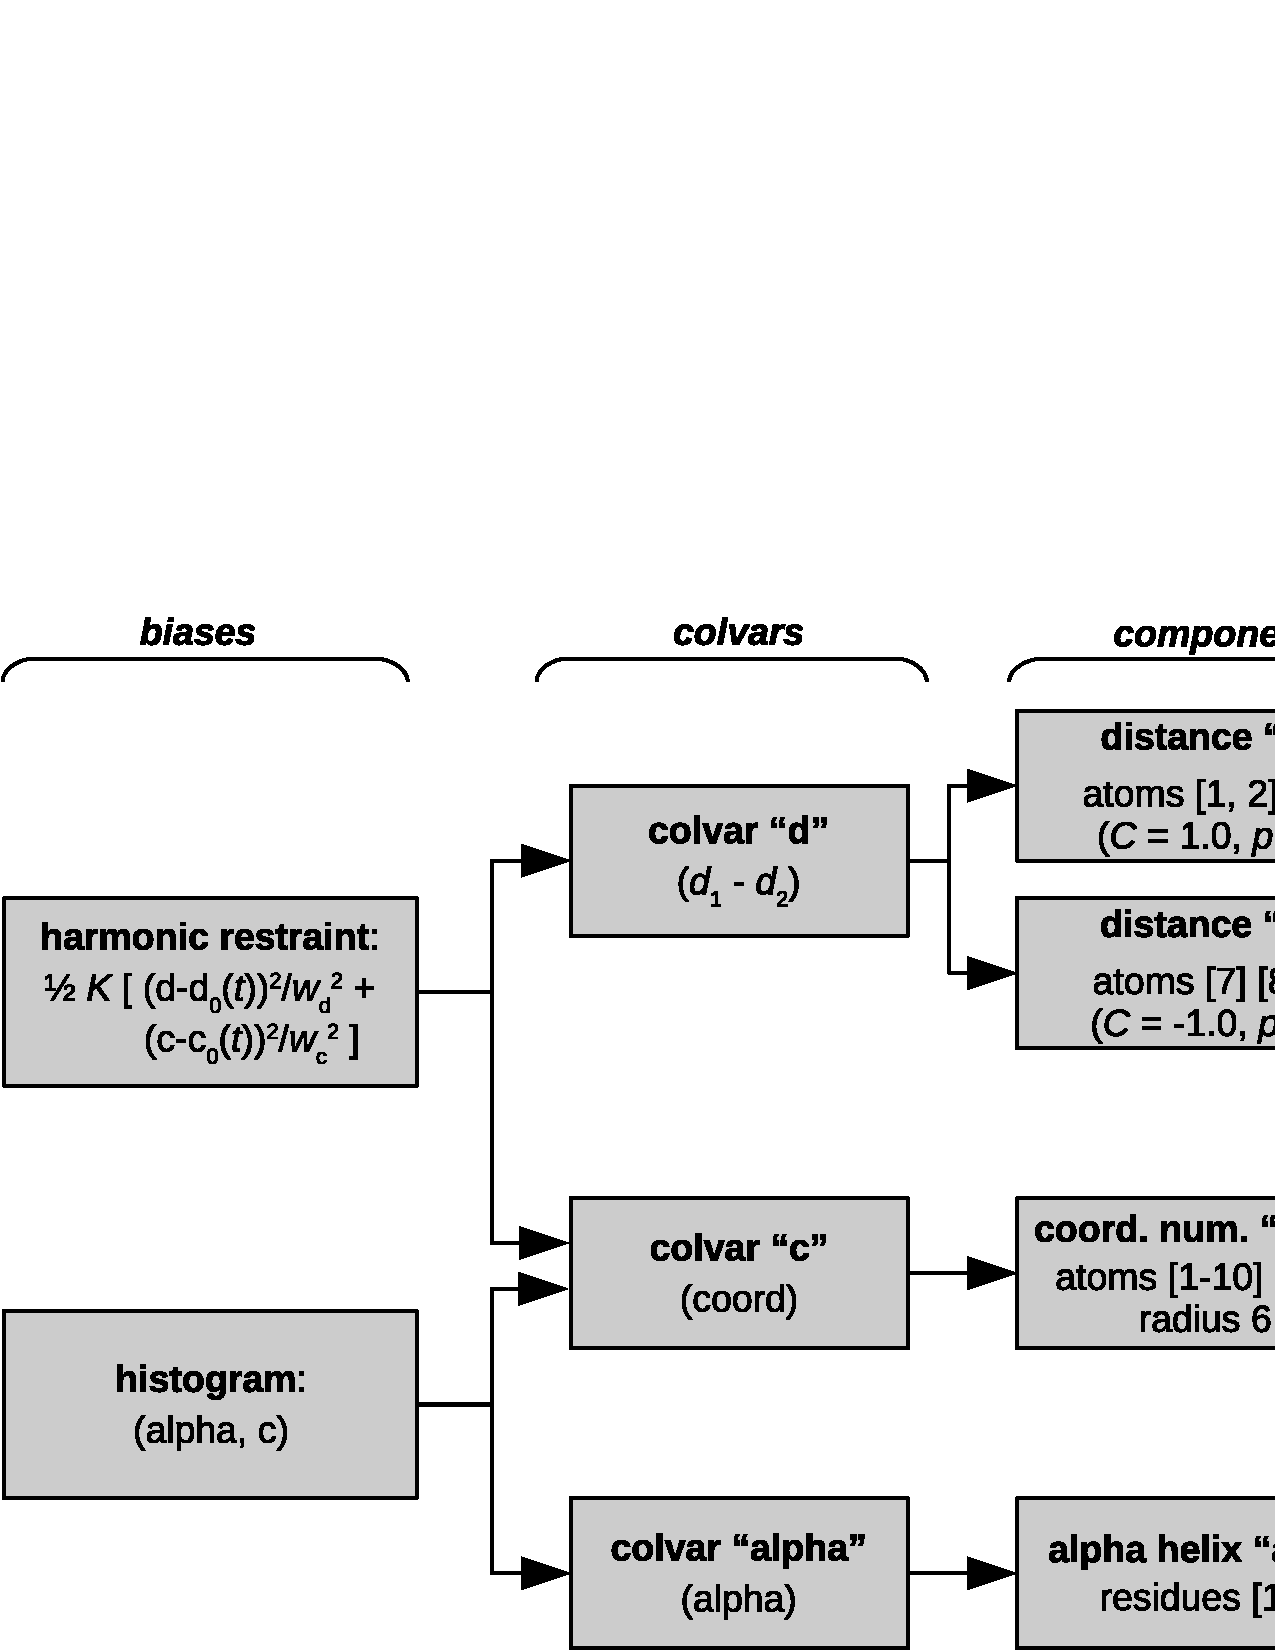
\includegraphics[width=12cm]{figures/colvars_diagram}
  \caption{Example of a collective variables (colvar) configuration.
    The colvar ``$d$'' is defined as the difference between two
    distances, each calculated between the centers of mass of two
    atom groups.  The second colvar ``$c$'' holds the coordination
    number (i.e.~the number of contacts) within a radius of 6~\AA{}
    between two groups.  The third colvar ``alpha'' measures the
    degree of $\alpha$-helicity of the protein segment between
    residues 1 and 10. A moving harmonic restraint is applied to the
    colvars ``$d$'' and ``$c$'', each rescaled by means of width
    parameters $w_{d}$ and $w_{c}$; the centers of the restraint,
    $d_0$ and $c_0$, evolve with the simulation time $t$. The joint
    histogram of ``alpha'' and ``$c$'' is also recorded on-the-fly.}
  \label{fig:colvars_diagram}
\end{figure}


\subsubsection{NAMD parameters}

To enable a colvar calculation, two parameters should be added to the
NAMD configuration file must set (three when restarting a previous
run):

\begin{itemize}
  \setlength{\itemsep}{0.4cm}

\item %
  \NAMDCONFWDEF{%
    colvars}{%
    Enable the collective variables module}{%
    boolean}{%
    \texttt{off}}{%
    If this flag is on, the collective variables module within NAMD is
    executed at each time step; the module requires a separate
    configuration file, to be provided with \texttt{colvarsConfig}.}

\item %
  \NAMDCONF{%
    colvarsConfig}{%
    Configuration file for the collective variables}{%
    UNIX filename}{%
    This file contains the definition of all collective variables and
    their biasing or analysis methods.  It is meant to contain all the
    information needed to \emph{begin} a colvars simulation.
    Additional information is needed instead to \emph{continue} a
    previous run, which is read from the file provided by
    \texttt{colvarsInput}.}

\item %
  \NAMDCONF{%
    colvarsInput}{%
    Input state file for the collective variables}{%
    UNIX filename}{%
    When continuing a previous simulation run, this file contains the
    current state of all collective variables and their biasing
    methods.  Its format is similar to that of \texttt{colvarsConfig},
    but with different keywords.  In normal circumstances, this file
    is written automatically at the end of a NAMD run, and the user
    does not need to edit it.}

\end{itemize}

\subsubsection{Output files}

By default, the collective variables module writes three output
files:
\begin{itemize}

\item a \emph{state file}, named
  \texttt{$<$outputName$>$.colvars.state}; this file is in ASCII
  format, regardless of the value of \texttt{binaryOutput} in the NAMD
  configuration; the name of this file can be provided as
  \texttt{colvarsInput} to continue the simulation in the next run;

\item a \emph{restart file} (equivalent to the state file) is written
  every \texttt{colvarsRestartFrequency} steps, if either
  \texttt{colvarsRestartFrequency} or the NAMD parameter
  \texttt{restartFreq} is defined; its name is
  \texttt{$<$restartName$>$.colvars.state}, and can be given as
  \texttt{colvarsInput} to continue an interrupted run; (provided that
  the coordinates and velocities restart files at the same time step
  are also used);

\item a \emph{trajectory file} is written during the simulation, if
  the colvars module parameter \texttt{colvarsTrajFrequency} is
  greater than 0 (default: 100); its name is
  \texttt{$<$outputName$>$.colvars.traj}; unlike the state file it is
  not needed to restart a simulation, but can be read in for
  post-processing (see~\ref{sec:colvar_acf}).

\end{itemize}

Other output files may be written by specific methods applied to the
colvars (e.g.~by the ABF method, see \ref{sec:colvarbias_abf}, or the
metadynamics method, see \ref{sec:colvarbias_meta}).  Like the colvar
trajectory file, they are needed only for analyzing, not continuing a
simulation.  All such files' names also begin with the prefix
\texttt{$<$outputName$>$}.


\subsubsection{Colvars module configuration file}

Except for the three NAMD keywords listed above (\texttt{colvars},
\texttt{colvarsConfig} and \texttt{colvarsInput}), all the parameters
defining the colvars and their biases are read from the extra input
file (provided by \texttt{colvarsConfig}).  Hence, none of the
keywords described in this and the following sections are available in
the NAMD main configuration.

The syntax of the collective variables configuration file is similar
to that of the NAMD file (\ref{section:configsyntax}), with a few
important differences:
\begin{itemize}
\item certain keywords may have multiple values;
\item a long value (or values) can be distributed across several
  lines, by using curly braces (\texttt{\{} and \texttt{\}}): the
  opening brace (\texttt{\{}) must occur on the same line as the
  keyword, after a space character or any other white space;
\item blocks defined by curly braces may be nested: therefore, the
  values of a keyword (such as \texttt{colvar}) may in turn contain
  simple keywords (such as \texttt{name}) and keywords with other
  blocks (such as \texttt{distance});
\item nested keywords are only meaningful within the parent keyword's
  block, and \emph{not} elsewhere: when the same keyword is available
  within different blocks, it may have different meanings; for every
  keyword documented in the following, the ``parent'' keyword defining
  the context block is indicated in parentheses;
\item certain keywords can be used multiple times even within the same
  context (e.g.~the keyword \texttt{colvar});
\item as in the NAMD configuration, comments can be inserted at any
  point using the hash sign, \texttt{\#};
\item unlike in the NAMD config, the deprecated `\texttt{=}' sign
  between a keyword and its value, is not allowed;
\item Tcl commands and variables are not available;
\item if a keyword requiring a boolean value (\texttt{yes|on|true} or
  \texttt{no|off|false}) is provided without an explicit value, it
  defaults to `\texttt{yes|on|true}'; for example,
  `\texttt{outputAppliedForce}' may be used as shorthand for
  `\texttt{outputAppliedForce on}'.
\end{itemize}

Three global options are available:
\begin{itemize}

\item %
  \NAMDCONFWDEF{%
    colvarsTrajFrequency}{%
    (global) Colvar value trajectory frequency}{%
    positive integer}{%
    \texttt{100}}{%
    The values of each colvar (and any additional quantities which
    have been set to be reported) are written at this frequency to the
    file \texttt{<outputName>.colvars.traj}. If the value is
    \texttt{0}, the trajectory file is not written.  For optimization,
    the output is buffered (as is the NAMD log output in most
    operating systems), but it is synchronized with the disks every
    time the restart file is written.}

\item %
  \NAMDCONFWDEF{%
    colvarsTrajAppend}{%
    (global) Append to trajectory file?}{%
    boolean}{%
    \texttt{off}}{%
    If this flag is enabled, and a file with the same name as the
    trajectory file is already present, new data is appended to that
    file.  Otherwise, a new file is created.  \textbf{Note:} \emph{if
      you're running consecutive simulations with the same
    }\texttt{outputName}\emph{ (e.g.~in FEP calculations), you should
      enable this option to preserve the previous contents of the
      trajectory file}.}

\item %
  \NAMDCONFWDEF{%
    colvarsRestartFrequency}{%
    (global) Colvar module restart frequency}{%
    positive integer}{%
    \texttt{restartFreq}}{%
    Allows to choose a different restart frequency for the collective
    variables module.  Redefining it may be useful to trace the time
    evolution of those few properties which are not written to the
    trajectory file for reasons of disk space.}

\item %
  \NAMDCONFWDEF{%
    analysis}{%
    (global) Turn on run-time statistical analysis }{%
    boolean}{%
    \texttt{off}}{%
    If this flag is enabled, each colvar is instructed to perform
    whatever run-time statistical analysis it is configured to, such as
    correlation functions, or running averages and standard deviations.
    See section~\ref{sec:colvar_acf} for details.}

% \item %
%   \NAMDCONF{%
%     readTrajectory}{%
%     (global, analysis mode) Trajectory file to read}{%
%     UNIX filename}{%
%     If \texttt{analysis} is on, and the colvar module has been
%     compiled as standalone, the values of the colvars is
%     read from this file, as if a regular simulation was going on.  The
%     same configuration as that of the run which produced the trajectory should
%     be used to ensure that data is read properly.}

% \item %
%   \NAMDCONFWDEF{%
%     readBegin}{%
%     (global, analysis mode) Only read frames from this step}{%
%     positive integer}{%
%     \texttt{0}}{%
%     If \texttt{readTrajectory} is defined, only lines starting from
%     this step number are actually loaded by the colvars.}

% \item %
%   \NAMDCONFWDEF{%
%     readEnd}{%
%     (global, analysis mode) Only read frames up to this step}{%
%     positive integer}{%
%     \texttt{0}}{%
%     If \texttt{readTrajectory} is defined, and this number is larger
%     than \texttt{readBegin}, only lines up to and including this
%     step number are actually loaded in the colvars.}

\end{itemize}

The following is a typical configuration file.  The options available
inside the two \texttt{colvar} blocks are documented in
\ref{sec:colvar}.  \texttt{harmonic} defines an harmonic potential,
which is one of the available biases, documented in
\ref{sec:colvarbias}.  \textbf{Note:} \emph{except
}\texttt{colvar}\emph{, none of the keywords below is mandatory}.
\begin{verbatim}
# collective variables config file: two distances

colvarsTrajFrequency 100 # output values every 100 steps

colvar {
  name 1st-colvar # needed to identify the variable

  outputSystemForce yes # report also the system force on this colvar
                        # (in addition to the current value)
  distance {
    group1 {
      atomNumbers 1 2 3 
    }
    group2 {
      atomNumbers 4 5 6 
    }
  }
}

colvar {
  name 2nd-colvar
  ...
}

harmonic {
  name my_pot
  colvars 1st-colvar 2nd-colvar
  centers 3.0 4.0
  forceConstant 5.0
}
\end{verbatim}

In the following, the section \ref{sec:colvar} explains how to define
a colvar.  \ref{sec:cvc} lists the available colvar components;
\ref{sec:cvc_superp} defines how to combine existing components to
create new types of colvars; \ref{sec:colvar_atom_groups} documents
how to define in a compact way \emph{atom groups}, which are used by
most components; \ref{sec:colvar_acf} lists the available option for
runtime statistical analysis of the colvars.

\ref{sec:colvarbias} lists the available methods to perform biased
simulations and multidimensional analysis (ABF, harmonic restraint,
histogram, and metadynamics).


\subsection{Declaring and using collective variables}
\label{sec:colvar}

Each collective variable (colvar) is defined as a combination of one
or more individual quantities, called \emph{components} (see
Figure~\ref{fig:colvars_diagram}).  In most applications, only one is
needed: in this case, the colvar and its component may be identified.

In the configuration file, each colvar is created by the keyword
\texttt{colvar}, followed by its configuration options, usually
between curly braces, \texttt{colvar~\{...\}}.  Each component is
defined within the the \texttt{colvar~\{...\}} block, with a specific
keyword that identifies the functional form: for example,
\texttt{distance \{...\}} defines a component of the type ``distance
between two atom groups''.

To obtain the value of the colvar, $\xi(\mathbf{r})$, its components
$q_{i}(\mathbf{r})$ are summed with the formula:
\begin{equation}
  \label{eq:colvar_combination}
  \xi(\mathbf{r}) = \sum_{i} c_{i} [q_{i}(\mathbf{r})]^{n_{i}}
\end{equation}
where each component appears with a unique coefficient $c_{i}$ (1.0 by
default) the positive integer exponent $n_{i}$ (1 by default).
For information on setting these parameters, see \ref{sec:cvc_superp}.

Each colvar accepts the following parameters:
\begin{itemize}

\item %
  \NAMDCONFWDEF{%
    name}{%
    (\texttt{colvar}) Name of this colvar}{%
    string}{%
    ``\texttt{colvar}'' + numeric id}{%
    The name is an unique case-sensitive string which allows the
    colvar module to identify this colvar unambiguously; it is also
    used in the trajectory file to label to the columns corresponding
    to this colvar.}

\item %
  \NAMDCONFWDEF{%
    width}{%
    (\texttt{colvar}) Typical fluctuation amplitude (or grid
    spacing)}{%
    positive decimal}{%
    1.0}{%
    This number is a user-provided estimate of the typical
    fluctuation amplitude for this collective variable, or conversely,
    the typical width of a local free energy basin.  Typically, twice
    the standard deviation during a very short simulation run can be
    used.  Biasing methods use this parameter for different purposes:
    harmonic restraints (\ref{sec:colvarbias_harmonic}) use it to
    rescale the value of this colvar, the histogram
    (\ref{sec:colvarbias_histogram}) and ABF biases
    (\ref{sec:colvarbias_abf}) interpret it as the grid spacing in the
    direction of this variable, and metadynamics
    (\ref{sec:colvarbias_meta}) uses it to set the width of newly
    added hills.  This number is expressed in the same physical unit
    as the colvar value.}

\item %
  \NAMDCONF{%
    lowerBoundary}{%
    (\texttt{colvar}) Lower boundary of the colvar}{%
    decimal}{%
    Defines the lowest possible value in the domain of values that
    this colvar can access.  It can either be the true lower physical
    boundary (under which the variable is not defined by
    construction), or an arbitrary value set by the user.  Together
    with \texttt{upperBoundary} and \texttt{width}, it provides
    initial parameters to define grids of values for the colvar.  This
    option is not available for those colvars that return non-scalar
    values (i.e.~those based on the components \texttt{distanceDir}
    or \texttt{orientation}).}

\item %
  \NAMDCONF{%
    upperBoundary}{%
    (\texttt{colvar}) Upper boundary of the colvar}{%
    decimal}{%
    Similarly to \texttt{lowerBoundary}, defines the highest possible
    or allowed value.}

\item %
  \NAMDCONFWDEF{%
    expandBoundaries}{%
    (\texttt{colvar}) Allow biases to expand the two boundaries}{%
    boolean}{%
    \texttt{off}}{%
    If defined, biasing and analysis methods may keep their own copies
    of \texttt{lowerBoundary} and \texttt{upperBoundary}, and expand
    them to accommodate values that do not fit in the initial range.
    Currently, this option is used by the metadynamics bias
    (\ref{sec:colvarbias_meta}) to keep all of its hills fully within
    the grid.  \textbf{Note:} \emph{this option cannot be used when
      the initial boundaries already span the full period of a periodic
      colvar}.}

\item %
  \NAMDCONFWDEF{%
    lowerWall}{%
    (\texttt{colvar}) Position of the lower wall}{%
    decimal}{%
    \texttt{lowerBoundary}}{%
    Defines the value below which a lower bounding restraint on the
    colvar is applied, in the form of a ``half-harmonic'' potential.
    It is a good idea to set this value a little higher than
    \texttt{lowerBoundary}.}

\item %
  \NAMDCONF{%
    lowerWallConstant}{%
    (\texttt{colvar}) Lower wall force constant (kcal/mol)}{%
    positive decimal}{%
    If \texttt{lowerWall} or \texttt{lowerBoundary} is defined,
    provides the force constant.  The energy unit of the constant is
    kcal/mol, while the spatial unit is that of the colvar.}

\item %
  \NAMDCONFWDEF{%
    upperWall}{%
    (\texttt{colvar}) Position of the upper wall}{%
    decimal}{%
    \texttt{upperBoundary}}{%
    Similar to \texttt{lowerWall}.  It's a good idea to make it a
    little \emph{lower} than \texttt{upperBoundary}.}

\item %
  \NAMDCONF{%
    upperWallConstant}{%
    (\texttt{colvar}) Upper wall force constant (kcal/mol)}{%
    positive decimal}{%
    Similar to \texttt{lowerWallConstant}.}

\item %
  \NAMDCONFWDEF{%
    outputValue}{%
    (\texttt{colvar}) Output a trajectory for this colvar}{%
    boolean}{%
    \texttt{on}}{%
    If \texttt{colvarsTrajFrequency} is non-zero, the value of this
    colvar is written to the trajectory file every
    \texttt{colvarsTrajFrequency} steps in the column labeled
    ``$<$\texttt{name}$>$''.}

\item %
  \NAMDCONFWDEF{%
    outputVelocity}{%
    (\texttt{colvar}) Output a velocity trajectory for this colvar}{%
    boolean}{%
    \texttt{off}}{%
    If \texttt{colvarsTrajFrequency} is defined, the
    finite-difference calculated velocity of this colvar are written
    to the trajectory file under the label
    ``\texttt{v\_}$<$\texttt{name}$>$''.}

\item %
  \NAMDCONFWDEF{%
    outputSystemForce}{%
    (\texttt{colvar}) Output a system force trajectory for this
    colvar}{%
    boolean}{%
    \texttt{off}}{%
    If \texttt{colvarsTrajFrequency} is defined, and all components
    support its calculation, the total system force on this
    colvar (i.e.~the projection of all interatomic forces
    except constraint forces on this colvar --- see
    equation~(\ref{eq:gradient_vector}) in
    section~\ref{sec:colvarbias_abf}) are written to the trajectory
    file under the label ``\texttt{fs\_}$<$\texttt{name}$>$''.  The
    physical unit for this force is kcal/mol divided by the colvar
    unit.}

\item %
  \NAMDCONFWDEF{%
    outputAppliedForce}{%
    (\texttt{colvar}) Output an applied force trajectory for this
    colvar}{%
    boolean}{%
    \texttt{off}}{%
    If \texttt{colvarsTrajFrequency} is defined, the total force
    applied on this colvar by biases within the colvar module are
    written to the trajectory under the label
    ``\texttt{fa\_}$<$\texttt{name}$>$''.  The physical unit for this
    force is kcal/mol divided by the colvar unit.}

\item %
  \NAMDCONFWDEF{%
    extendedLagrangian}{%
    (\texttt{colvar}) Add extended degree of freedom}{%
    boolean}{%
    \texttt{off}}{%
    Adds a fictitious particle to be coupled to the colvar by a harmonic
    spring. The fictitious mass and the force constant of the coupling
    potential are derived from the parameters \texttt{extendedTimeConstant}
    and \texttt{extendedFluctuation}, described below. Biasing forces on the
    colvar are applied to this fictitious particle, rather than to the
    atoms directly.  This implements the extended Lagrangian formalism
    used in some metadynamics simulations~\cite{Iannuzzi2003}.}

\item %
  \NAMDCONFWDEF{%
    extendedFluctuation}{%
    (\texttt{colvar}) Standard deviation between the colvar and the fictitious
    particle (colvar unit)}{%
    positive decimal}{%
    \texttt{0.2 $\times$ width}}{%
    Defines the spring stiffness for the \texttt{extendedLagrangian}
    mode, by setting the typical deviation between the colvar and the extended
    degree of freedom due to thermal fluctuation.
    The spring force constant is calculated internally as $k_B T / \sigma^2$,
    where  $\sigma$ is the value of \texttt{extendedFluctuation}.}

\item %
  \NAMDCONFWDEF{%
    extendedTimeConstant}{%
    (\texttt{colvar}) Oscillation period of the fictitious particle (fs)}{%
    positive decimal}{%
    \texttt{80.0 $\times$ timestep}}{%
    Defines the inertial mass of the fictitious particle, by setting the
    oscillation period of the harmonic oscillator formed by the fictitious
    particle and the spring. The period
    should be much larger than the MD time step to ensure accurate integration
    of the extended particle's equation of motion.
    The fictitious mass is calculated internally as $k_B T (\tau/2 \pi \sigma)^2$,
    where $\tau$ is the period and $\sigma$ is the typical fluctuation (see above).}

\end{itemize}



\subsubsection{Collective variable components}
\label{sec:cvc}

Each colvar is defined by one or more \emph{components} (typically
only one).  Each component consists of a keyword identifying a
functional form, and a definition block following that keyword,
specifying the atoms involved and any additional parameters (cutoffs,
``reference'' values, \ldots).

The types of the components used in a colvar determine the properties
of that colvar, and which biasing or analysis methods can be applied.
In most cases, the colvar returns a real number, which is computed by
one or more instances of the following components:
\begin{itemize}
\item \texttt{distance}: distance between two groups;
\item \texttt{distanceZ}: projection of a distance vector on an axis;
\item \texttt{distanceXY}: projection of a distance vector on a plane;
\item \texttt{angle}: angle between three groups;
\item \texttt{coordNum}: coordination number between two groups;
\item \texttt{selfCoordNum}: coordination number of atoms within a
  group;
\item \texttt{hBond}: hydrogen bond between two atoms;
\item \texttt{rmsd}: root mean square deviation (RMSD) from a set of
  reference coordinates;
\item \texttt{eigenvector}: projection of the atomic coordinates on a
  vector;
\item \texttt{orientationAngle}: angle of the best-fit rotation from
  a set of reference coordinates;
\item \texttt{tilt}: projection on an axis of the best-fit rotation
  from a set of reference coordinates;
\item \texttt{gyration}: radius of gyration of a group of atoms;
\item \texttt{alpha}: $\alpha$-helix content of a protein segment.
\end{itemize}


\paragraph*{Periodic components.}  The following components returns
real numbers that lie in a periodic interval:
\begin{itemize}
\item \texttt{dihedral}: torsional angle between four groups;
\item \texttt{spinAngle}: angle of rotation around a predefined axis
  in the best-fit from a set of reference coordinates.
\end{itemize}
In certain conditions, \texttt{distanceZ} can also be periodic, namely
when periodic boundary conditions (PBCs) are defined in the simulation
and \texttt{distanceZ}'s axis is parallel to a unit cell vector.

The following keywords can be used within periodic components (and are
illegal elsewhere):
\begin{itemize}
\item %
  \NAMDCONFWDEF{%
    period}{%
    (\texttt{distanceZ}) Period of the component}{%
    positive decimal}{%
    0.0}{%
    Setting this number enables the treatment of \texttt{distanceZ} as
    a periodic component: by default, \texttt{distanceZ} is not
    considered periodic.  The keyword is supported, but irrelevant
    within \texttt{dihedral} or \texttt{spinAngle}, because their
    period is always 360~degrees.}

\item %
  \NAMDCONFWDEF{%
    wrapAround}{%
    (\texttt{distanceZ}, \texttt{dihedral} or \texttt{spinAngle}) Wrap
    periodic variables around this value}{%
    decimal}{%
    0.0}{%
    By default, values of the periodic components are centered around
    zero, ranging from $-P/2$ to $P/2$, where $P$ is the period.
    Setting this number centers the interval around this value.  This
    can be useful for convenience of output, or to set
    \texttt{lowerWall} and \texttt{upperWall} in an order that would
    not otherwise be allowed.}
\end{itemize}
All differences between two values of a periodic colvar are handled
internally using the two periodic images that are least distant
between each other.  Periodic components cannot be summed or
superimposed together with regular ones.


\paragraph*{Non-scalar components.}  When one of the following are
used, the colvar returns a value that is not a scalar number:
\begin{itemize}
\item \texttt{distanceDir}: 3-dimensional unit vector of the distance
  between two groups;
\item \texttt{orientation}: 4-dimensional unit quaternion representing
  the best-fit rotation from a set of reference coordinates.
\end{itemize}
The distance between two 3-dimensional unit vectors is computed as the
angle between them.  The distance between two quaternions is computed
as the angle between the two 4-dimensional unit vectors: because the
orientation represented by $\mathsf{q}$ is the same as the one
represented by $-\mathsf{q}$, distances between two quaternions are
computed considering the closest of the two symmetric images.

Each colvar can only contain one non-scalar component.  Also, binning
on a grid (\texttt{abf}, \texttt{histogram} and \texttt{metadynamics}
with \texttt{useGrids} enabled) is currently not supported for colvars
based on such components.


\paragraph*{Restrictions on certain components.}  In addition to the
type of value returned, components may have other differences.  For
instance, properties like the system force (\texttt{outputSystemForce}
option) can be calculated and used only from certain ones
(\texttt{distance}, \texttt{distanceZ}, \texttt{distanceXY},
\texttt{dihedral}, \texttt{rmsd}, \texttt{eigenvector} and
\texttt{gyration}).  \emph{Note: restrictions only apply to the type
  of an individual colvar; Instead, all of the implemented biasing
  methods can be applied to any number of colvars.}


\paragraph*{Syntax of a component definition.}  Most components make
use of one or more \emph{atom groups}, whose syntax of definition is
by their name followed by a definition block like
\texttt{atoms~\{...\}}, or \texttt{group1~\{...\}} and
\texttt{group2~\{...\}}.  The contents of an atom group block are
described in \ref{sec:colvar_atom_groups}.

In the following, all the available component types are listed, along
with their physical units and the limiting values, if any.  Such
limiting values can be used to define \texttt{lowerBoundary} and
\texttt{upperBoundary} in the parent colvar.


\paragraph*{Component \texttt{distance}: center-of-mass distance between two groups.}
The \texttt{distance \{...\}} block defines a distance component,
between two atom groups, \texttt{group1} and \texttt{group2}.
\begin{itemize}
\item %
  \NAMDCONF{%
    group1}{%
    (\texttt{distance}) First group of atoms}{%
    Block \texttt{group1 \{...\}}}{%
    First group of atoms.}
\item %
  \NAMDCONF{%
    group2}{%
    (\texttt{distance}) Second group of atoms}{%
    Block \texttt{group2 \{...\}}}{%
    Second group of atoms.}
\item %
  \NAMDCONFWDEF{%
    forceNoPBC}{%
    (\texttt{distance}) Calculate absolute rather than minimum-image distance?}{%
    boolean}{%
    \texttt{no}}{%
    By default, in calculations with periodic boundary conditions, the
    \texttt{distance} component returns the distance according to the
    minimum-image convention. If this parameter is set to \texttt{yes},
    PBC will be ignored and the distance between the coordinates as maintained
    internally will be used. This is only useful in a limited number of
    special cases, e.g. to describe the distance between remote points
    of a single macromolecule, which cannot be split across periodic cell
    boundaries, and for which the minimum-image distance might give the
    wrong result because of a relatively small periodic cell.}
\item %
  \NAMDCONFWDEF{%
    oneSiteSystemForce}{%
    (\texttt{distance}) Measure system force on group 1 only?}{%
    boolean}{%
    \texttt{no}}{%
    If this is set to \texttt{yes}, the system force is measured along
    a vector field (see equation~(\ref{eq:gradient_vector}) in
    section~\ref{sec:colvarbias_abf}) that only involves atoms of
    \texttt{group1}.  This option is only useful for ABF, or custom
    biases that compute system forces.  See
    section~\ref{sec:colvarbias_abf} for details.}
\end{itemize}

The value returned is a positive number (in \AA), ranging from $0$
to the largest possible interatomic distance within the chosen
boundary conditions (with PBCs, the minimum image convention is used
unless the \texttt{forceNoPBC} option is set).


\paragraph*{Component \texttt{distanceZ}: projection of a distance vector on an axis.} 
The \texttt{distanceZ~\{...\}} block defines a distance projection
component, which can be seen as measuring the distance between two
groups projected onto an axis, or the position of a group along such
an axis.  The axis can be defined using either one reference group and
a constant vector, or dynamically based on two reference groups.
\begin{itemize}
\item %
  \NAMDCONF{%
    main}{%
    (\texttt{distanceZ, \texttt{distanceXY}}) Main group of atoms}{%
    Block \texttt{main \{...\}}}{%
    Group of atoms whose position $\bm{r}$ is measured.}
\item %
  \NAMDCONF{%
    ref}{%
    (\texttt{distanceZ, \texttt{distanceXY}}) Reference group of
    atoms}{%
    Block \texttt{ref \{...\}}}{%
    Reference group of atoms.  The position of its center of mass is
    noted $\bm{r}_1$ below.}
\item %
  \NAMDCONFWDEF{%
    ref2}{%
    (\texttt{distanceZ, \texttt{distanceXY}}) Secondary reference
    group}{%
    Block \texttt{ref2 \{...\}}}{%
    none}{%
    Optional group of reference atoms, whose position $\bm{r}_2$ can
    be used to define a dynamic projection axis: $\bm{e}=(\| \bm{r}_2
    - \bm{r}_1\|)^{-1} \times (\bm{r}_2 - \bm{r}_1)$.  In this case,
    the origin is $\bm{r}_m = 1/2 (\bm{r}_1+\bm{r}_2)$, and the value
    of the component is $\bm{e} \cdot (\bm{r}-\bm{r}_m)$.}
\item %
  \NAMDCONFWDEF{%
    axis}{%
    (\texttt{distanceZ}, \texttt{distanceXY}) Projection axis (\AA{})}{%
    \texttt{(x, y, z)} triplet}{%
    \texttt{(0.0, 0.0, 1.0)}}{%
    The three components of this vector define (when normalized) a
    projection axis $\bm{e}$ for the distance vector $\bm{r} -
    \bm{r}_1$ joining the centers of groups \texttt{ref} and
    \texttt{main}. The value of the component is then $\bm{e} \cdot
    (\bm{r}-\bm{r}_1)$.  The vector should be written as three
    components separated by commas and enclosed in parentheses.}
\item %
  \NAMDCONFWDEF{%
    forceNoPBC}{%
    (\texttt{distanceZ, distanceXY}) Calculate absolute rather than minimum-image distance?}{%
    boolean}{%
    \texttt{no}}{%
    This parameter has the same meaning as that described above for the \texttt{distance}
    component.}
\item %
  \NAMDCONFWDEF{%
    oneSiteSystemForce}{%
    (\texttt{distanceZ, distanceXY}) Measure system force on group \texttt{main} only?}{%
    boolean}{%
    \texttt{no}}{%
    If this is set to \texttt{yes}, the system force is measured along a
    vector field (see equation~(\ref{eq:gradient_vector}) in
    section~\ref{sec:colvarbias_abf}) that only involves atoms of \texttt{main}.
    This option is only useful for ABF, or custom biases that compute
    system forces.  See section~\ref{sec:colvarbias_abf} for details.}
\end{itemize}
This component returns a number (in \AA{}) whose range is determined
by the chosen boundary conditions.  For instance, if the $z$ axis is
used in a simulation with periodic boundaries, the returned value ranges
between $-b_{z}/2$ and $b_{z}/2$, where $b_{z}$ is the box length
along $z$ (this behavior is disabled if \texttt{forceNoPBC} is set).


\paragraph*{Component \texttt{distanceXY}: modulus of the projection
 of a distance vector on a plane.}
The \texttt{distanceXY~\{...\}} block defines a distance projected on
a plane, and accepts the same keywords as \texttt{distanceZ}, i.e.
\texttt{main}, \texttt{ref}, either \texttt{ref2} or \texttt{axis},
and \texttt{oneSiteSystemForce}.  It returns the norm of the
projection of the distance vector between \texttt{main} and
\texttt{ref} onto the plane orthogonal to the axis.  The axis is
defined using the \texttt{axis} parameter or as the vector joining
\texttt{ref} and \texttt{ref2} (see \texttt{distanceZ} above).


\paragraph*{Component \texttt{distanceDir}: distance unit vector
  between two groups.}  The \texttt{distanceDir~\{...\}} block defines
a distance unit vector component, which accepts the same keywords as
\texttt{distance}: \texttt{group1}, \texttt{group2}, and
\texttt{forceNoPBC}.  It returns a
3-dimensional unit vector $\mathbf{d} = (d_{x}, d_{y}, d_{z})$, with
$|\mathbf{d}| = 1$.  $d_{x}$, $d_{y}$ and $d_{z}$ all lie within the
$[-1:1]$ interval.


\paragraph*{Component \texttt{angle}: angle between three groups.}
The \texttt{angle~\{...\}} block defines an angle, and contains the
three blocks \texttt{group1}, \texttt{group2} and \texttt{group3}, defining
the three groups.  It returns an angle (in degrees) within the
interval $[0:180]$.


\paragraph*{Component \texttt{dihedral}: torsional angle between four groups.}
The \texttt{dihedral~\{...\}} block defines a torsional angle, and
contains the blocks \texttt{group1}, \texttt{group2}, \texttt{group3}
and \texttt{group4}, defining the four groups.  It returns an angle
(in degrees) within the interval $[-180:180]$.  The colvar module
calculates all the distances between two angles taking into account
periodicity.  For instance, reference values for restraints or range
boundaries can be defined by using any real number of choice.
\begin{itemize}
\item \NAMDCONFWDEF{%
    oneSiteSystemForce}{%
    (\texttt{dihedral}) Measure system force on group 1 only?}{%
    boolean}{%
    \texttt{no}}{%
    If this is set to \texttt{yes}, the system force is measured along
    a vector field (see equation~(\ref{eq:gradient_vector}) in
    section~\ref{sec:colvarbias_abf}) that only involves atoms of
    \texttt{group1}.  See section~\ref{sec:colvarbias_abf} for an
    example.}
\end{itemize}


\paragraph*{Component \texttt{coordNum}: coordination number
  between two groups.}  The \texttt{coordNum \{...\}} block defines
a coordination number (or number of contacts), which calculates the
function $(1-(d/d_0)^{n})/(1-(d/d_0)^{m})$, where $d_0$ is the
``cutoff'' distance, and $n$ and $m$ are exponents that can control
its long range behavior and stiffness \cite{Iannuzzi2003}.  This
function is summed over all pairs of atoms in \texttt{group1} and
\texttt{group2}:
\begin{equation}
  \label{eq:cvc_coordNum}
  C (\mathtt{group1}, \mathtt{group2}) \; = \; 
  \sum_{i\in\mathtt{group1}}\sum_{j\in\mathtt{group2}} {
    \frac{1 - (|\mathbf{x}_{i}-\mathbf{x}_{j}|/d_{0})^{n}}{
      1 - (|\mathbf{x}_{i}-\mathbf{x}_{j}|/d_{0})^{m} }
  }
\end{equation}
This colvar component accepts the same keywords as \texttt{distance},
\texttt{group1} and \texttt{group2}.  In addition to them, it
recognizes the following keywords:

\begin{itemize}

\item %
  \NAMDCONFWDEF{%
    cutoff}{%
    (\texttt{coordNum}) ``Interaction'' distance (\AA)}{%
    positive decimal}{%
    4.0}{%
    This number defines the switching distance to define an
    interatomic contact: for $d \ll d_0$, the switching function
    $(1-(d/d_0)^{n})/(1-(d/d_0)^{m})$ is close to 1, at $d = d_0$ it
    has a value of $n/m$ ($1/2$ with the default $n$ and $m$), and at
    $d \gg d_0$ it goes to zero approximately like $d^{m-n}$.  Hence,
    for a proper behavior, $m$ must be larger than $n$.}

\item %
  \NAMDCONFWDEF{%
    expNumer}{%
    (\texttt{coordNum}) Numerator exponent}{%
    positive even integer}{%
    6}{%
    This number defines the $n$ exponent for the switching function.}

\item %
  \NAMDCONFWDEF{%
    expDenom}{%
    (\texttt{coordNum}) Denominator exponent}{%
    positive even integer}{%
    12}{%
    This number defines the $m$ exponent for the switching function.}

\item %
  \NAMDCONFWDEF{%
    cutoff3}{%
    (\texttt{coordNum}) Reference distance vector (\AA)}{%
    ``\texttt{(x, y, z)}'' triplet of positive decimals}{%
    \texttt{(4.0, 4.0, 4.0)}}{%
    The three components of this vector define three different cutoffs
    $d_{0}$ for each direction.  This option is mutually exclusive with
    \texttt{cutoff}.}

\item %
  \NAMDCONFWDEF{%
    group2CenterOnly}{%
    (\texttt{coordNum}) Use only \texttt{group2}'s center of
    mass}{%
    boolean}{%
    \texttt{off}}{%
    If this option is \texttt{on}, only contacts between the atoms in
    \texttt{group1} and the center of mass of \texttt{group2} are
    calculated.  By default, the sum extends over all pairs of
    atoms in \texttt{group1} and \texttt{group2}.}

\end{itemize}

This component returns a dimensionless number, which ranges from
approximately 0 (all interatomic distances much larger than the
cutoff) to $N_{\mathtt{group1}} * N_{\mathtt{group2}}$ (all distances
within the cutoff), or $N_{\mathtt{group1}}$ if
\texttt{group2CenterOnly} is used.  For performance reasons, at least
one of \texttt{group1} and \texttt{group2} should be of limited size
(unless \texttt{group2CenterOnly} is used), because the cost of the
loop over all pairs grows as $N_{\mathtt{group1}} * N_{\mathtt{group2}}$.



\paragraph*{Component \texttt{selfCoordNum}: coordination number
  between atoms within a group.}  The \texttt{selfCoordNum \{...\}} block defines
a coordination number in much the same way as \texttt{coordNum},
but the function is summed over atom pairs within \texttt{group1}:
\begin{equation}
  \label{eq:cvc_selfCoordNum}
  C (\mathtt{group1}) \; = \; 
  \sum_{i\in\mathtt{group1}}\sum_{j > i} {
    \frac{1 - (|\mathbf{x}_{i}-\mathbf{x}_{j}|/d_{0})^{n}}{
      1 - (|\mathbf{x}_{i}-\mathbf{x}_{j}|/d_{0})^{m} }
  }
\end{equation}
The keywords accepted by \texttt{selfCoordNum} are a subset of
those accepted by \texttt{coordNum}, namely \texttt{group1}
(here defining \emph{all} of the atoms to be considered),
\texttt{cutoff}, \texttt{expNumer}, and \texttt{expDenom}.

This component returns a dimensionless number, which ranges from
approximately 0 (all interatomic distances much larger than the
cutoff) to $N_{\mathtt{group1}} * (N_{\mathtt{group1}} - 1) / 2$ (all
distances within the cutoff).  For performance reasons,
\texttt{group1} should be of limited size, because the cost of the
loop over all pairs grows as $N_{\mathtt{group1}}^2$.



\paragraph*{Component \texttt{hBond}: hydrogen bond between two
  atoms.}  The \texttt{hBond \{...\}} block defines a hydrogen
bond, implemented as a coordination number (eq.~\ref{eq:cvc_coordNum})
between the donor and the acceptor atoms.  Therefore, it accepts the
same options \texttt{cutoff} (with a different default value of
3.3~\AA{}), \texttt{expNumer} (with a default value of 6) and
\texttt{expDenom} (with a default value of 8).  Unlike
\texttt{coordNum}, it requires two atom numbers, \texttt{acceptor} and
\texttt{donor}, to be defined.  It returns an adimensional number,
with values between 0 (acceptor and donor far outside the cutoff
distance) and 1 (acceptor and donor much closer than the cutoff).


\paragraph*{Component \texttt{rmsd}: root mean square displacement
  (RMSD) with respect to a reference structure.}  The block
\texttt{rmsd~\{...\}} defines the root mean square replacement
(RMSD) of a group of atoms with respect to a reference structure.  For
each set of coordinates $\{ \mathbf{x}_1(t), \mathbf{x}_2(t), \ldots
\mathbf{x}_N(t) \}$, the colvar component \texttt{rmsd} calculates the
optimal rotation
$U^{\{\mathbf{x}_{i}(t)\}\rightarrow\{\mathbf{x}_{i}^{\mathrm{(ref)}}\}}$
that best superimposes the coordinates $\{\mathbf{x}_{i}(t)\}$ onto a
set of reference coordinates $\{\mathbf{x}_{i}^{\mathrm{(ref)}}\}$.
Both the current and the reference coordinates are centered on their
centers of geometry, $\mathbf{x}_{\mathrm{cog}}(t)$ and
$\mathbf{x}_{\mathrm{cog}}^{\mathrm{(ref)}}$.  The root mean square
displacement is then defined as:
\begin{equation}
  \label{eq:cvc_rmsd}
  { \mathrm{RMSD}(\{\mathbf{x}_{i}(t)\},
    \{\mathbf{x}_{i}^{\mathrm{(ref)}}\}) } \; = \; \sqrt{
    \frac{1}{N} \sum_{i=1}^{N} \left|
      U
      \left(\mathbf{x}_{i}(t) - \mathbf{x}_{\mathrm{cog}}(t)\right) -
      \left(\mathbf{x}_{i}^{\mathrm{(ref)}} -
        \mathbf{x}_{\mathrm{cog}}^{\mathrm{(ref)}} \right) \right|^{2} }
\end{equation}
The optimal rotation
$U^{\{\mathbf{x}_{i}(t)\}\rightarrow\{\mathbf{x}_{i}^{\mathrm{(ref)}}\}}$
is calculated within the formalism developed in
reference~\cite{Coutsias2004}, which guarantees a continuous
dependence of
$U^{\{\mathbf{x}_{i}(t)\}\rightarrow\{\mathbf{x}_{i}^{\mathrm{(ref)}}\}}$
with respect to $\{\mathbf{x}_{i}(t)\}$.  The options for \texttt{rmsd}
are:
\begin{itemize}

\item %
  \NAMDCONF{%
    atoms}{%
    (\texttt{rmsd}) Atom group}{%
    \texttt{atoms~\{...\}} block}{%
    Defines the group of atoms of which the RMSD should be calculated.}

\item %
  \NAMDCONF{%
    refPositions}{%
    (\texttt{rmsd}) Reference coordinates}{%
    space-separated list of \texttt{(x, y, z)} triplets}{%
    This option (mutually exclusive with \texttt{refPositionsFile})
    sets the reference coordinates to be compared with.  The list
    should be as long as the atom group \texttt{atoms}.  This option
    is independent from that with the same keyword within the
    \texttt{atoms~\{...\}} block.}

\item %
  \NAMDCONF{%
    refPositionsFile}{%
    (\texttt{rmsd}) Reference coordinates file}{%
    UNIX filename}{%
    This option (mutually exclusive with \texttt{refPositions}) sets
    the PDB file name for the reference coordinates to be compared
    with.  The format is the same as that provided by
    \texttt{refPositionsFile} within an atom group definition,
    but the two options function independently. Note that as a rule,
    \texttt{rotateReference} and associated keywords should NOT
    be used within the atom group \texttt{atoms} of an
    \texttt{rmsd} component.
    }

\item %
  \NAMDCONF{%
    refPositionsCol}{%
    (\texttt{rmsd}) PDB column to use}{%
    \texttt{X}, \texttt{Y}, \texttt{Z}, \texttt{O} or \texttt{B}}{%
    If \texttt{refPositionsFile} is defined, and the file contains
    all the atoms in the topology, this option may be povided to
    set which PDB field will be
    used to select the reference coordinates for \texttt{atoms}.
  }

\item %
  \NAMDCONF{%
    refPositionsColValue}{%
    (\texttt{rmsd}) Value in the PDB column}{%
    positive decimal}{%
    If defined, this value identifies in the PDB column
    \texttt{refPositionsCol} of the file \texttt{refPositionsFile}
    which atom positions are to be read.  Otherwise, all positions
    with a non-zero value will be read.
  }

\end{itemize}
This component returns a positive real number (in \AA).


\paragraph*{Component \texttt{eigenvector}: projection of the atomic
  coordinates on a vector.}  The block
\texttt{eigenvector~\{...\}} defines the projection of the coordinates
of a group of atoms (or more precisely, their deviations from the
reference coordinates) onto a vector in $\mathbb{R}^{3n}$, where $n$ is the
number of atoms in the group. The computed quantity is the
total projection:
\begin{equation}
  \label{eq:cvc_eigenvector}
  { p(\{\mathbf{x}_{i}(t)\},
    \{\mathbf{x}_{i}^{\mathrm{(ref)}}\}) } \; = \; {
    \left(\sum_{i=1}^{n}\mathbf{v}_{i}^{2}\right)^{-1} \sum_{i=1}^{n} 
    \mathbf{v}_{i} \cdot
    \left(U(\mathbf{x}_{i}(t) - \mathbf{x}_{\mathrm{cog}}(t)) -
      (\mathbf{x}_{i}^{\mathrm{(ref)}} -
      \mathbf{x}_{\mathrm{cog}}^{\mathrm{(ref)}}) \right)\mathrm{,} }
\end{equation}
where, as in the \texttt{rmsd} component, $U$ is the optimal rotation
matrix, $\mathbf{x}_{\mathrm{cog}}(t)$ and
$\mathbf{x}_{\mathrm{cog}}^{\mathrm{(ref)}}$ are the centers of
geometry of the current and reference positions respectively, and
$\mathbf{v}_{i}$ are the components of the vector for each atom.
Example choices for $(\mathbf{v}_{i})$ are an eigenvector
of the covariance matrix (essential mode), or a normal
mode of the system.  It is assumed that $\sum_{i}\mathbf{v}_{i} = 0$:
otherwise, the colvars module centers the $\mathbf{v}_{i}$
automatically when reading them from the configuration.

As in the \texttt{rmsd} component, available options are
\texttt{atoms}, \texttt{refPositions} or \texttt{refPositionsFile},
\texttt{refPositionsCol} and \texttt{refPositionsColValue}.  In
addition, the following are recognized:
\begin{itemize}

\item %
  \NAMDCONF{%
    vector}{%
    (\texttt{eigenvector}) Vector components}{%
    space-separated list of \texttt{(x, y, z)} triplets}{%
    This option (mutually exclusive with \texttt{vectorFile})
    sets the values of the vector components.}

\item %
  \NAMDCONF{%
    vectorFile}{%
    (\texttt{eigenvector}) PDB file containing vector components}{%
    UNIX filename}{%
    This option (mutually exclusive with \texttt{vector}) sets the
    name of a PDB file where the vector components will be read from the
    X, Y, and Z fields.
    \textbf{Note:} \emph{The PDB file has limited precision and fixed
      point numbers: in some cases, the vector may not be
      accurately represented, and }\texttt{vector}\emph{ should be
      used instead.}}

\item %
  \NAMDCONF{%
    vectorCol}{%
    (\texttt{eigenvector}) PDB column used to tag participating atoms}{%
    \texttt{O} or \texttt{B}}{%
    Analogous to \texttt{atomsCol}.}

\item %
  \NAMDCONF{%
    vectorColValue}{%
    (\texttt{eigenvector}) Value used to tag participating atoms in the PDB file}{%
    positive decimal}{%
    Analogous to \texttt{atomsColValue}.}

\end{itemize}
This component returns a number (in \AA), whose value ranges between
the smallest and largest absolute positions in the unit cell during
the simulations (see also \texttt{distanceZ}).  Due to the
normalization in eq.~\ref{eq:cvc_eigenvector}, this range does not
depend on the number of atoms involved.


\paragraph*{Component \texttt{gyration}: radius of gyration of a group
  of atoms.}  The block \texttt{gyration~\{...\}} defines the
parameters for calculating the radius of gyration of a group of atomic
positions $\{ \mathbf{x}_1(t), \mathbf{x}_2(t), \ldots \mathbf{x}_N(t)
\}$ with respect to their center of geometry,
$\mathbf{x}_{\mathrm{cog}}(t)$:
\begin{equation}
  \label{eq:colvar_gyration}
  R_{\mathrm{gyr}} \; = \; \sqrt{ \frac{1}{N}
    \sum_{i=1}^{N} \left|\mathbf{x}_{i}(t) -
      \mathbf{x}_{\mathrm{cog}}(t)\right|^{2} }
\end{equation}
This component must contain one \texttt{atoms~\{...\}} block to
define the atom group, and returns a positive number, expressed in
\AA{}.


\paragraph*{Component \texttt{orientation}: orientation from reference
  coordinates.}  The block \texttt{orientation~\{...\}} returns the
same optimal rotation used in the \texttt{rmsd} component to
superimpose the coordinates $\{\mathbf{x}_{i}(t)\}$ onto a set of
reference coordinates $\{\mathbf{x}_{i}^{\mathrm{(ref)}}\}$.  Such
component returns a four dimensional vector $\mathsf{q} = (q_0, q_1,
q_2, q_3)$, with $\sum_{i} q_{i}^{2} = 1$; this \emph{quaternion}
expresses the optimal rotation $\{\mathbf{x}_{i}(t)\} \rightarrow
\{\mathbf{x}_{i}^{\mathrm{(ref)}}\}$ according to the formalism in
reference~\cite{Coutsias2004}.  The quaternion $(q_0, q_1, q_2, q_3)$
can also be written as $\left(\cos(\theta/2), \,
  \sin(\theta/2)\mathbf{u}\right)$, where $\theta$ is the angle and
$\mathbf{u}$ the normalized axis of rotation; for example, a rotation
of 90$^{\circ}$ around the $z$ axis should be expressed as
``\texttt{(0.707, 0.0, 0.0, 0.707)}''.  The script
\texttt{quaternion2rmatrix.tcl} provides Tcl functions for converting
to and from a $4\times{}4$ rotation matrix in a format suitable for
usage in VMD.

The component accepts all the options of \texttt{rmsd}:
\texttt{atoms}, \texttt{refPositions}, \texttt{refPositionsFile} and
\texttt{refPositionsCol}, in addition to:

\begin{itemize}

\item %
  \NAMDCONFWDEF{%
    closestToQuaternion}{%
    (\texttt{orientation}) Reference rotation}{%
    ``\texttt{(q0, q1, q2, q3)}'' quadruplet}{%
    \texttt{(1.0, 0.0, 0.0, 0.0)} (``null'' rotation)}{%
    Between the two equivalent quaternions $(q_0, q_1, q_2, q_3)$ and
    $(-q_0, -q_1, -q_2, -q_3)$, the closer to \texttt{(1.0, 0.0, 0.0,
      0.0)} is chosen.  This simplifies the visualization of the
    colvar trajectory when samples values are a smaller subset of all
    possible rotations.  \textbf{Note:} \emph {this only affects the
      output, never the dynamics}.}

\end{itemize}

\textbf{Hint: stopping the rotation of a protein.}  To stop the
rotation of an elongated macromolecule in solution (and use an
anisotropic box to save water molecules), it is possible to define a
colvar with an \texttt{orientation} component, and restrain it throuh
the \texttt{harmonic} bias around the identity rotation, \texttt{(1.0,
  0.0, 0.0, 0.0)}.  Only the overall orientation of the macromolecule
is affected, and \emph{not} its internal degrees of freedom.  The user
should also take care that the macromolecule is composed by a single
chain, or disable \texttt{wrapAll} otherwise.


\paragraph*{Component \texttt{orientationAngle}: angle of rotation
  from reference coordinates.}  The block
\texttt{orientationAngle~\{...\}} accepts the same options as
\texttt{rmsd} and \texttt{orientation} (\texttt{atoms},
\texttt{refPositions}, \texttt{refPositionsFile} and
\texttt{refPositionsCol}), but it returns instead the angle of
rotation $\omega$ between the current and the reference positions.
This angle is expressed in degrees within the range
[0$^{\circ}$:180$^{\circ}$].




\paragraph*{Component \texttt{alpha}: $\alpha$-helix content of a
  protein segment.}  The block \texttt{alpha~\{...\}} defines the
parameters to calculate the helical content of a segment of protein
residues.  The $\alpha$-helical content across the $N+1$ residues
$N_{0}$ to $N_{0}+N$ is calculated by the formula:
\begin{eqnarray}
  \label{eq:colvars_alpha}
  { 
    \alpha\left(
      \mathrm{C}_{\alpha}^{(N_{0})},
      \mathrm{O}^{(N_{0})},
      \mathrm{C}_{\alpha}^{(N_{0}+1)},
      \mathrm{O}^{(N_{0}+1)},
      \ldots
      \mathrm{N}^{(N_{0}+5)},
      \mathrm{C}_{\alpha}^{(N_{0}+5)},
      \mathrm{O}^{(N_{0}+5)},
      \ldots
      \mathrm{N}^{(N_{0}+N)},
      \mathrm{C}_{\alpha}^{(N_{0}+N)}
    \right)
  } \; = \; \; \; \; \\ \; \; \; \; {
    \nonumber
    \frac{1}{2(N-2)} 
    \sum_{n=N_{0}}^{N_{0}+N-2}
    \mathrm{angf}\left(
        \mathrm{C}_{\alpha}^{(n)},
        \mathrm{C}_{\alpha}^{(n+1)},
        \mathrm{C}_{\alpha}^{(n+2)}\right)
  } \; + \; {
    \frac{1}{2(N-4)} 
    \sum_{n=N_{0}}^{N_{0}+N-4}
    \mathrm{hbf}\left(
      \mathrm{O}^{(n)},
      \mathrm{N}^{(n+4)}\right) \mathrm{,}
  } \\
\end{eqnarray}
where the score function for the $\mathrm{C}_{\alpha} -
\mathrm{C}_{\alpha} - \mathrm{C}_{\alpha}$ angle is defined as: 
\begin{equation}
  \label{eq:colvars_alpha_Calpha}
  {
    \mathrm{angf}\left(
      \mathrm{C}_{\alpha}^{(n)},
      \mathrm{C}_{\alpha}^{(n+1)},
      \mathrm{C}_{\alpha}^{(n+2)}\right)
  } \; = \; {
    \frac{1 - \left(\theta(
        \mathrm{C}_{\alpha}^{(n)},
        \mathrm{C}_{\alpha}^{(n+1)},
        \mathrm{C}_{\alpha}^{(n+2)}) -
        \theta_{0}\right)^{2} /
      \left(\Delta\theta_{\mathrm{tol}}\right)^{2}}{
      1 - \left(\theta(
        \mathrm{C}_{\alpha}^{(n)},
        \mathrm{C}_{\alpha}^{(n+1)},
        \mathrm{C}_{\alpha}^{(n+2)}) -
        \theta_{0}\right)^{4} /
      \left(\Delta\theta_{\mathrm{tol}}\right)^{4}} \mathrm{,}
  }
\end{equation}
and the score function for the $\mathrm{O}^{(n)} \leftrightarrow
\mathrm{N}^{(n+4)}$ hydrogen bond is defined through a \texttt{hBond}
colvar component on the same atoms.  The options recognized within the
\texttt{alpha~\{...\}} block are:
\begin{itemize}

\item %
  \NAMDCONF{%
    residueRange}{%
    (\texttt{alpha}) Potential $\alpha$-helical residues}{%
    ``$<$Initial residue number$>$-$<$Final residue number$>$''}{%
    This option specifies the range of residues on which this
    component should be defined.  The colvar module looks for the
    atoms within these residues named ``\texttt{CA}'', ``\texttt{N}''
    and ``\texttt{O}'', and raises an error if any of those atoms is
    not found.}

\item %
  \NAMDCONF{%
    psfSegID}{%
    (\texttt{alpha}) PSF segment identifier}{%
    string (max 4 characters)}{%
    This option sets the PSF segment identifier for the residues
    specified in \texttt{residueRange}.  This option need not be
    provided when non-PSF topologies are used by NAMD.}


\item %
  \NAMDCONFWDEF{%
    hBondCoeff}{%
    (\texttt{alpha}) Coefficient for the hydrogen bond term}{%
    positive between 0 and 1}{%
    0.5}{%
    This number specifies the contribution to the total value from the
    hydrogen bond terms.  0 will disable the hydrogen bond terms, 1
    will disable the angle terms.}

\item %
  \NAMDCONFWDEF{%
    angleRef}{%
    (\texttt{alpha}) Reference $\mathrm{C}_{\alpha} -
    \mathrm{C}_{\alpha} - \mathrm{C}_{\alpha}$ angle}{%
    positive decimal}{%
    88$^{\circ}$}{%
    This option sets the reference angle used in the score function
    (\ref{eq:colvars_alpha_Calpha}).}

\item %
  \NAMDCONFWDEF{%
    angleTol}{%
    (\texttt{alpha}) Tolerance in the $\mathrm{C}_{\alpha} -
    \mathrm{C}_{\alpha} - \mathrm{C}_{\alpha}$ angle}{%
    positive decimal}{%
    15$^{\circ}$}{%
    This option sets the angle tolerance used in the score function
    (\ref{eq:colvars_alpha_Calpha}).}

\item %
  \NAMDCONFWDEF{%
    hBondCutoff}{%
    (\texttt{alpha}) Hydrogen bond cutoff}{%
    positive decimal}{%
    3.3~\AA{}}{%
    Equivalent to the \texttt{cutoff} option in the \texttt{hBond}
    component.}

\item %
  \NAMDCONFWDEF{%
    hBondExpNumer}{%
    (\texttt{alpha}) Hydrogen bond numerator exponent}{%
    positive integer}{%
    6}{%
    Equivalent to the \texttt{expNumer} option in the \texttt{hBond}
    component.}

\item %
  \NAMDCONFWDEF{%
    hBondExpDenom}{%
    (\texttt{alpha}) Hydrogen bond denominator exponent}{%
    positive integer}{%
    8}{%
    Equivalent to the \texttt{expDenom} option in the \texttt{hBond}
    component.}

\end{itemize}

This component returns positive values, always comprised between 0
(lowest $\alpha$-helical score) and 1 (highest $\alpha$-helical
score).


\subsubsection{Linear and polynomial combinations of components}
\label{sec:cvc_superp}
Any set of components can be combined within a colvar, provided that
they return the same type of values (scalar, unit vector, vector, or
quaternion).  By default, the colvar is the sum of its components.
Linear or polynomial combinations (following
equation~(\ref{eq:colvar_combination})) can be obtained by setting the
following parameters, which are common to all components:
\begin{itemize}
\item %
  \NAMDCONFWDEF{%
    componentCoeff}{%
    (any component) Coefficient of this component in the colvar}{%
    decimal}{%
    \texttt{1.0}}{%
    Defines the coefficient by which this component is multiplied
    (after being raised to \texttt{componentExp}) before being added
    to the sum.}

\item %
  \NAMDCONFWDEF{%
    componentExp}{%
    (any component) Exponent of this component in the colvar}{%
    integer}{%
    \texttt{1}}{%
    Defines the power at which the value of this component is raised
    before being added to the sum.  When this exponent is
    different than 1 (non-linear sum), system forces and the Jacobian
    force are not available, making the colvar unsuitable for ABF calculations.}
\end{itemize}

\textbf{Example:} To define the \emph{average} of a colvar across
different parts of the system, simply define within the same colvar
block a series of components of the same type (applied to different
atom groups), and assign to each component a \texttt{componentCoeff}
of $1/N$.


\subsubsection{Defining atom groups}
\label{sec:colvar_atom_groups}
Each component depends on one or more \emph{atom groups}, which can be
defined by different methods in the configuration file.  Each atom
group block is initiated by the name of the group itself within the
component block, followed by the instructions to the colvar module on
how to select the atoms involved.  Here is an example configuration,
for an atom group called \texttt{myatoms}, which makes use of the most
common keywords:
\begin{verbatim}
# atom group definition
myatoms {
  # add atoms 1, 2 and 3 to this group (note: numbers start from 1)
  atomNumbers {
     1 2 3
  }
  # add all the atoms with occupancy 2 in the file atoms.pdb
  atomsFile             atoms.pdb
  atomsCol              O
  atomsColValue         2.0
  # add all the C-alphas within residues 11 to 20 of segments "PR1" and "PR2"
  psfSegID              PR1 PR2
  atomNameResidueRange  CA 11-20
  atomNameResidueRange  CA 11-20
}
\end{verbatim}

For any atom group, the available options are:
\begin{itemize}

\item %
  \NAMDCONF{%
    atomNumbers}{%
    (atom group) List of atom numbers}{%
    space-separated list of positive integers}{%
    This option adds to the group all the atoms whose numbers are in
    the list.  \emph{Atom numbering starts from 1.}
  }

\item %
  \NAMDCONF{%
    atomNumbersRange}{%
    (atom group) Atoms within a number range}{%
    $<$Starting number$>$-$<$Ending number$>$}{%
    This option adds to the group all the atoms whose numbers are
    within the range specified.  It can be used multiple times for the
    same group.  Atom numbering starts from 1.  May be repeated.
  }

\item %
  \NAMDCONF{%
    atomNameResidueRange}{%
    (atom group) Named atoms within a range of residue numbers}{%
    $<$Atom name$>$ $<$Starting residue$>$-$<$Ending residue$>$}{%
    This option adds to the group all the atoms with the provided
    name, within residues in the given range.  May be repeated for as
    many times as the values of \texttt{psfSegID}.}

\item %
  \NAMDCONF{%
    psfSegID}{%
    (atom group) PSF segment identifier}{%
    space-separated list of strings (max 4 characters)}{%
    This option sets the PSF segment identifier for of
    \texttt{atomNameResidueRange}.  Multiple values can be provided,
    which can correspond to different instances of
    \texttt{atomNameResidueRange}, in the order of their occurrence.
    This option is not needed when non-PSF topologies are used by
    NAMD.}

\item %
  \NAMDCONF{%
    atomsFile}{%
    (atom group) PDB file name for atom selection}{%
    string}{%
    This option selects atoms from the PDB file provided and adds them
    to the group according to the value in the column
    \texttt{atomsCol}.  \textbf{Note:} \emph{the set of atoms PDB file
    provided must match the topology}.}

\item %
  \NAMDCONF{%
    atomsCol}{%
    (atom group) PDB column to use for the selection}{%
    \texttt{X}, \texttt{Y}, \texttt{Z}, \texttt{O} or \texttt{B}}{%
    This option specifies which column in \texttt{atomsFile} is used
    to determine the atoms to be included in the group.
  }

\item %
  \NAMDCONF{%
    atomsColValue}{%
    (atom group) Value in the PDB column}{%
    positive decimal}{%
    If defined, this value in \texttt{atomsCol} identifies of
    \texttt{atomsFile} which atoms are to be read; otherwise, all
    atoms with a non-zero value will be read.
  }

\item %
  \NAMDCONF{%
    dummyAtom}{%
    (atom group) Dummy atom position (\AA{})}{%
    \texttt{(x, y, z)} triplet}{%
    This option makes the group a virtual particle at a fixed position
    in space.  This is useful e.g.~to make colvar components that
    normally calculate functions of the group's center of mass use an
    absolute reference position.  If specified, \texttt{disableForces}
    is also turned on, the center of mass position is \texttt{(x, y,
    z)} and zero velocities and system forces are reported.}

\item %
  \NAMDCONFWDEF{%
    centerReference}{%
    (atom group) Ignore the translations of this group}{%
    boolean}{%
    \texttt{off}}{%
    If this option is \texttt{on}, the center of geometry of this
    group is centered on a reference frame, determined either by
    \texttt{refPositions} or \texttt{refPositionsFile}.  This
    transformation occurs \emph{before} any colvar component has
    access to the coordinates of the group: hence, only the recentered
    coordinates are available to the colvars.  \textbf{Note}:
    \emph{the derivatives of the colvars with respect to the
      translation are usually neglected (except by
    }\texttt{rmsd}\emph{ and }\texttt{eigenvector}\emph{)}.}

\item %
  \NAMDCONFWDEF{%
    rotateReference}{%
    (atom group) Ignore the rotations of this group}{%
    boolean}{%
    \texttt{off}}{%
    If this option is \texttt{on}, this group is rotated around its
    center of geometry, to optimally superimpose to the positions
    given by \texttt{refPositions} or \texttt{refPositionsFile}.  This
    is done before recentering the group, if \texttt{centerReference}
    is also defined.  The algorithm used is the same employed in the
    \texttt{orientation} colvar component \cite{Coutsias2004}.  Forces
    applied by the colvars to this group are rotated back to the
    original frame prior being applied.  \textbf{Note}: \emph{the
      derivatives of the colvars with respect to the rotation are
      usually neglected (except by }\texttt{rmsd}\emph{ and
    }\texttt{eigenvector}\emph{)}.}

\item %
  \NAMDCONF{%
    refPositions}{%
    (atom group) Reference positions (\AA)}{%
    space-separated list of \texttt{(x, y, z)} triplets}{%
    If either \texttt{centerReference} or \texttt{rotateReference} is
    \texttt{on}, these coordinates are used to determine the center of
    mass translation and the optimal rotation, respectively.  In the
    latter case, the list must also be of the same length as this atom
    group.}

\item %
  \NAMDCONF{%
    refPositionsFile}{%
    (atom group) File with reference positions}{%
    UNIX filename}{%
    If either \texttt{centerReference} or \texttt{rotateReference} is
    \texttt{on}, the coordinates from this file are used to determine
    the center of geometry translation and the optimal rotation between
    them and the current coordinates of the group.  This file can
    either \emph{i)} contain as many atoms as the group (in which case
    all of the \texttt{ATOM} records are read) or \emph{ii)} a larger
    number of atoms. In the second case, coordinates will be selected either
    according to flags in column \texttt{refPositionsCol}, or, if that
    parameter is not specified, by index, using the list of atom indices
    belonging to the atom group. In a typical application, a PDB file
    containing both atom flags and reference coordinates is prepared, and 
    provided as both \texttt{atomsFile} and \texttt{refPositionsFile},
    while the flag column is passed to \texttt{atomsCol} and
    \texttt{refPositionsCol}.}

\item %
  \NAMDCONF{%
    refPositionsCol}{%
    (atom group) Column to use in the PDB file}{%
    \texttt{X}, \texttt{Y}, \texttt{Z}, \texttt{O} or \texttt{B}}{%
    Like \texttt{atomsCol} for \texttt{atomsFile}, indicates which
    column to use to identify the atoms in \texttt{refPositionsFile}.
    If not specified, atoms are selected by index, based on the
    atom group definition.}

\item %
  \NAMDCONF{%
    refPositionsColValue}{%
    (atom group) Value in the PDB column}{%
    positive decimal}{%
    Analogous to \texttt{atomsColValue}, but applied to
    \texttt{refPositionsCol}.}

\item %
  \NAMDCONFWDEF{%
    refPositionsGroup}{%
    (atom group) Use an alternate group do perform roto-translational
    fitting}{%
    Block \texttt{refPositionsGroup \{ ... \}}}{%
    This group itself}{%
    If either \texttt{centerReference} or \texttt{rotateReference} is
    defined, this keyword allows to define an additional atom group,
    which is used instead of the current one to calculate the
    translation or the rotation to the reference positions.  For
    example, it is possible to use all the backbone heavy atoms of a
    protein to set the reference frame, but only involve a more
    localized group in the colvar's definition.}

\item %
  \NAMDCONFWDEF{%
    disableForces}{%
    (atom group) Don't apply colvar forces to this group}{%
    boolean}{%
    \texttt{off}}{%
    If this option is \texttt{on}, all the forces applied from the
    colvars to the atoms in this group are ignored.  The applied
    forces on each colvar are still written to the trajectory file, if
    requested.  In some cases it may be desirable to use this option
    in order not to perturb the motion of certain atoms.
    \textbf{Note:} \emph{when used, the biasing forces are not applied
      uniformly: a non-zero net force or torque to the system is
      generated, which may lead to undesired translations or rotations
      of the system.}
  }

\end{itemize}

\textbf{Note:} to minimize the length of the NAMD standard output,
messages in the atom group's configuration are not echoed by default.
This can be overcome by the boolean keyword \texttt{verboseOutput}
within the group.


\paragraph*{Recommendations for using atom groups.}  When defining the
atom groups for a collective variable, these guidelines should be
followed to avoid inconsistencies and performance losses:

\begin{itemize}

\item In simulations with periodic boundary conditions, NAMD maintains
  the coordinates of all the atoms within a molecule contiguous to
  each other (i.e.~there are no spurious ``jumps'' in the molecular
  bonds).  The colvar module relies on this when calculating a group's
  center of mass, but this condition may fail when the group spans
  different molecules: in that case, writing the NAMD output files
  \texttt{wrapAll} or \texttt{wrapWater} could produce wrong results
  when a simulation run is continued from a previous one.  There are
  however cases in which \texttt{wrapAll} or \texttt{wrapWater} can be
  safely applied:
  \begin{enumerate}
  \item[\emph{i)}] the group has only one atom;
  \item[\emph{ii)}] it has all its atoms within the same molecule;
  \item[\emph{iii)}] it is used by a colvar component which does not
    access its center of mass and uses instead only interatomic
    distances (\texttt{coordNum}, \texttt{hBond}, \texttt{alpha});
  \item[\emph{iv)}] it is used by a colvar component that ignores the
    ill-defined Cartesian components of its center of mass (such as
    the $x$ and $y$ components of a membrane's center of mass by
    \texttt{distanceZ}).
  \end{enumerate}    
  In the general case, the user should determine, according to which
  type of calculation is being performed, whether \texttt{wrapAll} or
  \texttt{wrapWater} can be enabled.

\item \textbf{Performance issues:}
  While NAMD spreads the calculation of most interaction terms
  over many computational nodes, the colvars calculation is not
  parallelized. This has two consequences: additional load on the
  master node, where the colvar calculation is performed, and
  additional communication between nodes.
  NAMD's latency-tolerant design and dynamic load balancing
  alleviate these factors; still, under some circumstances, 
  significant performance impact may be observed, especially in
  the form of poor parallel scaling. To mitigate
  this, as a general guideline, the size of atom groups
  involved in colvar components should be kept small unless
  necessary to capture the relevant degrees of freedom. 

\end{itemize}



\subsubsection{Statistical analysis of individual collective variables}
\label{sec:colvar_acf}

When the global keyword \texttt{analysis} is defined in the
configuration file, calculations of statistical properties for
individual colvars can be performed.  At the moment, several types of
time correlation functions, running averages and running standard
deviations are available.

\begin{itemize}

\item %
  \NAMDCONFWDEF{%
    corrFunc}{%
    (colvar) Calculate a time correlation function?}{%
    boolean}{%
    \texttt{off}}{%
    Whether or not a time correlaction function should be calculated
    for this colvar.}

\item %
  \NAMDCONF{%
    corrFuncWithColvar}{%
    (colvar) Colvar name for the correlation function}{%
    string}{%
    By default, the auto-correlation function (ACF) of this colvar,
    $\xi_{i}$, is calculated.  When this option is specified, the
    correlation function is calculated instead with another colvar,
    $\xi_{j}$, which must be of the same type (scalar, vector, or
    quaternion) as $\xi_{i}$.}

\item%
  \NAMDCONFWDEF{%
    corrFuncType}{%
    (colvar) Type of the correlation function}{%
    \texttt{velocity}, \texttt{coordinate} or
    \texttt{coordinate\_p2}}{%
    \texttt{velocity}}{%
    With \texttt{coordinate} or \texttt{velocity}, the correlation
    function $C_{i,j}(t)$~= $\left\langle O\left(\xi_{i}(t_{0}),
        \xi_{j}(t_{0}+t)\right) \right\rangle$ is calculated between
    the variables $\xi_{i}$ and $\xi_{j}$, or their velocities.
    $O(\xi_{i}, \xi_{j})$ is the scalar product when calculated
    between scalar or vector values, whereas for quaternions it is the
    cosine between the two corresponding rotation axes.  With
    \texttt{coordinate\_p2}, the second order Legendre polynomial,
    $(3\cos(\theta)^{2}-1)/2$, is used instead of the cosine.}

\item %
  \NAMDCONFWDEF{%
    corrFuncNormalize}{%
    (colvar) Normalize the time correlation function?}{%
    boolean}{%
    \texttt{on}}{%
    If enabled, the value of the correlation function at $t$~= 0
    is normalized to 1; otherwise, it equals to $\left\langle
      O\left(\xi_{i}, \xi_{j}\right) \right\rangle$.}

\item %
  \NAMDCONFWDEF{%
    corrFuncLength}{%
    (colvar) Length of the time correlation function}{%
    positive integer}{%
    \texttt{1000}}{%
    Length (in number of points) of the time correlation function.}

\item %
  \NAMDCONFWDEF{%
    corrFuncStride}{%
    (colvar) Stride of the time correlation function}{%
    positive integer}{%
    \texttt{1}}{%
    Number of steps between two values of the time correlation function.}

\item %
  \NAMDCONFWDEF{%
    corrFuncOffset}{%
    (colvar) Offset of the time correlation function}{%
    positive integer}{%
    \texttt{0}}{%
    The starting time (in number of steps) of the time correlation
    function (default: $t$~= 0).  \textbf{Note:} \emph{the value at $t$~= 0 is always
    used for the normalization}.}

\item %
  \NAMDCONFWDEF{%
    corrFuncOutputFile}{%
    (colvar) Output file for the time correlation function}{%
    UNIX filename}{%
    \texttt{$<$name$>$.corrfunc.dat}}{%
    The time correlation function is saved in this file.}

\item %
  \NAMDCONFWDEF{%
    runAve}{%
    (colvar) Calculate the running average and standard deviation}{%
    boolean}{%
    \texttt{off}}{%
    Whether or not the running average and standard deviation should
    be calculated for this colvar.}

\item %
  \NAMDCONFWDEF{%
    runAveLength}{%
    (colvar) Length of the running average window}{%
    positive integer}{%
    \texttt{1000}}{%
    Length (in number of points) of the running average window.}

\item %
  \NAMDCONFWDEF{%
    runAveStride}{%
    (colvar) Stride of the running average window values}{%
    positive integer}{%
    \texttt{1}}{%
    Number of steps between two values within the running average window.}

\item %
  \NAMDCONFWDEF{%
    runAveOutputFile}{%
    (colvar) Output file for the running average and standard deviation}{%
    UNIX filename}{%
    \texttt{$<$name$>$.runave.dat}}{%
    The running average and standard deviation are saved in this file.}

\end{itemize}



\subsection{Biasing and analysis methods}
\label{sec:colvarbias}

All of the biasing and analysis methods implemented (\texttt{abf},
\texttt{harmonic}, \texttt{histogram} and \texttt{metadynamics})
recognize the following options:
\begin{itemize}

\item %
  \NAMDCONFWDEF{%
    name}{%
    (colvar bias) Identifier for the bias}{%
    string}{%
    \texttt{$<$type of bias$><$bias index$>$}}{%
    This string is used to identify the bias or analysis method in
    output messages and to name some output files.}

\item %
  \NAMDCONF{%
    colvars}{%
    (colvar bias) Collective variables involved}{%
    space-separated list of colvar names}{%
    This option selects by name all the colvars to which this bias or
    analysis will be applied.}

\end{itemize}


\subsubsection{Adaptive Biasing Force calculations}
\label{sec:colvarbias_abf}

For a full description of the Adaptive Biasing Force method, see
reference~\cite{Darve2008}. For details about this implementation,
see references~\cite{Henin2004} and \cite{Henin2010}. \textbf{When
publishing research that makes use of this functionality, please cite
references~\cite{Darve2008} and \cite{Henin2010}.}

ABF is based on the thermodynamic integration (TI) scheme for
computing free energy profiles. The free energy as a function
of a set of collective variables $\bm{\xi}=(\xi_{i})_{i\in[1,n]}$
is defined from the canonical distribution of $\bm{\xi}$, ${\mathcal P}(\bm{\xi})$:

\begin{equation}
  \label{eq:free}
  A(\bm{\xi}) = -\frac{1}{\beta} \ln {\mathcal P}(\bm{\xi}) + A_0
\end{equation}

In the TI formalism, the free energy is obtained from its gradient, 
which is generally calculated in the form of the average of a force
$\bm{F}_\xi$ exerted on $\bm{\xi}$, taken over an iso-$\bm{\xi}$ surface:

\begin{equation}
  \label{eq:gradient}
  \bm{\nabla}_\xi A(\bm{\xi}) = \left\langle -\bm{F}_\xi \right\rangle_\bm{\xi}
\end{equation}

Several formulae that take the form of~(\ref{eq:gradient}) have been
proposed.  This implementation relies partly on the classic
formulation~\cite{Carter1989}, and partly on a more versatile scheme
originating in a work by Ruiz-Montero et al.~\cite{Ruiz-Montero1997},
generalized by den Otter~\cite{denOtter2000} and extended to multiple
variables by Ciccotti et al.~\cite{Ciccotti2005}.  Consider a system
subject to constraints of the form $\sigma_{k}(\vx) = 0$.  Let
($\bm{v}_{i})_{i\in[1,n]}$ be arbitrarily chosen vector fields
($\mathbb{R}^{3N}\rightarrow\mathbb{R}^{3N}$) verifying, for all $i$,
$j$, and $k$:

\begin{eqnarray}
\label{eq:ortho_gradient}
\bm{v}_{i} \cdot \gradx \xi_{j}    & = & \delta_{ij}\\
\label{eq:ortho_constraints}
\bm{v}_{i} \cdot \gradx \sigma_{k} & = & 0
\end{eqnarray}

then the following holds~\cite{Ciccotti2005}:

\begin{equation}
\label{eq:gradient_vector}
\frac{\partial A}{\partial \xi_{i}} = \left\langle \bm{v}_{i} \cdot \gradx V
- k_B T \gradx \cdot \bm{v}_{i} \right\rangle_\bm{\xi}
\end{equation}

where $V$ is the potential energy function.
$\bm{v}_{i}$ can be interpreted as the direction along which the force
acting on variable $\xi_{i}$ is measured, whereas the second term in the
average corresponds to the geometric entropy contribution that appears
as a Jacobian correction in the classic formalism~\cite{Carter1989}.
Condition~(\ref{eq:ortho_gradient}) states that the direction along
which the system force on $\xi_{i}$ is measured is orthogonal to the
gradient of $\xi_{j}$, which means that the force measured on $\xi_{i}$
does not act on $\xi_{j}$.

Equation~(\ref{eq:ortho_constraints}) implies that constraint forces
are orthogonal to the directions along which the free energy gradient is
measured, so that the measurement is effectively performed on unconstrained
degrees of freedom. In NAMD, constraints are typically applied to the lengths of
bonds involving hydrogen atoms, for example in TIP3P water molecules
(parameter \texttt{rigidBonds}, section~\ref{section:basic}).


In the framework of ABF,
${\bf F}_\xi$ is accumulated in bins of finite size, $\delta \xi$,
thereby providing an estimate of the free energy gradient
according to equation~({\ref{eq:gradient}}).
The biasing force applied along the colective variables
to overcome free energy barriers is calculated as:

\begin{equation}
  \label{eq:abf}
  {\bf F}^{\rm ABF} = \gradx \widetilde A(\bm{\xi})
\end{equation}

where $\gradx \widetilde A$ denotes the current estimate of the
free energy gradient at the current point $\bm{\xi}$ in the collective
variable subspace.

As sampling of the phase space proceeds, the estimate
$\gradx \widetilde A$ is progressively refined. The biasing
force introduced in the equations of motion guarantees that in
the bin centered around $\bm{\xi}$,
the forces acting along the selected collective variables average
to zero over time. Eventually, as the undelying free energy surface is canceled
by the adaptive bias, evolution of the system along $\bm{\xi}$
is governed mainly by diffusion.
Although this implementation of ABF can in principle be used in 
arbitrary dimension, a higher-dimension collective variable space is likely
to result in sampling difficulties.
Most commonly, the number of variables is one or two.


\subsubsection*{ABF requirements on collective variables}
\label{sec:colvarbias_abf_req}

\begin{enumerate}
 \item \emph{Only linear combinations} of colvar components can be used in ABF calculations.
 \item \emph{Availability of system forces} is necessary. The following colvar components
can be used in ABF calculations:
\texttt{distance}, \texttt{distance\_xy}, \texttt{distance\_z}, \texttt{dihedral},
\texttt{gyration},  \texttt{rmsd} and \texttt{eigenvector}.
 \item \emph{Mutual orthogonality of colvars}. In a multidimensional ABF calculation,
equation~(\ref{eq:ortho_gradient}) must be satisfied for any two colvars $\xi_{i}$ and $\xi_{j}$.
Various cases fulfill this orthogonality condition:
\begin{itemize}
 \item $\xi_{i}$ and $\xi_{j}$ are based on non-overlapping sets of atoms.
 \item atoms involved in the force measurement on $\xi_{i}$ do not participate in
the definition of $\xi_{j}$. This can be obtained using the option \texttt{oneSiteSystemForce}
of the \texttt{distance} and \texttt{dihedral} components (example: Ramachandran angles $\phi$, $\psi$).
 \item $\xi_{i}$ and $\xi_{j}$ are orthogonal by construction. Useful cases are the sum and
difference of two components, or \texttt{distance\_z} and \texttt{distance\_xy} using the same axis.
\end{itemize}
 \item \emph{Mutual orthogonality of components}: when several components are combined into a colvar,
it is assumed that their vectors $\bm{v}_{i}$ (equation~(\ref{eq:gradient_vector}))
are mutually orthogonal. The cases described for colvars in the previous paragraph apply.
% (example: difference of distances).
 \item \emph{Orthogonality of colvars and constraints}: equation~\ref{eq:ortho_constraints} can
be satisfied in two simple ways, if either no constrained atoms are involved in the force measurement
(see point 3 above) or pairs of atoms joined by a constraint bond are part of an \textit{atom group}
which only intervenes through its center (center of mass or geometric center) in the force measurement.
In the latter case, the contributions of the two atoms to the left-hand side of equation~\ref{eq:ortho_constraints}
cancel out. For example, all atoms of a rigid TIP3P water molecule can safely be included in an atom
group used in a \texttt{distance} component.
\end{enumerate}

\subsubsection*{Parameters for ABF}

The following parameters can be set in the ABF configuration block
(in addition to generic bias parameters such as \texttt{colvars}):

\begin{itemize}
\item \NAMDCONFWDEF{fullSamples}{(ABF) Number of samples in a bin prior
    to application of the ABF}
  {positive integer}
  {200}
  {To avoid nonequilibrium effects in the dynamics of the system, due to large
    fluctuations of the force exerted along the reaction coordinate, $\xi$, it
    is recommended to apply the biasing force only after a reasonable estimate
    of the latter has been obtained.}

\item \NAMDCONFWDEF{hideJacobian}{(ABF) Remove geometric entropy term from calculated
    free energy gradient?}
  {boolean}
  {\texttt{no}}
  {In a few special cases, most notably distance-based variables, an alternate definition of
    the potential of mean force is traditionally used, which excludes the Jacobian
    term describing the effect of geometric entropy on the distribution of the variable.
    This results, for example, in particle-particle potentials of mean force being flat
    at large separations.
    Setting this parameter to \texttt{yes} causes the output data to follow that convention,
    by removing this contribution from the output gradients while
    applying internally the corresponding correction to ensure uniform sampling.
    It is not allowed for colvars with multiple components.}

\item \NAMDCONFWDEF{outputFreq}{(ABF) Frequency (in timesteps) at which ABF data files are refreshed}
  {positive integer}
  {Colvar module restart frequency}
  {The files containing the free energy gradient estimate and the sampling histogram
    (and the PMF if the calculation is one-dimensional) are written on disk at the given
    time interval.}

\item \NAMDCONF{inputPrefix}{(ABF) Filename prefix for reading ABF data}
  {list of strings}
  {If this parameter is set, for each item in the list, ABF tries to read
    a gradient and a sampling files named \texttt{$<$inputPrefix$>$.grad}
    and \texttt{$<$inputPrefix$>$.count}. This is done at
    startup and sets the initial state of the ABF algorithm.
    The data from all provided files is combined appropriately.
    Also, the grid definition (min and max values, width) need not be the same
    that for the current run. This command is useful to piece together
    data from simulations in different regions of collective variable space,
    or change the colvar boundary values and widths. Note that it is not
    recommended to use it to switch to a smaller width, as that will leave
    some bins empty in the finer data grid.
    This option is NOT compatible with reading the data from a restart file
    (\texttt{colvarsInput} option of the NAMD config file).}

\item \NAMDCONFWDEF{applyBias}{(ABF) Apply the ABF bias?}
  {boolean}
  {\texttt{yes}}
  { If this is set to no, the calculation proceeds normally but the adaptive
    biasing force is not applied. Data is still collected to compute
    the free energy gradient. This is mostly intended for testing purposes, and should
    not be used in routine simulations.
  }
\end{itemize}

ABF also depends on parameters from collective variables to define the grid on which free
energy gradients are computed. In the direction of each colvar, the grid ranges from
\texttt{lowerBoundary} to \texttt{upperBoundary}, and the bin width (grid spacing)
is set by the \texttt{width} parameter.


\subsubsection*{Output files}

The ABF bias produces the following files, all in multicolumn ASCII format:
\begin{itemize}
\item \texttt{$<$outputName$>$.grad}: current estimate of the free energy gradient (grid),
  in multicolumn;
\item \texttt{$<$outputName$>$.count}: total number of samples collected, on the same grid;
\item \texttt{$<$outputName$>$.pmf}: only for one-dimensional calculations, integrated
  free energy profile or PMF.
\end{itemize}

If several ABF biases are defined concurrently, their name is inserted to produce
unique filenames for output, as in \texttt{$<$outputName$>$.abf1.grad}.
This should not be done routinely and could lead to meaningless results:
only do it if you know what you are doing!

If the colvar space has been partitioned into sections (\emph{windows}) in which independent
ABF simulations have been run, the resulting data can be merged using the
\texttt{inputPrefix} option described above (a NAMD run of 0 steps is enough).

\subsubsection*{Reconstructing a multidimensional free energy surface}

If a one-dimensional calculation is performed, the estimated free energy
gradient is automatically integrated and a potential of mean force is written
under the file name \texttt{<outputName>.pmf}, in a plain text format that
can be read by most data plotting and analysis programs (e.g. gnuplot).

In dimension 2 or greater, integrating the discretized gradient becomes non-trivial. The
standalone utility \texttt{abf\_integrate} is provided to perform that task.
\texttt{abf\_integrate} reads the gradient data and uses it to perform a Monte-Carlo (M-C)
simulation in discretized collective variable space (specifically, on the same grid
used by ABF to discretize the free energy gradient).
By default, a history-dependent bias (similar in spirit to metadynamics) is used:
at each M-C step, the bias at the current position is incremented by a preset amount
(the \emph{hill height}).
Upon convergence, this bias counteracts optimally the underlying gradient;
it is negated to obtain the estimate of the free energy surface.

\texttt{abf\_integrate} is invoked using the command-line:
{\small
\begin{verbatim}
integrate <gradient_file> [-n <nsteps>] [-t <temp>] [-m (0|1)]
                          [-h <hill_height>] [-f <factor>]
\end{verbatim}
}

The gradient file name is provided first, followed by other parameters in any order.
They are described below, with their default value in square brackets:
\begin{itemize}
\setlength{\itemsep}{0pt}
\item \texttt{-n}: number of M-C steps to be performed; by default, a minimal number of
steps is chosen based on the size of the grid, and the integration runs until a convergence
criterion is satisfied (based on the RMSD between the target gradient and the real PMF gradient)
\item \texttt{-t}: temperature for M-C sampling (unrelated to the simulation temperature)
  [500~K]
\item \texttt{-m}: use metadynamics-like biased sampling? (0 = false) [1]
\item \texttt{-h}: increment for the history-dependent bias (``hill height'') [0.01~kcal/mol]
\item \texttt{-f}: if non-zero, this factor is used to scale the increment stepwise in the 
  second half of the M-C sampling to refine the free energy estimate [0.5]
\end{itemize}

Using the default values of all parameters should give reasonable results in most cases.

\bigskip
\texttt{abf\_integrate} produces the following output files:
\begin{itemize}
\setlength{\itemsep}{0pt}
\item \texttt{<gradient\_file>.pmf}: computed free energy surface
\item \texttt{<gradient\_file>.histo}: histogram of M-C sampling (not
usable in a straightforward way if the history-dependent bias has been applied)
\item \texttt{<gradient\_file>.est}: estimated gradient of the calculated free energy surface
(from finite differences)
\item \texttt{<gradient\_file>.dev}: deviation between the user-provided numerical gradient
and the actual gradient of the calculated free energy surface. The RMS norm of this vector
field is used as a convergence criteria and displayed periodically during the integration.
\end{itemize}

\textbf{Note:} Typically, the ``deviation'' vector field does not
vanish as the integration converges. This happens because the
numerical estimate of the gradient does not exactly derive from a
potential, due to numerical approximations used to obtain it (finite
sampling and discretization on a grid).



\subsubsection{Metadynamics calculations}
\label{sec:colvarbias_meta}

Many methods have been introduced in the past that make use of an
artificial energy term, that changes and adapts over time, to
reconstruct a potential of mean force from a conventional molecular
dynamics simulation \cite{Huber1994, Grubmuller1995, Voter1997,
  Darve2001, Laio2002, Hummer2003}.  One of the most recent,
metadynamics, was first designed as a stepwise algorithm, which may
be roughly described as an ``adaptive umbrella sampling''
\cite{Laio2002}, and was later made continuous over time
\cite{Iannuzzi2003}.  This implementation provides only he latter
version, which is the most commonly used.

In metadynamics, the external potential on the colvars $\bm{\xi} =
(\xi_{1}, \xi_{2}, \ldots, \xi_{N_{\mathrm{cv}}})$ is:
\begin{equation}
  \label{eq:colvars_meta_pot}
  V_{\mathrm{meta}}(\bm{\xi}) \; = \; {
    \sum_{t' = \delta{}t, \\ 2\delta{}t, \\ \ldots}^{t'<t} W \: {
      \prod_{i = 1}^{N_{\mathrm{cv}}}
      \exp\left(-\frac{(\xi_{i}-\xi_{i}(t'))^{2}}{2\delta_{\xi_{i}}^{2}}\right)
    }
  }\mathrm{,}
\end{equation}
that is, $V_{\mathrm{meta}}$ is a \emph{history-dependent} potential,
which acts on the \emph{current} values of the colvars $\bm{\xi}$ and
depends parametrically on the previous values of the colvars.  It is
constructed as a sum of $N_{\mathrm{cv}}$-dimensional repulsive
Gaussian ``hills'' with a height $W$: their centers are located at the
previously explored configurations $\left(\bm{\xi}(\delta{}t),
  \bm{\xi}(2\delta{}t), \ldots\right)$, and they extend by
approximately $2\delta_{\xi_{i}}$ in the direction of the $i$-th
colvar.

As the system evolves according to the underlying potential of mean
force $A(\bm{\xi})$ incremented by the metadynamics potential
$V_{\mathrm{meta}}(\bm{\xi})$, new hills will tend to accumulate in
the regions with a lower effective free energy $\tilde{A}(\bm{\xi}) =
A(\bm{\xi})+V_{\mathrm{meta}}(\bm{\xi})$.  That is, the probability of
having a given system configuration $\bm{\xi^{*}}$ being explored (and
thus, a hill being added there) is proportional to
$\exp\left(-\tilde{A}(\bm{\xi^{*}})/\kappa_{\mathrm{B}}T\right)$,
which tends to a nearly flat histogram when the simulation is
continued until the system has deposited hills across the whole free
energy landscape.  In this situation, $-V_{\mathrm{meta}}(\bm{\xi})$
is a good approximant of the free energy $A(\bm{\xi})$, and the only
dependence on the specific conformational history
$\bm{\xi}(\delta{}t), \bm{\xi}(2\delta{}t), \ldots$ is by an
irrelevant additive constant:
\begin{equation}
  \label{eq:colvars_meta_fes}
  A(\bm{\xi}) \; \simeq \; {
    -V_{\mathrm{meta}}(\bm{\xi}) + K
  }
\end{equation}
Provided that the set of collective variables fully describes the
relevant degrees of freedom, the accuracy of the reconstructed profile
is a function of the ratio between $W$ and $\delta{}t$
\cite{Bussi2006}.  For the optimal choice of $\delta_{\xi_{i}}$ and
$D_{\xi_{i}}$, the diffusion constant of the variable $\xi_{i}$, see
reference \cite{Bussi2006}.  As a rule of thumb, the very upper limit
for the ratio $W/\delta{}t$ is given by
$\kappa_{\mathrm{B}}T/\tau_{\bm{\xi}}$, where $\tau_{\bm{\xi}}$ is the
longest among $\bm{\xi}$'s correlation times.  In the most typical
conditions, to achieve a good statistical convergence the user would
prefer to keep $W/\delta{}t$ much smaller than
$\kappa_{\mathrm{B}}T/\tau_{\bm{\xi}}$.

Given $\Delta\xi$ the extension of the free energy profile along the
colvar $\xi$, and $A^{*}=A(\bm{\xi}^{*})$ the highest free energy that
needs to be sampled (e.g.~that of a transition state), the upper bound
for the required simulation time is of the order of
$N_{\mathrm{s}}(\xi) = (A^{*}\Delta\xi)/(W2\delta_{\xi})$ multiples of
$\delta{}t$.  When several colvars $\bm{\xi}$ are used, the upper
bound amounts to $N_{\mathrm{s}}(\xi_{1}) \times
N_{\mathrm{s}}(\xi_{2}) \times \ldots \times
N_{\mathrm{s}}(\xi_{N_{\mathrm{cv}}}) \times \delta{}t$.

In metadynamics runs performed with this module, the parameter
$\delta_{\xi_{i}}$ for each hill (eq.~\ref{eq:colvars_meta_pot}) is
chosen as half the \texttt{width} of the corresponding colvar
$\xi_{i}$, while all the other parameters must be provided within the
\texttt{metadynamics~\{...\}} block.  In addition to the
\texttt{colvars} option to list the variable to which this bias is
applied, the block accepts the following options:

\begin{itemize}

\item %
  \NAMDCONFWDEF{%
    name}{%
    (\texttt{metadynamics}) Name of this metadynamics instance}{%
    string}{%
    ``\texttt{meta}'' + rank number}{%
    This option sets the name for this metadynamics instance.  While
    in general it is not advisable to use more than one metadynamics
    bias, this allows to distinguish each bias from the others in the
    output.}

\item %
  \NAMDCONFWDEF{%
    hillWeight}{%
    (\texttt{metadynamics}) Height of each hill (kcal/mol)}{%
    positive decimal}{%
    \texttt{0.01}}{%
    This option sets the height $W$ of the hills that are added during
    this run.  \textbf{Note:} \emph{in most applications, this and
      each colvar's }\texttt{width}\emph{ are the only parameters that
      the user needs to choose carefully: the following options are
      meant for the more specific cases}.}

\item %
  \NAMDCONFWDEF{%
    newHillFrequency}{%
    (\texttt{metadynamics}) Frequency of hill creation}{%
    positive integer}{%
    \texttt{100}}{%
    This option sets the number of steps (proportional to $\delta{}t$)
    after which a new hill is added to the history-dependent
    potential.  Each new hill acts on the colvars $\bm{\xi}$
    immediately after being added.}

\item %
  \NAMDCONFWDEF{%
    hillWidth}{%
    (\texttt{metadynamics}) Relative width of the hills}{%
    positive decimal}{%
    $\sqrt{2\pi}/2$}{%
    Along each colvar, the width of each Gaussian hill
    ($2\delta_{\xi_{i}}$) is given by the product between this number
    and the colvar's \texttt{width}.  To get a smoother free energy
    profile for a given metadynamics configuration, decrease
    \texttt{width} and increase \texttt{hillWidth} in proportion.
    \textbf{Note:} \emph{when }\texttt{useGrids}\emph{ is
    }\texttt{on}\emph{ (default in most cases), values smaller than 1
      should be avoided to avoid discretization errors}.}

\item %
  \NAMDCONFWDEF{%
    useGrids}{%
    (\texttt{metadynamics}) Interpolate the hills with grids}{%
    boolean}{%
    \texttt{on}}{%
    This option discretizes all hills on two grids (storing their
    total energy and gradients, respectively).  These grids are
    defined by \texttt{lowerBoundary}, \texttt{upperBoundary} and
    \texttt{width} for each colvar, and the aggregated forces
    are used (as opposed to summing over all the individual hills).
    Such grids are written to the state file.  Currently, this is not
    implemented for non-scalar variables (\texttt{distanceDir} or
    \texttt{orientation}).}

\item %
  \NAMDCONFWDEF{%
    gridsUpdateFrequency}{%
    (\texttt{metadynamics}) Frequency of update of the grids}{%
    positive integer}{%
    \texttt{newHillFrequency}}{%
    When \texttt{useGrids} is \texttt{on}, all the newly created hills
    are projected onto the two grids every
    \texttt{gridsUpdateFrequency} steps.}

\item %
  \NAMDCONFWDEF{%
    dumpFreeEnergyFile}{%
    (\texttt{metadynamics}) Periodically save the PMF}{%
    boolean}{%
    \texttt{on}}{%
    When \texttt{useGrids} and this option are \texttt{on}, the PMF is
    written every \texttt{colvarsRestartFrequency} steps to the file
    \texttt{$<$outputName$>$.pmf}.  If there is more than one
    metadynamics bias active, the name of this bias is included in the
    file name.  \textbf{Note: }\emph{ multidimensional PMFs can only
      be obtained with one }\texttt{metadynamics}\emph{ instance
      applied to all the colvars, and not with multiple instances each
      applied to a single colvar}.}

\item %
  \NAMDCONFWDEF{%
    saveFreeEnergyFile}{%
    (\texttt{metadynamics}) Keep all the PMF files}{%
    boolean}{%
    \texttt{off}}{%
    When \texttt{dumpFreeEnergyFile} and this option are \texttt{on},
    the step number is included in the file name.  Activating this
    option can be useful to follow more closely the convergence of the
    simulation, by comparing PMFs separated by short times.}

\item %
  \NAMDCONFWDEF{%
    rebinGrids}{%
    (\texttt{metadynamics}) Recompute the grids when reading a state
    file}{%
    boolean}{%
    \texttt{off}}{%
    By default, the grid's boundaries and widths are saved in the
    state file, and override those in the configuration file.  To
    force a \emph{manual} change of the grid's parameters, this option
    can be used to project the grids read from a state file onto new
    grids, and use them in the following.  See instead
    \texttt{expandBoundaries} in the colvars to have the grid
    boundaries be \emph{automatically} expanded for certain colvars.}

\item %
  \NAMDCONFWDEF{%
    keepHills}{%
    (\texttt{metadynamics}) Write each individual hill to the state
    file}{%
    boolean}{%
    \texttt{off}}{%
    When \texttt{useGrids} and this option are \texttt{on}, newly
    created hills are also saved to the state file in their analytical
    form, in addition to the grids.  This makes it possible to use
    later the analytical Gaussians for \texttt{rebinGrids}.  If only
    the time history of the hills is of interest, but the grid won't
    be changed, \texttt{writeHillsTrajectory} gives a much more
    compact output.}

\item %
  \NAMDCONFWDEF{%
    multipleReplicas}{%
    (\texttt{metadynamics}) Multiple replicas metadynamics}{%
    boolean}{%
    \texttt{off}}{%
    If this option is \texttt{on}, multiple (independent) replica of
    the same system can be simulated at the same time, and share the
    same hills \cite{Raiteri2005}.  This is achieved by letting each
    replica save its newly created hills to the file
    ``\texttt{$<$outputName$>$.colvars.%
      $<$name$>$.$<$replicaID$>$.hills}'': its path is communicated to
    the other replicas through the file \texttt{replicaFilesRegistry},
    shared by all replicas.  Every \texttt{replicaUpdateFrequency}
    steps, each replica reads the new hills created by the other
    replicas and adds them to its own.  \textbf{Note:} \emph{This
      option cannot be used in conjunction with }\texttt{useGrids}.}

\item %
  \NAMDCONF{%
    replicaID}{%
    (\texttt{metadynamics}) Set the identifier for this replica}{%
    string}{%
    If \texttt{multipleReplicas} is \texttt{on}, this option sets a
    unique identifier for this replica.  Hence, when simulating with
    more than one replica, different colvars configuration files with
    different values for this option should be used.}
  
\item %
  \NAMDCONFWDEF{%
    replicaFilesRegistry}{%
    (\texttt{metadynamics}) Multiple replicas database file}{%
    UNIX filename}{%
    ``\texttt{$<$name$>$.replica\_files.txt}''}{%
    If \texttt{multipleReplicas} is \texttt{on}, this option sets the
    path to a replica index file.  The paths to files containing
    another replica's new hills are appended to this file.  Every
    \texttt{replicaUpdateFrequency} steps during a simulation, each
    replica reads the hills stored in each of those files (except
    those saved by this replica).}

\item %
  \NAMDCONFWDEF{%
    replicaUpdateFrequency}{%
    (\texttt{metadynamics}) Multiple replicas update frequency}{%
    positive integer}{%
    \texttt{newHillFrequency}}{%
    If \texttt{multipleReplicas} is \texttt{on}, this option sets the
    number of steps between updates of the list of hills created by
    other replicas.}

\item %
  \NAMDCONFWDEF{%
    writeHillsTrajectory}{%
    (\texttt{metadynamics}) Write a log of new hills}{%
    boolean}{%
    \texttt{on}}{%
    If this option is \texttt{on}, a logfile is written by the
    \texttt{metadynamics} bias, with the name
    ``\texttt{$<$outputName$>$.colvars.$<$name$>$.hills.traj}'', which
    can be useful to follow the time series of the hills.  When
    \texttt{multipleReplicas} is \texttt{on}, its name changes to\\
    ``\texttt{$<$outputName$>$.colvars.$<$name$>$.$<$replicaID$>$.hills.traj}''.}

\end{itemize}

% When the analysis mode is \texttt{on} (keyword \texttt{analysis} in
% the global colvars configuration), the following options are
% recognized:

% \begin{itemize}

% \item %
%   \NAMDCONF{%
%     freeEnergyFile}{%
%     (\texttt{metadynamics}) Free energy surface output}{%
%     UNIX filename}{%
%     The free energy surface is calculated on a grid specified by each
%     colvar's \texttt{lowerBoundary}, \texttt{upperBoundary},
%     and \texttt{width}, shifted so that the global
%     minimum is at 0~kcal/mol, and written to this file.}

  % \item %
  %   \NAMDCONFWDEF{%
  %     shiftFreeEnergy}{%
  %     (\texttt{metadynamics}) Make the free energy start from zero}{%
  %     boolean}{%
  %     \texttt{on}}{%
  %   }

  % \item %
  %   \NAMDCONFWDEF{%
  %     freeEnergyOffset}{%
  %     (\texttt{metadynamics}) Free energy offset value}{%
  %     positive decimal}{%
  %     \texttt{0.0}}{%
  %     This number is subtracted to the free energy calculated in
  %     \texttt{freeEnergyFile} and similar options (after being shifted
  %     if \texttt{shiftFreeEnergy} is on.}

  % \item %
  %   \NAMDCONF{%
  %     boltzmannWeightsFile}{%
  %     (\texttt{metadynamics}) Boltzmann weights surface output}{%
  %     UNIX filename}{%
  %     The free energy surface is calculated on a the same grid used for
  %     \texttt{freeEnergyFile}, and used to calculate and write a
  %     Boltzmann probability density
  %     $\exp(-A(\bm{\xi})/\kappa_{\mathrm{B}}T)$; the physical unit of
  %     this density is
  %     $\prod_{i=1}^{N_{\mathrm{cv}}}\left(\mathtt{width}(i)\right)^{-1}$.}

  % \item %
  %   \NAMDCONFWDEF{%
  %     boltzmannWeightsScale}{%
  %     (\texttt{metadynamics}) Boltzmann weights scale factor}{%
  %     positive decimal}{%
  %     This number will be multiplied to the Boltzmann probabilities
  %     before writing them to \texttt{boltzmannWeightsFile}.}

  % \item %
  %   \NAMDCONFWDEF{%
  %     boltzmannWeightsTemp}{%
  %     (\texttt{metadynamics}) Boltzmann weights surface output}{%
  %     positive decimal}{%
  %     \texttt{300.0}}{%
  %     This temperature is used to calculate the Boltzmann probability
  %     density for \texttt{boltzmannWeightsFile}.}

  % \item %
  %   \NAMDCONF{%
  %     boltzmannCountsFile}{%
  %     (\texttt{metadynamics}) Boltzmann counts surface output}{%
  %     UNIX filename}{%
  %     This is the same as \texttt{boltzmannWeightsFile}, except that the
  %     Boltzmann probabilities will be written as integer numbers.  This
  %     option can be useful to provide initial samples data to an ABF
  %     calculation, by using an appropriate combination of
  %     \texttt{freeEnergyOffset} and \texttt{boltzmannWeightsScale}.}

  % \item %
  %   \NAMDCONF{%
  %     freeEnergyGradientsFile}{%
  %     (\texttt{metadynamics}) Free energy gradient surface output}{%
  %     UNIX filename}{%
  %     The free energy gradient is calculated on the same grid used for
  %     \texttt{freeEnergyFile} and written to this file.  This file can
  %     also provide initial gradients to an ABF calculation.}

  % \item %
  %   \NAMDCONFWDEF{%
  %     freeEnergyBegin}{%
  %     (\texttt{metadynamics}) Initial step number}{%
  %     positive integer}{%
  %     \texttt{0}}{%
  %     Only hills created at a time step larger than this will be
  %     considered.}

  % \item %
  %   \NAMDCONFWDEF{%
  %     freeEnergyLastStep}{%
  %     (\texttt{metadynamics}) Final step number}{%
  %     positive integer}{%
  %     \texttt{0}}{%
  %     When larger than 0, only hills created at a time step smaller than
  %     this will be considered (useful to plot incremental free energy
  %     surfaces to monitor the calculation).}

% \end{itemize}


\subsubsection{Harmonic restraints and Steered Molecular Dynamics}
\label{sec:colvarbias_harmonic}

The harmonic biasing method may be used to enforce fixed or moving restraints,
including variants of Steered and Targeted MD. Within energy minimization
runs, it allows for restrained minimization, e.g. to calculate relaxed potential
energy surfaces. Such a restraint is set up by a \texttt{harmonic~\{...\}}
block, which may contain (in addition to the standard option
\texttt{colvars}) the following keywords:
\begin{itemize}

\item %
  \NAMDCONFWDEF{%
    forceConstant}{%
    (\texttt{harmonic}) Scaled force constant (kcal/mol)}{%
    positive decimal}{%
    \texttt{1.0}}{%
    This defines a scaled force constant for the harmonic potential.
    To ensure consistency for multidimensional restraints, it is
    multiplied internally by the square of the specific \texttt{width}
    for each colvar involved (which is 1 by default), so that all colvars
    are effectively dimensionless and of commensurate size.
    For instance, setting a scaled force constant of 10~kcal/mol acting
    on two colvars, an angle with a \texttt{width} of 5~degrees and a distance
    with a width of 0.5~\AA{} will apply actual force constants of
    0.4~kcal/mol$\times$degree$^{-2}$ for the angle and
    40~kcal/mol/\AA$^2$ for the distance.}

\item %
  \NAMDCONF{%
    centers}{%
    (\texttt{harmonic}) Initial harmonic restraint centers}{%
    space-separated list of colvar values}{%
    The centers (equilibrium values) of the restraint are entered here.
    The number of values must be the number of requested colvars.
    Each value is a decimal number if the corresponding colvar returns
    a scalar, a ``\texttt{(x, y, z)}'' triplet if it returns a unit
    vector or a vector, and a ``\texttt{(q0, q1, q2, q3)}'' quadruplet
    if it returns a rotational quaternion.  If a colvar has
    periodicities or symmetries, its closest image to the restraint
    center is considered when calculating the harmonic potential.}

\item %
  \NAMDCONF{%
    targetCenters}{%
    (\texttt{harmonic}) Steer the restraint centers towards these
    targets}{%
    space-separated list of colvar values}{%
    When defined, the current \texttt{centers} will be moved towards
    these values during the simulation.
    By default, the centers are moved over a total of 
    \texttt{targetNumSteps} steps by a linear interpolation, in the
    spirit of Steered MD.
    If \texttt{targetNumStages} is set to a nonzero value, the
    change is performed in discrete stages, lasting \texttt{targetNumSteps}
    steps \emph{each}. This second mode may be used to sample successive
    windows in the context of an Umbrella Sampling simulation.
    When continuing a simulation
    run, the \texttt{centers} specified in the configuration file
    \texttt{$<$colvarsConfig$>$} will be overridden by those saved in
    the restart file \texttt{$<$colvarsInput$>$}.  To perform Steered
    MD in an arbitrary space of colvars, it is
    sufficient to use this option and enable
    \texttt{outputAppliedForce} within each of the colvars involved.}

\item %
  \NAMDCONF{%
    targetForceConstant}{%
    (\texttt{harmonic}) Change the force constant towards this value}{%
    positive decimal}{%
    When defined, the current \texttt{forceConstant} will be moved towards
    this value during the simulation. Time evolution of the force constant
    is dictated by the \texttt{targetForceExponent} parameter (see below).
    By default, the force constant is changed smoothly over a total of 
    \texttt{targetNumSteps} steps. This is useful to introduce or
    remove restraints in a progressive manner.
    If \texttt{targetNumStages} is set to a nonzero value, the
    change is performed in discrete stages, lasting \texttt{targetNumSteps}
    steps \emph{each}. This second mode may be used to compute the
    conformational free energy change associated with the restraint, within
    the FEP or TI formalisms. For convenience, the code provides an estimate
    of the free energy derivative for use in TI. A more complete free energy
    calculation (particularly with regard to convergence analysis),
    while not handled by the colvars module, can be performed by post-processing
    the colvars trajectory, if \texttt{colvarsTrajFrequency} is set to a
    suitably small value. It should be noted, however, that restraint
    free energy calculations may be handled more efficiently by an
    indirectly route, through the
    determination of a PMF for the restrained coordinate.\cite{Deng2009}}

\item %
  \NAMDCONFWDEF{%
    targetForceExponent}{%
    Exponent in the time-dependence of the force constant}{%
    decimal equal to or greater than 1.0}{%
    \texttt{1.0}}{%
    Sets the exponent, $\alpha$, in the function used to vary the force
    constant as a function of time. The force is varied according to a
    coupling parameter $\lambda$, raised to the power $\alpha$:
    $ k_\lambda = k_0 + \lambda^\alpha (k_1 - k_0)$, where $k_0$,
    $k_\lambda$, and $k_1$ are the initial, current, and final values
    of the force constant. The parameter $\lambda$ evolves linearly from
    0 to 1, either smoothly or in \texttt{targetNumStages} discrete stages.
    When the initial value of the force constant is zero,
    an exponent greater than 1.0 distributes the effects of introducing the
    restraint more smoothly over time than a linear dependence.
    }

\item %
  \NAMDCONF{%
    targetNumSteps}{%
    (\texttt{harmonic}) Number of steps for steering}{%
    positive integer}{%
    Defines the number of steps required to
    move the restraint centers (or force constant) towards the values
    specified with \texttt{targetCenters} or \texttt{targetForceConstant}.
    After the target values have been reached, the centers (resp. force
    constant) are kept fixed.}

\item %
  \NAMDCONFWDEF{%
    targetNumStages}{%
    (\texttt{harmonic}) Number of stages for steering}{%
    non-negative integer}{%
    \texttt{0}}{%
    If non-zero, sets the number of stages in which the restraint centers
    or force constant are changed to their target values. If zero, the change
    is continuous.
    }
\end{itemize}

\textbf{Tip:} A complex set of restraints can be applied to a system,
by defining several colvars, and applying one or more harmonic
restraints to different groups of colvars.  In some cases, dozens of
colvars can be defined, but their value may not be relevant: to
limit the size of the colvars trajectory file, it
may be wise to disable \texttt{outputValue} for such ``ancillary''
variables, and leave it enabled only for ``relevant'' ones.


\subsubsection{Multidimensional histograms}
\label{sec:colvarbias_histogram}

The \texttt{histogram} feature is used to record the distribution of a set of collective
variables in the form of a N-dimensional histogram.
It functions as a ``collective variable bias'', and is invoked by adding a
\texttt{histogram} block to the \textit{colvars} configuration file.

In addition to the common parameters \texttt{name} and \texttt{colvars}
described above, a \texttt{histogram} block may define the following parameter:

\begin{itemize}
\item \NAMDCONFWDEF{outputFreq}{(histogram) Frequency (in timesteps) at which the histogram file is refreshed}
  {positive integer}
  {Colvar module restart frequency}
  {The file containing histogram data is written on disk at the given time interval.}
\end{itemize}

Like the ABF and metadynamics biases, \texttt{histogram} uses
parameters from the colvars to define its grid.  The grid ranges from
\texttt{lowerBoundary} to \texttt{upperBoundary}, and the bin width is
set by the \texttt{width} parameter.



\subsection{Alchemical Free Energy Perturbation Calculations}
\label{section:alchemy}

This feature has been contributed to \NAMD\ by the following authors:

\begin{quote}
   Surjit B. Dixit and Christophe Chipot          \\[0.4cm]
   {\it Equipe de dynamique des assemblages membranaires }\\
   {\it Institut nanc\'eien de chimie mol\'eculaire,  }\\
   {\it UMR CNRS/UHP 7565,                            }\\
   {\it Universit\'e Henri Poincar\'e,                }\\
   {\it BP 239,                                       }\\
   {\it 54506 Vand\oe uvre--l\`es--Nancy cedex, France}
\end{quote}



\subsubsection{Introduction and theoretical background}


A method to perform alchemical free energy perturbation (\FEP)
~\cite{zwan_54_1,Beveridge.89,Gunsteren.89,Straatsma.92,Kollman.93,Gilson.97,
Mark.98,chip_01_1} within \NAMD\ has now been implemented. 
In \FEP, the free energy difference between two states,
$a$ and $b$, is expressed by:

\begin{equation}
\label{master}
\Delta A_{a \rightarrow b} = -k_B T \ \ln
\left< \exp\left[-\frac{{\cal H}_b({\bf r}, {\bf p}) - 
                         {\cal H}_a({\bf r}, {\bf p})}
                        {k_B T}\right]
\right>_a
\end{equation}

wherein $k_B$ is the Boltzmann constant, $T$ is the temperature,
and ${\cal H}_a({\bf r}, {\bf p})$ and ${\cal H}_b({\bf r}, {\bf p})$
are the Hamiltonians characteristic of states $a$ and $b$, respectively.
$\left< \cdots \right>_a$ denotes an ensemble average over configurations
representative of the initial state, $a$.
In practice, the transformation between the two thermodynamic states
is replaced by a series of transformations between non--physical,
intermediate states along a pathway that connects $a$ to $b$.
This pathway is characterized by a variable, referred to as
``coupling parameter'',~\cite{Beveridge.89,Mark.98,king_93_1} 
$\lambda$, that makes the free energy
a continuous function of this parameter between $a$ and $b$:

\begin{equation}
\Delta A_{a \rightarrow b} = -k_B T \ \sum_{k = 1}^N \ln
\left< \exp\left[-\frac{{\mathcal H}({\bf r}, {\bf p}; \lambda_{k+1}) - 
                        {\mathcal H}({\bf r}, {\bf p}; \lambda_k)}
                        {k_B T}\right]
\right>_k
\end{equation}

Here, $N$ stands for the number of intermediate states, or ``windows''
between the initial and the final states.


In a typical \FEP\ setup, that involves the transformation
of one chemical species 
into another one, the atoms in the molecular topology can be 
separated into three groups: (i) a group of atoms that do not change 
during the simulation --- \eg the environment, (ii) 
those atoms describing the initial state, $a$, of the system, and (iii) 
those that correspond to the final state, $b$, at the end of the 
alchemical transformation. 
The atoms representative of state $a$
do not interact with those of state $b$ throughout the 
entire molecular dynamics simulation. 
Such a setup, in which atoms pertaining to both the initial and the
final states of the system are present in the molecular topology file --- \ie 
the {\tt psf} file --- is referred to as ``dual topology'' 
paradigm.~\cite{Axelsen.98,Pearlman.94}
The hybrid Hamiltonian of the system, which is a function of the
coupling parameter $\lambda$, that smoothly connects state $a$
to state $b$, is evaluated as:

\begin{equation}
{\mathcal H}(\lambda) = {\mathcal H}_0 
                      + \lambda {\mathcal H}_a 
                      + (1-\lambda) {\mathcal H}_b
\end{equation}

where ${\mathcal H}_a$ is the Hamiltonian for the group of atoms representative
of the initial state, $a$, and ${\mathcal H}_b$ characterizes the final state,
$b$. ${\mathcal H}_0$ is the Hamiltonian for those atoms that do not undergo any 
transformation during the MD simulation.


For instance, in a transformation involving the mutation of an
alanine side chain into that of glycine, using the \FEP \ methodology, 
the topology of both the methyl group of alanine
and the hydrogen borne by the C$_\alpha$ in glycine co--exist
throughout the simulation (see Figure~\ref{fig:dual_top}).


\begin{figure}[ht]
  \center{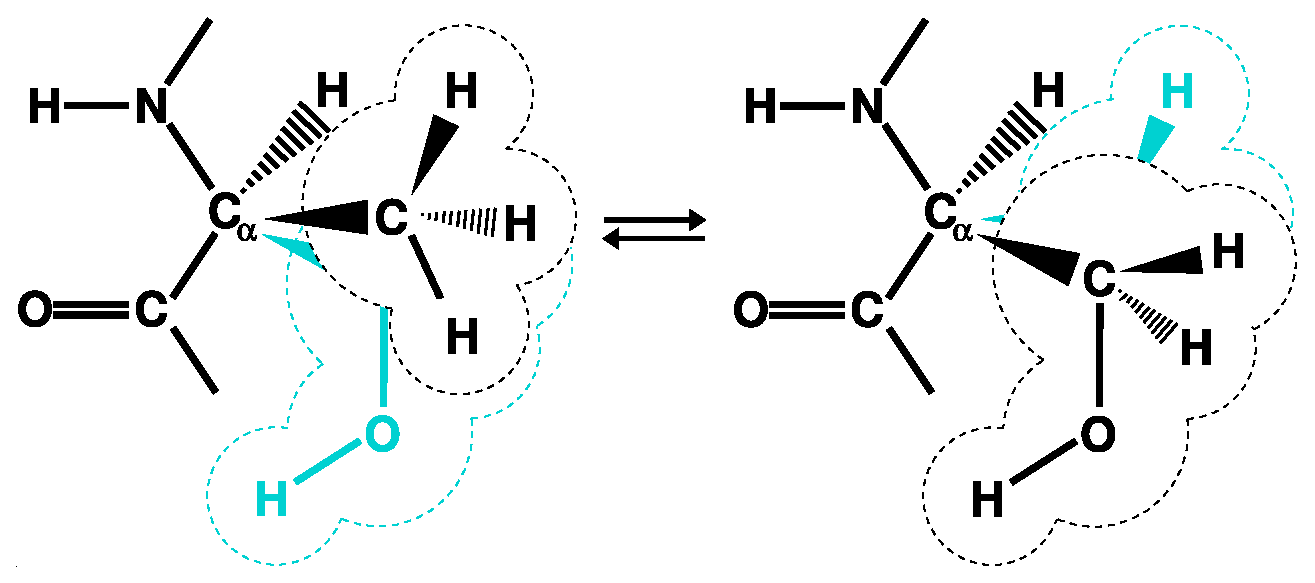
\includegraphics[width=14.5cm]{figures/dual_top}}
  \caption{Dual topology description for an alchemical simulation.
         Case example of the mutation of alanine into glycine.
         The lighter color denotes the non--interacting, alternate
         state.}
  \label{fig:dual_top}
\end{figure}


The energy and forces
are defined as a function of $\lambda$, in such a fashion that 
the interaction of the methyl group of alanine with the rest of 
the protein is effective at the beginning of the simulation,
\ie $\lambda$ = 0, while
the glycine C$_\alpha$ hydrogen does not interact with the rest
of the protein, and {\it vice versa} at the end of the
simulation, \ie $\lambda$ = 1.
For intermediate values of $\lambda$, both the alanine and the glycine
side chains participate in the non--bonded interactions with the rest 
of the protein, scaled on the basis of the current value of $\lambda$.
It should be emphasized that these side chains, however,
do not interact with each other.


It is, therefore, necessary to exclude {\it explicitly} in the setup
those atoms 
that are created from those that will be annihilated in the 
course of the \FEP\ calculation (see ``A tutorial to set up 
alchemical free energy perturbation calculations in \NAMD''
available from the \NAMD\ website).


It is also worth noting that
the free energy calculation does not alter intramolecular
potentials, \ie bond stretch, valence angle deformation, torsions
{\it etc}, during the simulation.
In calculations targetted at the estimation
of free energy differences between two states characterized by
distinct environments --- \eg a ligand bound to a protein in
the first simulation,
and solvated in water, in the second --- as is the 
case for most free energy calculations that make use of a thermodynamic 
cycle, perturbation of intramolecular terms, 
\eg chemical bonds, can be safely
avoided.~\cite{Boresch.99a}



\subsubsection{Implementation of free energy perturbation in \NAMD}


The procedure implemented in \NAMD\ is particularly
adapted for performing free 
energy calculations that split the reaction path into a number of non--physical,
intermediate $\lambda$--states, or ``windows''. Separate simulations 
can be started for each window.
Alternatively, the {\sc Tcl} scripting ability of 
\NAMD\ can be employed advantageously
to perform the complete simulation in a single run.
An example making use of such script is supplied at the end 
of this section.


The following keywords can be used to control free 
energy calculations aimed at alchemical transformations. 

\begin{itemize}

\item
\NAMDCONFWDEF{fep}{ Is alchemical \FEP\ to be performed? }
{{\tt on} or {\tt off}}
{{\tt off}}
{Turns on Hamiltonian scaling and ensemble averaging for alchemical \FEP.}

\item
\NAMDCONF{lambda}{ Coupling parameter value }
{positive decimal between 0.0 and 1.0}
{The coupling parameter value determining the progress of the
perturbation. The non--bonded interactions involving the atoms vanishing
in the course of the MD simulation are scaled by (1-{\tt lambda}), while
those of the growing atoms are scaled by {\tt lambda}.}

\item
\NAMDCONF{lambda2}{Coupling parameter comparison value}
{positive decimal between 0.0 and 1.0}
{The {\tt lambda2} value corresponds to the coupling parameter to be
used for sampling in the next window.  The free energy difference
between {\tt lambda2} and {\tt lambda} is calculated.  Through simulations
at progressive values of {\tt lambda} and {\tt lambda2} the total free
energy difference may be determined.}

\item
\NAMDCONFWDEF{fepEquilSteps}{Number of equilibration steps in the window, 
before data collection}
{positive integer less than {\tt numSteps} or {\tt run}}
{0}
{In each window {\tt fepEquilSteps} steps of equilibration can be
performed before ensemble averaging is initiated. The output also contains
the data gathered during equilibration and is meant for analysis of
convergence properties of the \FEP\ calculation.}

\item
\NAMDCONFWDEF{fepFile}{{\tt pdb} file with perturbation flags}
{filename}
{coordinates}
{{\tt pdb} file to be used for indicating the \FEP\ status for each of
the atoms pertaining to the system. 
If this parameter is not declared specifically, then the
{\tt pdb} file containing the initial coordinates specified by
{\tt coordinates} is utilized for this information.}

\item
\NAMDCONFWDEF{fepCol}{Column in the {\tt fepFile} that carries 
                      the perturbation flag}
{X, Y, Z, O or B}
{B}
{Column of the {\tt pdb} file to use for retrieving the \FEP\ status 
of each atom, \ie a flag that indicates which atom will be perturbed
in the course of the simulation.
A value of {\tt -1} in the specified column indicates the atom will
vanish during the \FEP\ calculation, whereas a value of {\tt 1} 
indicates that the atom will grow.}

\item
\NAMDCONFWDEF{fepOutFreq}{Frequency of \FEP\ energy output in time--steps}
{positive integer}
{5}
{Every {\tt fepOutFreq} number of MD steps, the output file
{\tt fepOutFile} is updated by dumping energies that are
used for ensemble averaging.
This variable could be set to {\tt 1} to include all the 
configurations for ensemble averaging. Yet, it is recommended
to update {\tt fepOutFile}  energies at longer intervals
to avoid large correlation between consecutive configurations.}

\item
\NAMDCONFWDEF{fepOutFile}{\FEP\ energy output filename}
{filename}
{outfilename}
{An output file named {\tt fepOutFile}.fep, generated by \NAMD,
contains the \FEP\ energies, dumped every {\tt fepOutFreq} steps.}

\item
\NAMDCONFWDEF{fepVdWShiftCoeff}{\FEP\ radius-shifting coefficient}
{positive decimal}
{5.}
{This is a radius-shifting coefficient of $\lambda$ that is used 
to construct the modified vdW interactions during alchemical FEP. Providing a positive value for {\tt fepVdWShiftCoeff} ensures that the vdW potential is finite everywhere for small values of $\lambda$, which significantly improves the accuracy and convergence of FEP calculations, and also prevents overlapping particles from making the simulation unstable. During FEP, the inter-atomic distances used in the Lennard-Jones potential are shifted
according to: \\
$r^2 \rightarrow r^2 + {\rm fepVdWShiftCoeff} \times (1. - \lambda)$
}

\item
\NAMDCONFWDEF{fepVdwScaleExp}{\FEP\ Lennerd-Jones parameter scaling exponent}
{decimal}
{0.}
{When constructing the modified vdW interactions during alchemical FEP, the Lennard-Jones parameters are scaled according to:\\
$A \rightarrow A \times \lambda^{2 \times {\rm fepVdwScaleExp}}$ \\
$B \rightarrow B \times \lambda^{\rm fepVdwScaleExp}$
}

%\item
%\NAMDCONFWDEF{fepElecLambdaDelay}{\FEP\ lambda ``delay" for electrostatics}
%{positive decimal}
%{0.}
%{In order to avoid the FEP ``end-point catastrophe", it is often important to make sure that a growing particle does not have an unbounded potential right when it is created (in case that it appears on top of another particle). One way to deal with this for electrostatic interactions, is to allow a bounded scaled vdW potential (using a positive fepVdWShiftCoeff) to first repel all overlapping particles at low values of $\lambda$. As $\lambda$ increases, once the particles are repelled, it is now safe to turn on FEP electrostatics. fepElecLambdaDelay is the value of $\lambda$ at which electrostatic interactins are turned on and start ramping up linearly.}


\end{itemize}


\noindent
{\it Note}: Free energy calculations that rely upon equation~({\ref{master}})
make use of an average temperature, which, in principle, should coincide with
the value of the thermostat. Rather than employing the computed average of $T$,
$\Delta A_{a \rightarrow b}$ is estimated with the target value of the
temperature defined by the user. It is, therefore, necessary to activate
some constant--temperature scheme to carry out \FEP\ calculations. 



\subsubsection{Example of an input file for running \FEP\ alchemical transformations}


The following example illustrates the use of {\sc Tcl} scripting for running
the alchemical \FEP\ feature of \NAMD: 

\begin{verbatim}
fep		on  
fepfile		ion.fep
fepCol		X
fepOutfile	ion.fepout
fepOutFreq	5
fepEquilSteps	5000

set step 0.0
set dstep 0.1

while {$step <= 0.9} {
 lambda $step
 set step [expr $step+$dstep]
 lambda2 $step
 run  10000
}
\end{verbatim}

\noindent
Here, the {\tt pdb} file read by \NAMD\ to extract the information
about perturbed atoms is {\tt biotin.fep}. The pertinent information 
is present in the {\tt X} column. The output file of the free energy
calculation is {\tt biotinr.fepout}, in which energies are written
every {\tt 5} steps.
$\delta \lambda$, the width of the windows, is set to {\tt 0.1}.
{\tt 5000} MD steps are performed in each window to
equilibrate the system. In this particular instance, 
the current value of $\lambda$
is controlled by the statement {\tt set step}. 
The \FEP\ calculation is run until $\lambda$ reaches the
value {\tt 0.9}. In every window, {\tt 10000} MD steps
are performed.


\subsubsection{Description of \FEP\ simulation output }

The {\tt fepOutFile} contains electrostatic and van der Waals energy
data calculated at $\lambda$ and $\lambda2$, written every
{\tt fepOutFreq} steps. The column {\tt dE} is the instantaneous energy
difference for the current configuration. {\tt dE\_avg} and {\tt dG}
are the accumulated energy ensemble average and the corresponding
free energy at the current time step, respectively.
The temperature is specified in the penultimate column. Upon completion
of {\tt fepEquilSteps} steps, the calculation of {\tt dE\_avg} and 
{\tt dG} is restarted. The accumulated net free energy change is output
at each $\lambda$--value and at the end of the simulation. The cumulative
average energy {\tt dE\_avg} value may be summed using, for instance, the 
trapezoidal rule, or a Gaussian quadrature, to obtain an approximate 
TI estimate for the free energy change during the run.





\subsection{Locally Enhanced Sampling}
\label{section:les}

Locally enhanced sampling (LES)~\cite{ROIT91,SIMM98,SIMM00} increases
sampling and transition rates for a portion of a molecule by the use of
multiple non-interacting copies of the enhanced atoms.  These enhanced
atoms experience an interaction (electrostatics, van der Waals, and
covalent) potential that is divided by the number of copies present.
In this way the enhanced atoms can occupy the same space, while the
multiple instances and reduces barriers increase transition rates.

\subsubsection{Structure Generation}

To use LES, the structure and coordinate input files must be modified to
contain multiple copies of the enhanced atoms.  \PSFGEN\ provides the
{\tt multiply} command for this purpose.  \NAMD\ supports a maximum of 15
copies, which should be sufficient.  

Begin by generating the complete molecular structure and guessing
coordinates as described in Sec.~\ref{section:psfgen}.  As the last
operation in your script, prior to writing the psf and pdb files, add
the {\tt multiply} command, specifying the number of copies desired and
listing segments, residues, or atoms to be multiplied.  For example,
\verb#multiply 4 BPTI:56 BPTI:57# will create four copies of the last
two residues of segment BPTI.  You must include all atoms to be
enhanced in a single {\tt multiply} command in order for the bonded
terms in the psf file to be duplicated correctly.  Calling {\tt multiply}
on connected sets of atoms multiple times will produce unpredictable
results, as may running other commands after {\tt multiply}.

The enhanced atoms are duplicated exactly in the structure---they have
the same segment, residue, and atom names.  They are distinguished only
by the value of the B (beta) column in the pdb file, which is 0 for
normal atoms and varies from 1 to the number of copies created for
enhanced atoms.  The enhanced atoms may be easily observed in VMD with
the atom selection \verb#beta != 0#.

\subsubsection{Simulation}

In practice, LES is a simple method used to increase sampling;
no special output is generated.
The following parameters are used to enable LES:

\begin{itemize}

\item
\NAMDCONFWDEF{les}{is locally enhanced sampling active?}{{\tt on} or {\tt
off}}{{\tt off}}
{Specifies whether or not LES is active.}

\NAMDCONF{lesFactor}{number of LES images to use}
{positive integer equal to the number of images present}
{This should be equal to the factor used in {\tt multiply}
 when creating the structure.  The interaction potentials for images is
 divided by {\tt lesFactor}.  
}

\item
\NAMDCONFWDEF{lesReduceTemp}{reduce enhanced atom temperature?}{{\tt on} or {\tt
off}}{{\tt off}}
{Enhanced atoms experience interaction potentials divided by {\tt lesFactor}.
This allows them to enter regions that would not normally be thermally
accessible.  If this is not desired, then the temperature of these atoms
may be reduced to correspond with the reduced potential.  This option
affects velocity initialization, reinititialization, reassignment, and
the target temperature for langevin dynamics.  Langevin dynamics is
recommended with this option, since in a constant energy simulation energy
will flow into the enhanced degrees of freedom until they reach thermal
equilibrium with the rest of the system.  The reduced temperature atoms
will have reduced velocities as well, unless {\tt lesReduceMass} is also
enabled.}

\item
\NAMDCONFWDEF{lesReduceMass}{reduce enhanced atom mass?}{{\tt on} or {\tt off}}{{\tt off}}
{Used with {\tt lesReduceTemp} to restore velocity distribution to
enhanced atoms.  If used alone, enhanced atoms would move faster than
normal atoms, and hence a smaller timestep would be required.}

\item
\item
\NAMDCONFWDEF{lesFile}{PDB file containing LES flags}{UNIX filename} {{\tt coordinates}}
{PDB file to specify the LES image number of each atom.
If this parameter is not specified, then 
the PDB file containing initial coordinates specified by 
{\tt coordinates} is used.}

\item
\NAMDCONFWDEF{lesCol}{column of PDB file containing LES flags}{{\tt X}, {\tt Y}, {\tt Z}, {\tt O}, or {\tt B}}{{\tt B}}
{Column of the PDB file to specify the LES image number of each atom.
This parameter may specify any of the floating point fields of the PDB file, 
either X, Y, Z, occupancy, or beta-coupling (temperature-coupling).  
A value of 0 in this column indicates that the atom is not enhanced.
Any other value should be a positive integer less than {\tt lesFactor}.}

\end{itemize}


\subsection{Pair Interaction Calculations}
\label{section:pairinteraction}
\NAMD\ supportes the calculation of interaction energy calculations between 
two groups of atoms.  When enabled, pair interaction information will be
calculated and printed in the standard output file on its own line at the
same frequency as energy output.  The format of the line is
{\tt PAIR INTERACTION: STEP: {\it step} VDW\_FORCE: {\it fx fy fz} 
ELECT\_FORCE: {\it fx fy fz}}.
The displayed force is the force on atoms in group 1 and is units of 
kcal/mol/\AA. 

For trajectory analysis the 
recommended way to use this set of options is to use the NAMD Tcl scripting 
interface as described in Sec.~\ref{section:tclscripting} to run for
0 steps, so that NAMD prints the energy without performing any dynamics.

\begin{itemize}

\item
\NAMDCONFWDEF{pairInteraction}{is pair interaction calculation active?}
{{\tt on} or {\tt off}}{{\tt off}}
{Specifies whether pair interaction calculation is active.}

\item
\NAMDCONFWDEF{pairInteractionFile}{PDB file containing pair interaction flags}
{UNIX filename}{{\tt coordinates}}
{PDB file to specify atoms to use for pair interaction calculations.  If 
this parameter is not specified, then the PDB file containing initial 
coordinates specified by {\tt coordinates} is used.}

\item
\NAMDCONFWDEF{pairInteractionCol}{column of PDB file containing pair 
interaction flags}{{\tt X}, {\tt Y}, {\tt Z}, {\tt O}, or {\tt B}}{{\tt B}}
{
Column of the PDB file to specify which atoms to use for pair interaction
calculations.  This parameter may specify any of the floating point
fields of the PDB file, either X, Y, Z, occupancy, or beta-coupling
(temperature-coupling).  
}

\item
\NAMDCONFWDEF{pairInteractionSelf}{compute within-group interactions instead of
bewteen groups}{{\tt on} or {\tt off}}{{\tt off}}
{
When active, NAMD will compute bonded and nonbonded interactions only for atoms 
within group 1.  
}
 
\item
\NAMDCONF{pairInteractionGroup1}{Flag to indicate atoms in
group 1?}{integer}{}

\item
\NAMDCONF{pairInteractionGroup2}{Flag to indicate atoms in
group 2?}{integer}{}
{
These options are used to indicate which atoms belong to each interaction 
group.  Atoms with a value in the column specified by {\tt pairInteractionCol} 
equal to {\tt pairInteractionGroup1} will be assigned to group 1; likewise
for group 2.
}

\subsection{Pressure Profile Calculations}
\NAMD\ supports the calculation of lateral pressure profiles as a function of
the z-coordinate in the system.  The algorithm is based on that of 
Lindahl and Edholm (JCP 2000), with modifications to enable Ewald sums based on
Sonne et al (JCP 122, 2005). 

The simulation space is partitioned into slabs, and half the virial
due to the interaction between two particles is assigned to each
of the slabs containing the particles.  This amounts to employing
the Harasima contour, rather than the Irving-Kirkwood contour, as
was done in \NAMD\ 2.5.  The diagonal components of the pressure
tensor for each slab, averaged over all timesteps since the previous
output, are recorded in the \NAMD\ output file.  The
units of pressure are the same as in the regular \NAMD\ pressure
output; i.e., bar.

The total virial contains contributions from up to four components: 
kinetic energy, bonded interactions, nonbonded interactions, and an Ewald
sum.  All but the Ewald sums are computed online during a normal simulation
run (this is a change from \NAMD\ 2.5, when nonbonded contributions to the
Ewald sum were always computed offline).  If the simulations are performed
using PME, the Ewald contribution should be estimated using a separate,
offline calculation based on the saved trajectory files.  The nonbonded
contribution using a cutoff different from the one used in the simulation
may also be computed offline in the same fashion as for Ewald, if desired.

Pressure profile calculations may be performed in either constant volume 
or constant pressure conditions.  If constant pressure is enabled, the
slabs thickness will be rescaled along with the unit cell; the dcdUnitCell
option will also be switched on so that unit cell information is stored in
the trajectory file.

\NAMD\ 2.6 now reports the lateral pressure partitioned by interaction type.
Three groups are reported: kinetic + rigid bond restraints (referred to as 
``internal", bonded, and nonbonded.  If Ewald pressure profile calculations
are active, the Ewald contribution is reported in the nonbonded section, and
no other contributions are reported.

\NAMD\ 2.6 also permits the pressure profile to be partitioned by atom type.
Up to 15 atom groups may be assigned, and individual contribution of each
group (for the ``internal" pressures) and the pairwise contributions of
interactions within and between groups (for the nonbonded and bonded pressures)
are reported in the output file.

\item
\NAMDCONFWDEF{pressureProfile}{compute pressure profile}{{\tt on} or {\tt off}}{{\tt off}}
{
When active, NAMD will compute kinetic, bonded and nonbonded (but not 
reciprocal space) contributions to the 
pressure profile.  Results will be recorded in the \NAMD\ output file
in lines with the format
{\tt PRESSUREPROFILE: ts Axx Ayy Azz Bxx Byy Bzz ... }, where {\tt ts} is the
timestep, followed by the three diagonal components of the pressure tensor 
in the first
slab (the slab with lowest {\it z}), then the next lowest slab, and so forth.
The output will reflect the pressure profile averaged over all the steps since
the last output.  

\NAMD\ also reports kinetic, bonded and nonbonded contributions separately,
using the same format as the total pressure, but on lines beginning with
{\tt PPROFILEINTERNAL}, {\tt PPROFILEBONDED}, and {\tt PPROFILENONBONDED}.
}
\item
\NAMDCONFWDEF{pressureProfileSlabs}{Number of slabs in the spatial partition}{Positive integer}{10}{
\NAMD\ divides the entire periodic cell into horizontal slabs of equal 
thickness; {\tt pressureProfileSlabs} specifies the number of such slabs.
}

\item
\NAMDCONFWDEF{pressureProfileFreq}{How often to output pressure profile
data}{Positive integer}{1}{
Specifies the number of timesteps between output of pressure profile data.
}

\item
\NAMDCONFWDEF{pressureProfileEwald}{Enable pressure profile Ewald sums}{{\tt on} or {\tt off}}{{\tt off}}{
When enabled, only the Ewald contribution to the pressure profile will be
computed.  For trajectory analysis the 
recommended way to use this option is to use the \NAMD\ Tcl scripting 
interface as described in Sec.~\ref{section:tclscripting} to run for
0 steps, so that NAMD prints the pressure profile without performing any 
dynamics.

The Ewald sum method is as described in Sonne et al. (JCP 122, 2005).  The
number of $k$ vectors to use along each periodic cell dimension is specified
by the {\tt pressureProfileEwald}$n$ parameters described below.
}
\item
\NAMDCONFWDEF{pressureProfileEwaldX}{Ewald grid size along X}
{Positive integer}{10}{}
\item
\NAMDCONFWDEF{pressureProfileEwaldY}{Ewald grid size along Y}
{Positive integer}{10}{}
\item
\NAMDCONFWDEF{pressureProfileEwaldZ}{Ewald grid size along Z}
{Positive integer}{10}{}

\item
\NAMDCONFWDEF{pressureProfileAtomTypes}{Number of atom type partitions}{Positive integer}{1}{
If {\tt pressureProfileAtomTypes} is greater than 1, \NAMD\ will calculate
the separate contributions of each type of atom to the internal, bonded, 
nonbonded, and total pressure.  In the case of the internal contribution,
there will be $n$ pressure profile data sets reported on each 
{\tt PPROFILEINTERNAL} line, where $n$ is the number of atom types. All the 
partial pressures for atom type 1 will be followed by those for atom type 2,
and so forth.  The other three pressure profile reports will contain 
$n(n+1)/2$ data sets.  For example, if there are $n=3$ atom types, the
six data sets arising from the three inter-partition and the three 
intra-partition interactions will be reported in the following order:
1--1, 1--2, 1--3, 2--2, 2--3, 3--3.  The total pressure profile, reported
on the {\tt PRESSUREPROFILE} line, will contain the internal contributions 
in the data sets corresponding to 1--1, 2--2, etc.  
}

\item
\NAMDCONFWDEF{pressureProfileAtomTypesFile}{Atom type partition assignments}
{PDB file}{coordinate file}{
If {\tt pressureProfileAtomTypes} is greater than 1, NAMD will assign
atoms to types based on the corresponding value in {\tt pressureProfileAtomTypesCol}.  The type for each atom must be strictly less than 
{\tt pressureProfileAtomTypes}!}

\item
\NAMDCONFWDEF{pressureProfileAtomTypesCol}{{\tt pressureProfileAtomTypesFile}
PDB column}{PDB file}{B}{}

\end{itemize}

Here is an example snippet from a \NAMD\ input that can be used to compute
the Ewald component of the pressure profile.  It assumes that the 
coordinates were saved in the dcd file {\tt pp03.dcd}) every 500 timesteps.  
\begin{verbatim}

Pme             on
PmeGridSizeX    64
PmeGridSizeY    64
PmeGridSizeZ    64

exclude         scaled1-4
1-4scaling      1.0  

switching on
switchdist      9
cutoff          10
pairlistdist    11

pressureProfile        on
pressureProfileSlabs   30
pressureProfileFreq    100
pressureProfileAtomTypes 6
pressureProfileAtomTypesFile atomtypes.pdb
pressureProfileEwald  on
pressureProfileEwaldX  16
pressureProfileEwaldY  16
pressureProfileEwaldZ  16

set ts 0
firstTimestep $ts

coorfile open dcd pp03.dcd
while { [coorfile read] != -1 } {
  incr ts 500
  firstTimestep $ts
  run 0
}
coorfile close
\end{verbatim}


\subsection{Replica Exchange Simulations}

\index{replica exchange}
The {\tt lib/replica/}
directory contains Tcl scripts that implement replica exchange
for NAMD, using a Tcl server and socket connections to drive a
separate NAMD process for every replica used in the simulation.
Replica exchanges and energies are recorded in the potenergy.dat,
realtemp.dat, and targtemp.dat files written in the output directory.
These can be viewed with, e.g., ``{\tt xmgrace -nxy ....potenergy.dat}''
There is also a script to load the output into VMD and color each
frame according to target temperature.  An example simulation folds
a 66-atom model of a deca-alanine helix in about 10\,ns.

This implementation is designed to be modified by the user to implement
exchanges of parameters other than temperature or via other temperature
exchange methods.  The scripts should provide a good starting point for
any simulation method requiring a number of loosely interacting systems.

{\tt replica\_exchange.tcl}
is the master Tcl script for replica exchange simulations, it is run in
{\tt tclsh} {\em outside of NAMD} and takes a replica exchange config
file as an argument:
\begin{verbatim}
          tclsh ../replica_exchange.tcl fold_alanin.conf
          tclsh ../replica_exchange.tcl restart_1.conf
\end{verbatim}
{\tt replica\_exchange.tcl} uses code in
{\tt namd\_replica\_server.tcl}, a general script for driving NAMD slaves, and
{\tt spawn\_namd.tcl}, a variety of methods for launching NAMD slaves.

{\tt show\_replicas.vmd} is a script for loading replicas into VMD;
first source the replica exchange conf file and then this script, then
repeat for each restart conf file or for example just do
``{\tt vmd -e load\_all.vmd}''.
This script will likely destroy anything else you are doing in VMD at the
time, so it is best to start with a fresh VMD.
{\tt clone\_reps.vmd} provides the {\tt clone\_reps} commmand to copy graphical
representation from the top molecule to all other molecules.

A replica exchange config file should define the following Tcl variables:
\begin{itemize}
\item {\tt num\_replicas}, the number of replica simulations to use,
\item {\tt min\_temp}, the lowest replica target temperature,
\item {\tt max\_temp}, the highest replica target temperature,
\item {\tt steps\_per\_run}, the number of steps between exchange attempts,
\item {\tt num\_runs}, the number of runs before stopping
(should be divisible by {\tt runs\_per\_frame} $\times$ {\tt frames\_per\_restart}).
\item {\tt runs\_per\_frame}, the number of runs between trajectory outputs,
\item {\tt frames\_per\_restart}, the number of frames between restart outputs,

\item {\tt namd\_config\_file}, the NAMD config file containing all parameters,
needed for the simulation except {\tt seed}, {\tt langevin}, 
{\tt langevinDamping}, {\tt langevinTemp}, {\tt outputEnergies},
{\tt outputname}, {\tt dcdFreq},
{\tt temperature}, {\tt bincoordinates}, {\tt binvelocities},
or {\tt extendedSystem}, which are provided by {\tt replica\_exchange.tcl},

\item {\tt output\_root}, the directory/fileroot for output files,

\item {\tt psf\_file}, the psf file for {\tt show\_replicas.vmd}, 
\item {\tt initial\_pdb\_file}, the initial coordinate pdb file for {\tt show\_replicas.vmd},
\item {\tt fit\_pdb\_file}, the coodinates that frames are fit to by {\tt show\_replicas.vmd} (e.g., a folded structure),
\item {\tt server\_port}, the port to connect to the replica server on, and
\item {\tt spawn\_namd\_command}, a command from {\tt spawn\_namd.tcl} and arguments to launch NAMD jobs.
\end{itemize}

The {\tt lib/replica/example/} directory contains
all files needed to fold a 66-atom model of a deca-alanine helix:
\begin{itemize}
\item {\tt alanin\_base.namd}, basic config options for NAMD,
\item {\tt alanin.params}, parameters,
\item {\tt alanin.psf}, structure,
\item {\tt unfolded.pdb}, initial coordinates,
\item {\tt alanin.pdb}, folded structure for fitting in {\tt show\_replicas.vmd},
\item {\tt fold\_alanin.conf}, config file for {\tt replica\_exchange.tcl} script,
\item {\tt restart\_1.conf}, config file to continue alanin folding another 10\,ns, and
\item {\tt load\_all.vmd}, load all output into VMD and color by target temperature.
\end{itemize}

The {\tt fold\_alanin.conf} config file contains the following settings:
\begin{verbatim}
set num_replicas 8
set min_temp 300
set max_temp 600
set steps_per_run 1000
set num_runs 10000
set runs_per_frame 10
set frames_per_restart 10
set namd_config_file "alanin_base.namd"
set output_root "output/fold_alanin" ; # directory must exist
set psf_file "alanin.psf"
set initial_pdb_file "unfolded.pdb"
set fit_pdb_file "alanin.pdb"
set namd_bin_dir /Projects/namd2/bin/current/Linux64
set server_port 3177
set spawn_namd_command \
  [list spawn_namd_ssh "cd [pwd]; [file join $namd_bin_dir namd2] +netpoll" \
  [list beirut belfast] ]
\end{verbatim}

